\documentclass[fontsize=11pt, twoside=false, numbers=autoenddot]{scrbook}
\usepackage{automaten_tafelanschriebe}

\pagestyle{plain}
% \pagestyle{scrheadings}
% % \chead{\headmark}
% \chead{\partmark}
% \renewcommand{\sectionmark}[1]{\markright{\textsl{#1}}}
% \renewcommand{\chaptermark}[1]{\markright{\textsl{#1}}{}}
% \renewcommand{\partmark}[1]{\markright{\textsl{#1}}}
\parindent0pt
\parskip\smallskipamount

\title{Tafelmitschriften zur Vorlesung \glqq Automatentheorie und ihre Anwendungen\grqq\\ im Wintersemester 2019/20}
\author{%
  Prof.\ Dr.\ Thomas Schneider\\[1pt]
  AG Theorie der Künstlichen Intelligenz \\[1pt]
  Fachbereich 3 \\
  
\includegraphics[width=.4\linewidth]{logo_ub.jpg} \\[\baselineskip]~%
}
\date{Stand: \today}
%\publishers{{\large Dieses Dokument ist noch unvollständig und wird regelmäßig aktualisiert.}}

\begin{document}

\maketitle
\tableofcontents

% ===================================================================
% ===================================================================
% ===================================================================
\part[Endliche Automaten auf endlichen Wörtern]{Endliche Automaten \\ auf endlichen Wörtern}

% ===================================================================
\section*{T1.1~ Beispiel für Papierkorbzustand}

Der NEA $\Amc_1$ von Folie 1.10
%
\vspace*{-.7\baselineskip}
\begin{center}
  \begin{tikzpicture}[%
    node distance=20mm,>=Latex,
    initial text="", initial where=below left,
    every state/.style={draw=black,thin,fill=black!5,inner sep=1mm,minimum size=6mm},
    accepting/.style={double distance=1.5pt, double=white},
    every edge/.style={draw=black,thin}
  ]
    \node[state,initial]                          (q0) {$q_0$};
    \node[state,accepting]                        (q1) [right of=q0] {$q_1$};
    \node[state,draw=white,fill=white,text=white] (m)  [right of=q1] {$m$};
    \node[above left=-2mm and 6mm of q0] {$\Amc_1$};
    
    \path[->]
      (q0) edge                    node [above]                {$b$} (q1)
      (q0) edge [loop above]       node [right=1mm]            {$a$} ()
      (q1) edge [loop above]       node [right=1mm]            {$b$} ()
      (m)  edge [white,loop above] node [right=1mm,text=white] {$a,b$} ()
      ;
  \end{tikzpicture}
\end{center}
%
ist nur deshalb kein DEA, weil Zustand $q_1$ keine ausgehende $b$-Kante besitzt.
Durch Hinzufügen eines neuen Zustands $m$ (für "`Mülleimer"' oder "`Papierkorb"')
wird $\Amc_1$ zu einem DEA $\Amc_1'$, ohne dass das Akzeptanzverhalten sich ändert:
%
\vspace*{-.2\baselineskip}
\begin{center}
  \begin{tikzpicture}[%
    node distance=20mm,>=Latex,
    initial text="", initial where=below left,
    every state/.style={draw=black,thin,fill=black!5,inner sep=1mm,minimum size=6mm},
    accepting/.style={double distance=1.5pt, double=white},
    every edge/.style={draw=black,thin}
  ]
    \node[state,initial]   (q0) {$q_0$};
    \node[state,accepting] (q1) [right of=q0] {$q_1$};
    \node[state]           (m)  [right of=q1] {$m$};
    \node[above left=-2mm and 6mm of q0] {$\Amc_1'$};
    
    \path[->]
      (q0) edge              node [above] {$b$} (q1)
      (q1) edge              node [above] {$a$} (m)
      (q0) edge [loop above] node [right=1mm] {$a$} ()
      (q1) edge [loop above] node [right=1mm] {$b$} ()
      (m)  edge [loop above] node [right=1mm] {$a,b$} ()
      ;
  \end{tikzpicture}
\end{center}
%
Diese Konstruktion macht aber beispielsweise aus dem NEA $\Amc_3$ von Folie 1.10
\emph{keinen} DEA, denn dabei behält $q_0$ seine \emph{zwei} $a$-Nachfolger.

% ===================================================================
\section*{T1.2~ Beispiel für die Potenzmengenkonstruktion}

Wir betrachten den NEA $\Amc_3$ von Folie 1.10:
%
\vspace*{-.2\baselineskip}
\begin{center}
  \begin{tikzpicture}[%
    node distance=20mm,>=Latex,
    initial text="", initial where=below left,
    every state/.style={draw=black,thin,fill=black!5,inner sep=1mm,minimum size=6mm},
    accepting/.style={double distance=1.5pt, double=white},
    every edge/.style={draw=black,thin}
  ]
    \node[state,initial]   (q0) {$q_0$};
    \node[state]           (q1) [right of=q0] {$q_1$};
    \node[state,accepting] (q2) [right of=q1] {$q_2$};
    \node[above left=-2mm and 6mm of q0] {$\Amc_3$};
    
    \path[->]
      (q0) edge              node [above] {$a$} (q1)
      (q1) edge              node [above] {$b$} (q2)
      (q0) edge [loop above] node [right=1mm] {$a,b$} ()
      ;
  \end{tikzpicture}
\end{center}
%
Wenn man die Potenzmengenkonstruktion (Folie 1.13) ausführt,
und dabei die unerreichbaren Zustände ignoriert,
dann erhält man folgenden DEA $\Amc_3^d$.
%
\vspace*{-.2\baselineskip}
\begin{center}
  \begin{tikzpicture}[%
    node distance=20mm,>=Latex,
    initial text="", initial where=below left,
    every state/.style={ellipse,draw=black,thin,fill=black!5,inner sep=1mm,minimum size=6mm},
    accepting/.style={double distance=1.5pt, double=white},
    every edge/.style={draw=black,thin}
  ]
    \node[state,initial]   (q0)                                     {$\{q_0\}$};
    \node[state]           (q0q1) [right=30mm of q0]                {$\{q_0,q_1\}$};
    \node[state,accepting] (q0q2) [below right=5mm and 10mm of q0] {$\{q_0,q_2\}$};
    \node[above left=-2mm and 6mm of q0] {$\Amc_3^d$};
    
    \path[->]
      (q0)   edge [loop above]    node [right=1mm]        {$b$} ()
      (q0)   edge                 node [above]            {$a$} (q0q1)
      (q0q1) edge [loop above]    node [right=1mm]        {$a$} ()
      (q0q1) edge [bend right=10] node [pos=.3,left=2mm]  {$b$} (q0q2)
      (q0q2) edge [bend right=10] node [pos=.3,right=2mm] {$a$} (q0q1)
      (q0q2) edge                 node [pos=.7,right=2mm] {$b$} (q0)
      ;
  \end{tikzpicture}
\end{center}

\enlargethispage*{20mm}
\vspace*{-\baselineskip}
% ===================================================================
\section*{T1.3~ Beispiel-NEA für Stichwortsuche}

Seien $w_1 = \texttt{web}$ und $w_2 = \texttt{ebay}$,
und sei $\Sigma$ die Menge aller ASCII-Zeichen.
Folgender NEA $\Amc$ akzeptiert genau die Dokumente (Zeichenketten),
die $w_1$ oder $w_2$ als Teilwort enthalten.
Dies gilt aber nur, wenn die leicht geänderte Akzeptanzbedingung von Folie~1.17
zugrunde gelegt wird:
$\Amc$ akzeptiert, sobald ein akzeptierender Zustand erreicht wird,
auch wenn das Eingabewort zu diesem Zeitpunkt noch nicht zu Ende gelesen wurde.
%
\vspace*{-.2\baselineskip}
\begin{center}
  \begin{tikzpicture}[%
    node distance=20mm,>=Latex,
    initial text="", initial where=below left,
    every state/.style={draw=black,thin,fill=black!5,inner sep=1mm,minimum size=6mm},
    accepting/.style={double distance=1.5pt, double=white},
    every edge/.style={draw=black,thin}
  ]
    \node[state,initial]                       (0) {0};
    \node[state,above right=1mm and 10mm of 0] (1) {1};
    \node[state,right of=1]                    (2) {2};
    \node[state,accepting,right of=2]          (3) {3};
    \node[state,below right=1mm and 10mm of 0] (4) {4};
    \node[state,right of=4]                    (5) {5};
    \node[state,right of=5]                    (6) {6};
    \node[state,accepting,right of=6]          (7) {7};
    \node[above left=-2mm and 6mm of 0] {$\Amc$};
    
    \path[->]
      (0) edge [loop below] node [below]            {$\Sigma$} ()
      (0) edge              node [pos=.9,left=2mm]  {\texttt{w}} (1)
      (1) edge              node [above]            {\texttt{e}} (2)
      (2) edge              node [above]            {\texttt{b}} (3)
      (0) edge              node [pos=.1,right=2mm] {\texttt{e}} (4)
      (4) edge              node [above]            {\texttt{b}} (5)
      (5) edge              node [above]            {\texttt{a}} (6)
      (6) edge              node [above]            {\texttt{y}} (7)
      ;
  \end{tikzpicture}
\end{center}
%
Die Beschriftung $\Sigma$ der Schleife am Zustand 0
steht für die Folge aller Symbole aus $\Sigma$.

\pagebreak
% ===================================================================
\section*{T1.4~ Beispiel-DEA für Stichwortsuche}

Um die Determinisierung in diesem speziellen Fall zu demonstrieren,
wählen wir ein einfacheres Beispiel der Stichwortsuche:
wir beschränken uns auf das Alphabet $\Sigma=a,b,c$
und die Stichwörter $w_1=ab$, $w_2=bc$ und $w_3=ca$.
Analog zu T1.3 erhält man folgenden NEA \Amc.
%
\begin{center}
  \begin{tikzpicture}[%
    node distance=30mm,>=Latex,
    initial text="", initial where=below left,
    every state/.style={draw=black,thin,fill=black!5,inner sep=1mm,minimum size=6mm},
    accepting/.style={double distance=1.5pt, double=white},
    every edge/.style={draw=black,thin}
  ]
    \node[state,initial]              (0) {0};
    \node[state,right of=0]           (3) {3};
    \node[state,accepting,right of=3] (4) {4};
    \node[state,above=4mm of 3]       (1) {1};
    \node[state,accepting,right of=1] (2) {2};
    \node[state,below=4mm of 3]       (5) {5};
    \node[state,accepting,right of=5] (6) {6};
    \node[above left=-2mm and 6mm of 0] {$\Amc$};
    
    \path[->]
      (0) edge [loop below] node [below]            {$a,b,c$} ()
      (0) edge              node [pos=.75,left=2mm]  {$a$}     (1)
      (0) edge              node [pos=.6,above]     {$b$}     (3)
      (0) edge              node [pos=.45,right=2mm] {$c$}     (5)
      (1) edge              node [above]            {$b$}     (2)
      (3) edge              node [above]            {$c$}     (4)
      (5) edge              node [above]            {$a$}     (6)
      ;
  \end{tikzpicture}
\end{center}
%
Wendet man die Potenzmengenkonstruktion an
und beschränkt sich dabei wieder auf die erreichbaren Zustände,
dann erhält man folgenden DEA $\Amc^d$.
%
\vspace*{-2\baselineskip}
\begin{center}
  \begin{tikzpicture}[%
    node distance=30mm,>=Latex,
    initial text="", initial where=below left,
    every state/.style={draw=black,thin,fill=black!5,inner sep=.5mm,minimum size=8mm},
    accepting/.style={double distance=1.5pt, double=white},
    every edge/.style={draw=black,thin}
  ]
    \node[state,initial]               (0)   {0};
    \node[state,right of=0]            (03)  {03};
    \node[state,accepting,right of=03] (045) {045};
    \node[state,above=9mm of 3]        (01)  {01};
    \node[state,accepting,right of=01] (023) {023};
    \node[state,below=9mm of 3]        (05)  {05};
    \node[state,accepting,right of=05] (016) {016};
    \node[above left=-2mm and 6mm of 0] {$\Amc^d$};
    
    \path[->]
      (0)   edge                 node [pos=.7,left=2mm]  {$a$} (01)
      (0)   edge                 node [above]            {$b$} (03)
      (0)   edge                 node [pos=.3,right=2mm] {$c$} (05)
      (01)  edge [loop above]    node [above]            {$a$} ()
%      (03)  edge [loop above]    node [above]            {$b$} ()
      (03) edge [out=75,in=45,loop] node [right=0mm]     {$b$} ()
      (05)  edge [loop below]    node [below]            {$c$} ()
      (01)  edge [bend right=45] node [pos=.3,left]      {$c$} (05)
      (03)  edge                 node [left]             {$a$} (01)
      (05)  edge                 node [left]             {$b$} (03)
      (01)  edge [bend left=10]  node [above]            {$b$} (023)
      (03)  edge [bend left=10]  node [above]            {$c$} (045)
      (05)  edge [bend left=10]  node [above]            {$a$} (016)
      (023) edge [bend left=10]  node [below]            {$a$} (01)
      (045) edge [bend left=10]  node [below]            {$b$} (03)
      (016) edge [bend left=10]  node [below]            {$c$} (05)
      (023) edge                 node [right]            {$c$} (045)
      (045) edge                 node [right]            {$a$} (016)
      (016) edge [bend right=45] node [pos=.3,right]     {$b$} (023)
      (023) edge                 node [pos=.4,right=3mm] {$b$} (03)
      (045) edge                 node [pos=.4,right=3mm] {$c$} (05)
      (016) edge [out=10,in=40,looseness=2]  node [pos=.2,right]     {$a$} (01)
      ;
  \end{tikzpicture}
\end{center}
%
Dabei sind die Zustandsnamen wie 01, 023 usw.\
Kurzschreibweisen für die Mengen $\{0,1\}$, $\{0,2,3\}$ usw.

Die Anzahl der Zustände von $\Amc^d$ ist genauso groß wie die von $\Amc$,
und man kann zeigen, dass dies für jeden NEA $\Amc$ der Fall ist,
den man für die Stichwortsuche gemäß der Beispiele in T1.3 und T1.4 konstruiert.
Der DEA hat also immer nur $|w_1| + \dots + |w_n|$ Zustände,
wenn $w_1,\dots,w_n$ die Stichwörter sind.

%\goodbreak
\pagebreak
% ===================================================================
\section*{T1.5~ Beispiel für die Anwendung des Pumping-Lemmas}

Wir betrachten die Sprache $L = \{a^nb^n \mid n \geq 0\}$.

\textsf{\textbf{Vorbetrachtung für Lesende, die mehr Hintergrundinfo benötigen.}}~
Intuitiv kann diese Sprache nicht NEA-erkennbar sein,
weil NEAs nicht unbeschränkt zählen können --
insbesondere kann ein NEA nicht die Anzahl der gelesenen $a$'s
speichern, um diese mit der Anzahl der $b$'s zu vergleichen.
Dies bleibt aber ein intuitives Argument, denn es basiert auf der
(schwer zu beweisenden) Annahme, dass die skizzierte Vorgehensweise
die einzig mögliche ist.

Um unanfechtbar zu beweisen, dass $L$ nicht NEA-erkennbar ist, verwenden wir
die Kontraposition des Pumping-Lemmas. Wir müssen also zeigen:
%
\begin{enumerate}
  \item
    Für alle $p \geq 0$
  \item
    gibt es ein Wort $w \in L$ mit $|w| \geq p$, so dass gilt:
  \item
    für alle Zerlegungen $w=xyz$ mit $y \neq \varepsilon$ und $|xy| \leq p$
  \item
    gibt es ein $i \geq 0$ mit $xy^iz \notin L$.
\end{enumerate}
%
In den Schritten 1 und 3 ("`für alle"') müssen wir
für eine \emph{beliebige} Zahl $p$ bzw.\ Zerlegung $xyz$ argumentieren;
in Schritten 2 und 4 ("`es gibt"') genügt es, ein Wort $w$ bzw.\ ein $i \geq 0$ zu wählen
(in Abhängigkeit von $p$ bzw.\ $xyz$).

\textsf{\textbf{Eigentlicher Beweis.}}~
Sei $p \geq 0$ beliebig. Wir wählen $w=a^pb^p$, für das offensichtlich $w \in L$ mit $|w| \geq p$ gilt.
Sei nun $w=xyz$ eine beliebige Zerlegung mit $y \neq \varepsilon$ und $|xy| \leq p$.
Wegen $|xy| \leq p$ kann $y$ nur aus $a$'s bestehen.
Wegen $y \neq \varepsilon$ muss $y$ mindestens ein $a$ enthalten.
Wenn wir also nun $i=0$ wählen, dann hat das Wort $xy^0z = xz$ mindestens ein $a$ weniger als $w=xyz$,
aber es hat dieselbe Anzahl $b$'s wie $w$. Deshalb kann $xy^0z$ nicht mehr von der Form $a^nb^n$ sein;
also ist $xy^0z \notin L$.

% ===================================================================
\section*{T1.6~ Beispiel für die Anwendung des Satzes von Myhill-Nerode}

Wir betrachten wieder die Sprache $L = \{a^nb^n \mid n \geq 0\}$.
Es ist leicht zu sehen, dass für zwei beliebige Zahlen $k_1,k_2$
mit $k_1 \neq k_2$ gilt: $a^{k_1} \not\sim_L a^{k_2}$.
Dies ist so, weil beispielsweise für $w=b^{k_1}$ zwar das Wort $a^{k_1}w$
in $L$ liegt, aber das Wort $a^{k_2}w$ nicht.
Deshalb bilden alle $a^k$, $k \geq 0$, paarweise verschiedene Äquivalenzklassen,
und somit ist der Index von $\sim_L$ unendlich.
Mit dem Satz von Myhill-Nerode folgt, dass $L$ nicht NEA-erkennbar ist.

\pagebreak
% ===================================================================
\section*{T1.7~ Beispiel einer Polynomialzeitreduktion}

Wir betrachten die folgenden Mengen.
%
\begin{align*}
  M  & = \{\Amc \mid \Amc \text{~ist NEA}\} \\
  X  & = \{\Amc \mid \Amc \text{~ist NEA},~ L(\Amc) \neq \emptyset\} \\[4pt]
  M' & = \{(G,s,t) \mid G = (V,E) \text{~ist gerichteter Graph und~} s,t \in V\} \\
  X' & = \{(G,s,t) \mid (G,s,t) \in M' \text{~und es gibt Pfad von $s$ nach $t$ in $G$}\}
\end{align*}
%
Also ist $X$ das Komplement des Leerheitsproblems für NEAs
und $X'$ das Erreichbarkeitsproblem für gerichtete Graphen.

%\goodbreak
Es gilt $X \leq_{\text{p}} X'$, was durch folgende Polynomialzeitreduktion $\pi$ bezeugt wird.
Gegeben $\Amc = (Q,\Sigma,\Delta,I,F) \in M$, definiere $\pi(\Amc) = (G_\Amc,s,t)$ so, dass
die Knoten von $G_\Amc$ die Zustände von \Amc plus zwei neue Knoten $s,t$ sind
und die Kanten genau den Übergängen von \Amc entsprechen (wenn man die Zeichen ignoriert);
zusätzlich hat $G$ Kanten von $s$ zu allen Anfangszuständen sowie von allen akzeptierenden Zuständen
zu $t$. Genauer:
%
\begin{align*}
  G_\Amc & \,=\, (V,E)\qquad\text{mit} \\
  V      & \,=\, Q \uplus \{s,t\} \\
  E      & \,=\, \{(q,q') \mid (q,a,q') \in \Delta, a \in \Sigma\} \,\cup\, \{(s,q) \mid q \in I\} \,\cup\, \{(q,t) \mid q \in F\}
\end{align*}
%
Nun ist leicht zu sehen, dass gilt:
%
\begin{itemize}
  \item
    Wenn $\Amc \in X$, dann $\pi(\Amc) \in X'$:
    \par
    Da $L(\Amc) \neq \emptyset$, gilt $q_0 \vdash_\Amc^w q_f$ für ein Wort $w \in \Sigma^*$
    und Zustände $q_0 \in I$, $q_f \in F$. Wegen der Konstruktion von $G_\Amc$
    gibt es somit einen Pfad von $q_0$ nach $q_f$ in $G_\Amc$ und damit auch von $s$ nach $t$.
  \item
    Wenn $\pi(\Amc) \in X'$, dann $\Amc \in X$:
    \par
    Ein Pfad von $s$ nach $t$ in $G_\Amc$ muss nach Konstruktion auch einen Pfad von einem
    $q_0 \in I$ zu einen $q_f \in F$ enthalten; die Beschriftungen der entsprechenden Kanten in \Amc
    liefern ein Wort $w \in L(\Amc)$, welches $L(\Amc) \neq \emptyset$ bezeugt.
  \item
    $\pi$ lässt sich in Polynomialzeit berechnen:
    \par
    $G_\Amc$ lässt sich in Polynomialzeit aus $\Amc$ konstruieren.
\end{itemize}

% ===================================================================
% ===================================================================
% ===================================================================
\part[Endliche Automaten auf endlichen Bäumen]{Endliche Automaten \\ auf endlichen Bäumen}

% ===================================================================
\section*{T2.1~ Skizze zur Intuition der Übergänge im Baumautomaten}

Der Übergang $a(q_1,\dots,q_m) \to q$ bedeutet:

Wenn \Amc in Position $p$ Zeichen $a$ liest und in $p$'s Kindern Zustände $q_1,\dots,q_m$ eingenommen hat,
%
\begin{center}
  \begin{tikzpicture}[%
    node distance=20mm,>=Latex,
    every node/.style={circle,draw=black,thin,fill=black!5,inner sep=.4mm,minimum size=7mm},
    level 1/.style = {sibling distance = 35mm, level distance =  12mm},
    edge from parent/.style = {draw=black, thin, -}%
  ]
    \node (a) {$a$}
    child {
      node (b1) {$b_1$}
    }
    child {
      node (bm) {$b_m$}
    }
    ;
    
    \begin{scope}[
      every node/.style={draw=none,fill=none}
    ]
      \node [below=8mm of a] {$\cdots$};
      \node [right=.5mm of b1] {\rule{0pt}{10pt}$q_1$};
      \node [right=.5mm of bm] {\rule{0pt}{10pt}$q_m$};
    \end{scope}
    
  \end{tikzpicture}
\end{center}
%
dann darf \Amc in $p$ Zustand $q$ einnehmen.
%
\begin{center}
  \begin{tikzpicture}[%
    node distance=20mm,>=Latex,
    every node/.style={circle,draw=black,thin,fill=black!5,inner sep=.4mm,minimum size=7mm},
    level 1/.style = {sibling distance = 35mm, level distance =  12mm},
    edge from parent/.style = {draw=black, thin, -}%
  ]
    \node (a) {$a$}
    child {
      node (b1) {$b_1$}
    }
    child {
      node (bm) {$b_m$}
    }
    ;
    
    \begin{scope}[
      every node/.style={draw=none,fill=none}
    ]
      \node [below=8mm of a] {$\cdots$};
      \node [right=.5mm of a] {\rule{0pt}{10pt}$q$};
%      \node [right=.5mm of b1] {\rule{0pt}{10pt}$q_1$};
      \node [right=.5mm of bm,text=white] {\rule{0pt}{10pt}$q_m$};
    \end{scope}
    
  \end{tikzpicture}
\end{center}

% ===================================================================
\section*{T2.2~ Beispiel-Run}

Sei $\Sigma = \{a/2,~ b/1,~ c/0,~ d/0\}$
und $\Amc = (\{q_c,q_d,q_f\},\Sigma,\Delta,\{q_f\})$ mit
%
\begin{alignat*}{4}
  \Delta & = \{   ~& c          & \to q_c,  & \quad d    & \to q_d, & \quad d          & \to q_f, \\
         & \qquad ~& a(q_c,q_d) & \to q_f,  &            &          &                  &          \\
         & \qquad ~& a(q_f,q_f) & \to q_f,  &            &          &                  &          \\
         & \qquad ~& b(q_f)     & \to q_f   & ~\}.       &          &                  & 
\end{alignat*}
%
Dann gibt es folgenden Run von \Amc auf dem Baum $T = a(a(cd)a(b(a(dd))b(d)))$.
%
\begin{center}
  \begin{tikzpicture}[%
    node distance=20mm,>=Latex,
    every node/.style={circle,draw=black,thin,fill=black!5,inner sep=.4mm,minimum size=7mm},
    level 1/.style = {sibling distance = 40mm, level distance =   9mm},
    level 2/.style = {sibling distance = 20mm, level distance =   9mm},
    level 3/.style = {sibling distance = 18mm, level distance =  12mm},
    level 4/.style = {sibling distance = 18mm, level distance =  10mm},
    edge from parent/.style = {draw=black, thin, -}%
  ]
    \node (eps) {$a$}
    child {
      node (0) {$a$}
      child {
        node (00) {$c$}
      }
      child {
        node (01) {$d$}
      }
    }
    child {
      node (1) {$a$}
      child {
        node (10) {$b$}
        child {
          node (100) {$a$}
          child {
            node (1000) {$d$}
          }
          child {
            node (1001) {$d$}
          }
        }
      }
      child {
        node (11) {$b$}
        child {
          node (110) {$d$}
        }
      }
    };
    
    \begin{scope}[
      every node/.style={draw=none,fill=none}
    ]
      \node [right=.5mm of eps]  {\rule{0pt}{10pt}$q_f$};
      \node [right=.5mm of 0]    {\rule{0pt}{10pt}$q_f$};
      \node [right=.5mm of 00]   {\rule{0pt}{10pt}$q_c$};
      \node [right=.5mm of 01]   {\rule{0pt}{10pt}$q_d$};
      \node [right=.5mm of 1]    {\rule{0pt}{10pt}$q_f$};
      \node [right=.5mm of 10]   {\rule{0pt}{10pt}$q_f$};
      \node [right=.5mm of 100]  {\rule{0pt}{10pt}$q_f$};
      \node [right=.5mm of 1000] {\rule{0pt}{10pt}$q_f$};
      \node [right=.5mm of 1001] {\rule{0pt}{10pt}$q_f$};
      \node [right=.5mm of 11]   {\rule{0pt}{10pt}$q_f$};
      \node [right=.5mm of 110]  {\rule{0pt}{10pt}$q_f$};
    \end{scope}
    
  \end{tikzpicture}
\end{center}

\goodbreak
% ===================================================================
\section*{T2.3~ Korrektheit der Potenzmengenkonstruktion}

Es ist noch zu zeigen: $L(\Amc^d) = L(\Amc)$.
Dazu zeigen wir zunächst zwei Hilfsaussagen (HA).

\parII
\textsfbf{HA1.}~ Für jeden Baum $T=(P,t)$ gibt es \emph{genau einen} Run
des DEBAs $\Amc^d$ auf $T$; wir nennen diesen Run $r_T^d$.

\parII
\textsfbf{Beweis von HA1.}~
Dazu definieren wir $r_T^d(p)$ induktiv über die Höhe der Position $p$ in $T$
(zur Erinnerung: "`Höhe"' ist so definiert, dass Blätter die Höhe~0 haben).
Simultan zeigen wir, dass zu jedem Zeitpunkt für den bis dahin definierten Teilrun $r_T^d$
gilt:
%
\begin{enumerate}
  \item[(a)]
    $r_T^d$ erfüllt die Eigenschaften eines Runs (Def.\,2.3).
  \item[(b)]
    Für alle Runs $r$ von $\Amc^d$ auf $T$ und alle Nachfolger $p'$ der Position $p$
    (einschließlich $p$ selbst) gilt $r(p') = r_T^d(p')$.
\end{enumerate}
%
\begin{description}
  \item[Induktionsanfang.]
    Sei $p$ eine Position der Höhe 0 (also ein Blatt) mit $t(p) = a \in \Sigma_0$.
    Wir betrachten die \emph{eindeutig bestimmte} Menge $S \subseteq Q$ mit
    \[
      \tag{$*$}
      a \to S \in \Delta^d
    \]
    und setzen $r_T^d(p) = S$.
    Dann gilt~(a) wegen~$(*)$, und~(b) gilt, weil $S$ nach Definition von $\Delta^d$
    eindeutig bestimmt ist.
  \item[Induktionsschritt.]
    Sei $p$ eine Position der Höhe $\geq 0$ mit Kindern $p1,\dots,pm$, $m > 0$,
    und sei $t(p) = a \in \Sigma_m$.
    Weil die Höhe der $pi$ geringer ist als die von $p$,
    ist $S_i := r_T^d(pi)$ für alle $i \leq m$ definiert,
    und nach Induktionsvoraussetzung (IV) erfüllt $r_T^d$ bis dahin~(a) und~(b).
    Wir betrachten die \emph{eindeutig bestimmte} Menge $S \subseteq Q$ mit
    \[
      \tag{$**$}
      a(S_1,\dots,S_m) \to S \in \Delta^d
    \]
    und setzen $r_T^d(p) = S$.
    Dann gilt~(a) wegen IV und~$(*)$, und~(b) gilt wegen IV und weil $S$ nach Definition von $\Delta^d$
    eindeutig bestimmt ist.
\end{description}
%
Dies beendet den Beweis von HA1.

\parII
Wir benutzen ab jetzt $r_T^d$.

\parII
\textsfbf{HA2.}~ Für alle Bäume $T=(P,t)$ und alle Positionen $p \in P$ gilt:
\[
  r_T^d(p) = \{q \in Q \mid \text{es gibt Run $r$ von $\Amc$ auf $T_p$ mit $r(\varepsilon)=q$}\}
\]
HA2 gibt genau die Intuition der Potenzmengenkonstruktion wieder:
der eindeutig bestimmte Run von $\Amc^d$ auf einem Baum $T$
"`versammelt"' in allen Positionen $p$ genau diejenigen Zustände,
die sämtliche Runs von \Amc dort annehmen können.
Dazu gehören auch Teilruns, die sich oberhalb der Position $p$
nicht mehr bis zur Wurzel fortsetzen lassen;
deshalb muss man sich in der Formulierung auf den Teilbaum $T_p$ beschränken.

\parII
\goodbreak
\textsfbf{Beweis von HA2.}~
Wir gehen per Induktion über die Höhe von $p$ in $T$ vor.
%
\begin{description}
  \item[Induktionsanfang.]
    Sei $p$ Blattposition mit $t(p) = a \in \Sigma_0$.
    Wegen der Definition eines Runs und des Beweises von HA1 ist
    $r_T^d(p)$ diejenige Menge $S \subseteq Q$, für die $a \to S \in \Delta^d$ gilt.
    Mit der Definition von $\Delta^d$ erhalten wir daraus
    \[
       r_T^d(p) = \{q \in Q \mid a \to q \in \Delta\}.
    \]
    Da die Bedingung $a \to q \in \Delta$ wegen der Definition eines Runs (für Blattpositionen)
    genau dann gilt, wenn es einen Run $r$ von \Amc auf $T_p$ gibt mit $r(\varepsilon) = q$,
    folgt die Behauptung.
  \item[Induktionsschritt.]
    Sei $p$ eine Position mit Kindern $p1,\dots,pm$, $m > 0$,
    und sei $t(p) = a \in \Sigma_m$.
    Weil die Höhe der $pi$ geringer ist als die von $p$,
    ist die Induktionsvoraussetzung (IV) anwendbar
    und liefert:
    \[
      \tag{$***$}
      S_i := r_T^d(p) = \{q \in Q \mid \text{es gibt Run $r_i$ von \Amc auf $T_{pi}$ mit $r_i(\varepsilon)=q_i$}\}
    \]
    Wegen der Definition eines Runs und des Beweises von HA1 ist
    $r_T^d(p)$ diejenige Menge $S \subseteq Q$, für die $a(S_1,\dots,S_m) \to S \in \Delta^d$ gilt.
    Mit der Definition von $\Delta^d$ erhalten wir daraus
    \[
       r_T^d(p) = \{q \in Q \mid \underbrace{\exists q_1 \in S_1 \cdots \exists q_m \in S_m : \underbrace{a(q_1,\dots,q_m) \to q \in \Delta}_{(\times\times)}}_{(\times)}\}.
    \]
    Es bleibt zu zeigen, dass für alle $q \in Q$ die Bedingung $(\times)$
    gilt gdw.\ es einen Run $r$ von \Amc auf $T_p$ gibt mit $r(\varepsilon)=q$.
    %
    \begin{description}
      \item[{\boldmath "`$\Rightarrow$"'}]
        Wir nehmen an, dass $(\times)$ gilt.
        Wegen $(***)$ gibt es für jedes $q_i$ aus $(\times)$ einen Run $r_i$ von \Amc auf $T_{pi}$
        mit $r(\varepsilon) = q_i$.
        Daraus konstruieren wir einen Run $r$ auf $T_p$ wie folgt:
        %
        \begin{itemize}
          \item
            $r(\varepsilon) = q$
          \item
            $r(iw) = r_i(w)$ für alle $i \leq m$ und $w \in \mathbb{N}_+^*$
        \end{itemize}
        %
        Da alle $r_i$ Runs sind und die Eigenschaft $(\times\times)$ gilt, ist auch $r$ ein Run
        von \Amc auf $T_p$; außerdem gilt nach Konstruktion wie gewünscht $r(\varepsilon) = q$.
      \item[{\boldmath "`$\Leftarrow$"'}]
        Sei $r$ ein Run von \Amc auf $T_p$ mit $r(\varepsilon) = q$.
        Um $(\times)$ zu zeigen, definieren wir $q_i := r(i)$ für alle $i \leq m$.
        Da $r$ ein Run ist, gilt $(\times\times)$.
        Es bleibt zu zeigen, dass $q_i \in S_i$ für alle $i \leq m$,
        also wegen $(***)$: dass es Runs $r_i$ von \Amc auf $T_{pi}$ gibt mit $r_i(\varepsilon)=q_i$.
        Diese Runs lassen sich nun leicht aus $r$ konstruieren, indem man
        $r_i(w) = r(iw)$ für alle $i \leq m$ und $w \in \mathbb{N_+^*}$ setzt.
        Offenbar sind das Runs, weil sie Einschränkungen von $r$ sind;
        außerdem erfüllen sie $r_i(\varepsilon)=q_i$, weil die $q_i$ so gewählt wurden, dass $r(i) = q_i$ gilt.
    \end{description}
\end{description}
Dies beendet den Beweis von HA2, und wir können nun die Hauptaussage beweisen.

\parII
\goodbreak
\textsfbf{\boldmath{$L(\Amc^d) = L(\Amc)$.}}~
Dazu beobachten wir:
%
\begin{center}
  \begin{tabular}{@{}l@{~~}c@{~~}ll@{}}
    $T \in L(\Amc^d)$
    & gdw. & $r_T^d(\varepsilon) \in F^d$ & (Def.\ Akzeptanz, HA1) \\[4pt]
    & gdw. & $r_T^d(\varepsilon) \cap F \neq \emptyset$ & (Def.\ $F^d$) \\[4pt]
    & gdw. & es gibt Run $r$ von \Amc auf $T_\varepsilon$ mit $r(\varepsilon) \in F$ & (HA2) \\[4pt]
    & gdw. & $T \in L(\Amc)$ & ($T_\varepsilon=T$, Def.\ Akzeptanz)
  \end{tabular}
\end{center}

% ===================================================================
\section*{T2.4~ Vorbetrachtungen für Nicht-Erkennbarkeit}

Für den NEBA \Amc auf Folie 2.29 gilt
\[
    L(\Amc) \neq \{T \mid \text{$T$ hat gerade Höhe}\},
\]
denn der Baum
%
\begin{center}
  \begin{tikzpicture}[%
    node distance=20mm,>=Latex,
    every node/.style={circle,draw=black,thin,fill=black!5,inner sep=.4mm,minimum size=6mm},
    level 1/.style = {sibling distance = 35mm, level distance =   8mm},
    level 2/.style = {sibling distance = 18mm, level distance =  10mm},
    edge from parent/.style = {draw=black, thin, -}%
  ]
    \node (eps) {$a$}
    child {
      node (0) {$a$}
      child {
        node (00) {$c$}
      }
      child {
        node (01) {$c$}
      }
    }
    child {
      node (1) {$c$}
    }
    ;
  \end{tikzpicture}
\end{center}
%
hat zwar gerade Höhe, wird aber nicht von \Amc akzeptiert,
denn wenn es einen Run gäbe, dann müsste dieser wie folgt beginnen:
\begin{center}
  \begin{tikzpicture}[%
    node distance=20mm,>=Latex,
    every node/.style={circle,draw=black,thin,fill=black!5,inner sep=.4mm,minimum size=6mm},
    level 1/.style = {sibling distance = 35mm, level distance =   8mm},
    level 2/.style = {sibling distance = 18mm, level distance =  10mm},
    edge from parent/.style = {draw=black, thin, -}%
  ]
    \node (eps) {$a$}
    child {
      node (0) {$a$}
      child {
        node (00) {$c$}
      }
      child {
        node (01) {$c$}
      }
    }
    child {
      node (1) {$c$}
    }
    ;
    
    \begin{scope}[
      every node/.style={draw=none,fill=none}
    ]
      \node [right=.5mm of 0]  {\rule{0pt}{10pt}$q_1$};
      \node [right=.5mm of 1]  {\rule{0pt}{10pt}$q_0$};
      \node [right=.5mm of 00] {\rule{0pt}{10pt}$q_0$};
      \node [right=.5mm of 01] {\rule{0pt}{10pt}$q_0$};
    \end{scope}
    
  \end{tikzpicture}
\end{center}
%
Dieser Teilrun kann aber nicht mehr zu einem vollständigen Run fortgesetzt werden.

% ===================================================================
\section*{T2.5~ Intuitionen für Nicht-Erkennbarkeit}

Wir betrachten $L_2 = \{T \mid \text{$T$ ist vollständiger Binärbaum}\}$,
wobei "`vollständiger Binärbaum"' bedeutet, dass für jede Nicht-Blattposition $p$ in $T$ gilt:
%
\begin{itemize}
  \item
    $p$ hat genau 2 Kinder $p1,p2$ \quad und
  \item
    deren Teilbäume $T_{p1},T_{p2}$ haben gleiche Höhe.
\end{itemize}
%
Ein intuitives, aber möglichst schlüssiges Argument dafür
dass $L_2$ nicht NEBA-erkennbar ist, ist folgendes:

Angenommen $L_2$ werde von einem NEBA \Amc erkannt; dieser habe $n$ Zustände.
Dann hat \Amc einen erfolgreichen Run $r$ auf dem vollständigen Binärbaum $T$
der Höhe $n$. Auf jedem Pfad hat $T$ aber $n+1$ Knoten,
und damit muss auf jedem Pfad in $r$ irgendeinen Zustand doppelt vorkommen.
Wenn wir einen Pfad festhalten
und die Positionen des doppelten Vorkommens desselben Zustandes $p_1$ und $p_2$ sind
(mit $p_1$ Vorgänger von $p_2$),
dann können wir den Teilbaum $T_{p_2}$ durch den höheren Teilbaum $T_{p_1}$ ersetzen
und erhalten einen nicht mehr vollständigen Binärbaum,
auf dem \Amc trotzdem einen erfolgreichen Run hat
(letzteren erhält man auf die offensichtliche Weise aus $r$)
-- ein Widerspruch zur Annahme $L(\Amc) = L_2$.
%
\begin{center}
  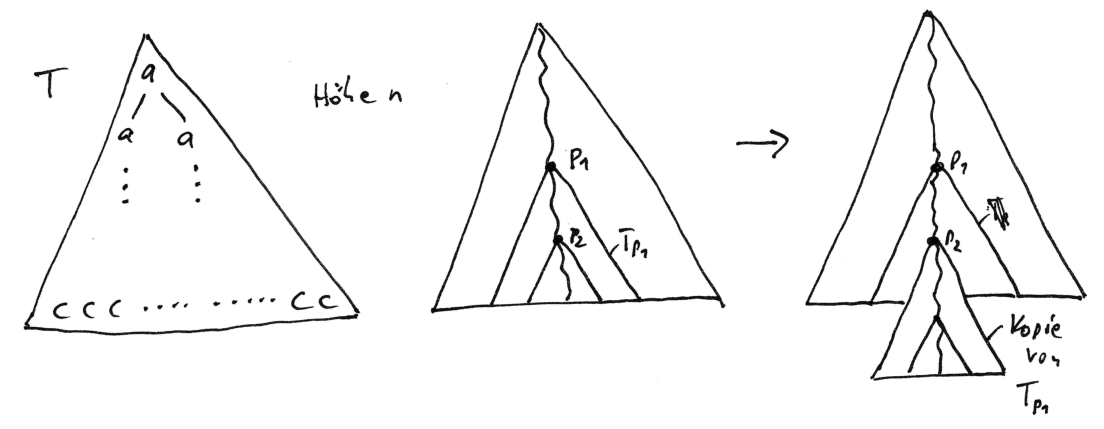
\includegraphics[width=.95\linewidth]{img/t2_5.pdf}
\end{center}

% ===================================================================
\section*{T2.6~ Beispiele für Kontexte}

\begin{itemize}
  \item
    %\paragraph*{Unärer Kontext {\boldmath $C$}, schematisch:}
    Unärer Kontext, schematisch:
    %
    \begin{center}
      \begin{tikzpicture}[%
        node distance=20mm,>=Latex,
        every node/.style={circle,draw=black,thin,fill=black!5,inner sep=.4mm,minimum size=6mm},
        level 1/.style = {sibling distance = 18mm, level distance =  11mm},
        level 2/.style = {sibling distance =  9mm, level distance =  11mm},
        edge from parent/.style = {draw=black, thin, -}%
      ]
        \node (eps) {}
        child {
          node (0) {}
          child {
            node (00) {}
          }
        }
        child {
          node[fill=black!15] (1) {$x$}
        }
        child {
          node (2) {}
          child {
            node (20) {}
          }
        }
        ;
    
        \node [draw=none,fill=none,left=3mm of 0]  {$C$};
      \end{tikzpicture}
    \end{center}
    %
  \item
    Einsetzen:
    %
    \begin{center}
      \begin{tikzpicture}[%
        baseline=-1mm,
        node distance=20mm,>=Latex,
        every node/.style={circle,draw=black,thin,fill=black!2,inner sep=.4mm,minimum size=6mm},
        level 1/.style = {sibling distance = 9mm, level distance =  11mm},
        edge from parent/.style = {draw=black, thin, -}%
      ]
        \node (eps) {}
        child {
          node (0) {}
        }
        child {
          node (1) {}
        }
        ;
    
        \node [draw=none,fill=none,left=11mm of eps]  {Baum $T$};
      \end{tikzpicture}
      \qquad$\leadsto$\qquad
      \begin{tikzpicture}[%
        baseline=-12mm,
        node distance=20mm,>=Latex,
        every node/.style={circle,draw=black,thin,fill=black!5,inner sep=.4mm,minimum size=6mm},
        level 1/.style = {sibling distance = 18mm, level distance =  11mm},
        level 2/.style = {sibling distance =  9mm, level distance =  11mm},
        edge from parent/.style = {draw=black, thin, -}%
      ]
        \node (eps) {}
        child {
          node (0) {}
          child {
            node (00) {}
          }
        }
        child {
          node[fill=black!2] (1) {}
          child {
            node[fill=black!2] (10) {}
          }
          child {
            node[fill=black!2] (11) {}
          }
        }
        child {
          node (2) {}
          child {
            node (20) {}
          }
        }
        ;
    
        \node [draw=none,fill=none,left=5mm of 0]  {Baum $C[T]$};
      \end{tikzpicture}
    \end{center}
    %
    \begin{center}
      \begin{tikzpicture}[%
        baseline=-1mm,
        node distance=20mm,>=Latex,
        every node/.style={circle,draw=black,thin,fill=black!2,inner sep=.4mm,minimum size=6mm},
        level 1/.style = {sibling distance = 9mm, level distance =  11mm},
        edge from parent/.style = {draw=black, thin, -}%
      ]
        \node (eps) {}
        child {
          node[fill=black!15] (0) {$x$}
        }
        child {
          node (1) {}
        }
        ;
    
        \node [draw=none,fill=none,left=11mm of eps]  {Kontext $C'$};
      \end{tikzpicture}
      \qquad$\leadsto$\qquad
      \begin{tikzpicture}[%
        baseline=-12mm,
        node distance=20mm,>=Latex,
        every node/.style={circle,draw=black,thin,fill=black!5,inner sep=.4mm,minimum size=6mm},
        level 1/.style = {sibling distance = 18mm, level distance =  11mm},
        level 2/.style = {sibling distance =  9mm, level distance =  11mm},
        edge from parent/.style = {draw=black, thin, -}%
      ]
        \node (eps) {}
        child {
          node (0) {}
          child {
            node (00) {}
          }
        }
        child {
          node[fill=black!2] (1) {}
          child {
            node[fill=black!15] (10) {$x$}
          }
          child {
            node[fill=black!2] (11) {}
          }
        }
        child {
          node (2) {}
          child {
            node (20) {}
          }
        }
        ;
    
        \node [draw=none,fill=none,left=5mm of 0]  {Kontext $C[C']$};
      \end{tikzpicture}
    \end{center}
    %
    \parII
  \item
    Trivialer Kontext:
    \qquad
    \begin{tikzpicture}[%
      baseline=-1mm,
      node distance=20mm,>=Latex,
      every node/.style={circle,draw=black,thin,fill=black!2,inner sep=.4mm,minimum size=6mm},
      level 1/.style = {sibling distance = 9mm, level distance =  11mm},
      edge from parent/.style = {draw=black, thin, -}%
    ]
      \node[fill=black!15] (eps) {$x$}
      ;
  
      \node [draw=none,fill=none,left=3mm of eps]  {$C_0$};
    \end{tikzpicture}
    \parII
  \item
    Iterierte Kontexte:
    %
    \begin{center}
      \begin{tikzpicture}[%
        baseline=-12mm,
        node distance=20mm,>=Latex,
        every node/.style={circle,draw=black,thin,fill=black!5,inner sep=.4mm,minimum size=6mm},
        level 1/.style = {sibling distance = 21mm, level distance =  11mm},
        level 2/.style = {sibling distance =  9mm, level distance =  11mm},
        edge from parent/.style = {draw=black, thin, -}%
      ]
        \node (eps) {}
        child {
          node (0) {}
          child {
            node (00) {}
          }
        }
        child {
          node[fill=black!2] (1) {}
          child {
            node[fill=black!2] (10) {}
            child {
              node[fill=black!2] (100) {}
            }
          }
          child {
            node[fill=black!15] (11) {$x$}
          }
          child {
            node[fill=black!2] (12) {}
            child {
              node[fill=black!2] (120) {}
            }
          }
        }
        child {
          node (2) {}
          child {
            node (20) {}
          }
        }
        ;
    
        \node [draw=none,fill=none,left=5mm of 0]  {$C^2$};
      \end{tikzpicture}
    \end{center}
\end{itemize}

% ===================================================================
\section*{T2.7~ Illustrationen zum Beweis des Pumping-Lemmas}

\begin{center}
  \parbox{.15\linewidth}{%
    Folie~2.32:%
  }%
  \parbox{.35\linewidth}{%
    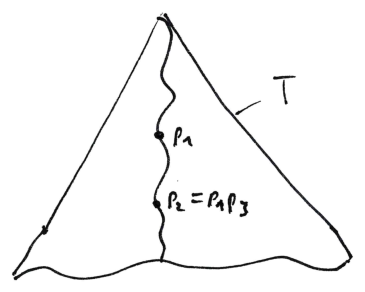
\includegraphics[width=\linewidth]{img/t2_7a.pdf}%
  }%
  \parbox{.15\linewidth}{%
    Folie~2.33:%
  }%
  \parbox{.35\linewidth}{%
    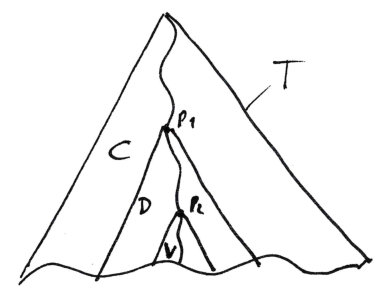
\includegraphics[width=\linewidth]{img/t2_7b.pdf}%
  }%
\end{center}
%
\begin{center}
  \parbox{.15\linewidth}{%
    Folie~2.34:%
  }%
  \parbox{.35\linewidth}{%
    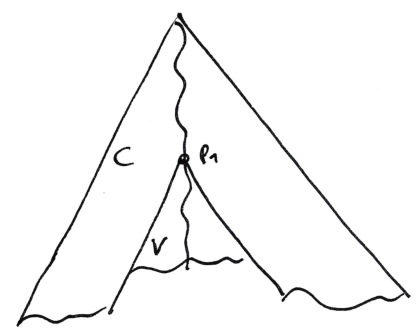
\includegraphics[width=\linewidth]{img/t2_7c.pdf}%
  }%
  \parbox{.15\linewidth}{%
    Folie~2.35:%
  }%
  \parbox{.35\linewidth}{%
    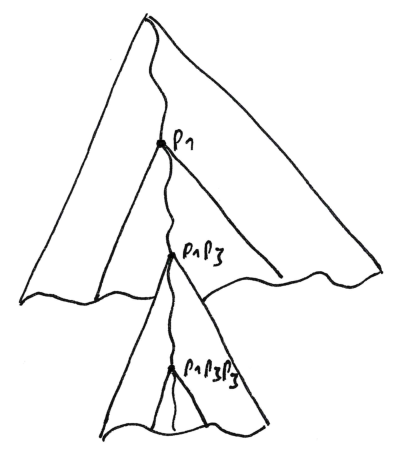
\includegraphics[width=\linewidth]{img/t2_7d.pdf}%
  }%
\end{center}
%
%

\pagebreak
% ===================================================================
\section*{T2.8~ Anwendung des Pumping-Lemmas}

Wir betrachten wieder $L_2 = \{T \mid \text{$T$ ist vollständiger Binärbaum}\}$,
aber diesmal über dem r-Alphabet $\Sigma = \{a/2,\,b/0\}$,
denn einstellige Symbole können in einem vollständigen Binärbaum sowieso nicht vorkommen.

Sei $k \geq 0$ beliebig.
Wir wählen als $T$ den vollständigen Binärbaum der Höhe $k$:
%
\begin{center}
  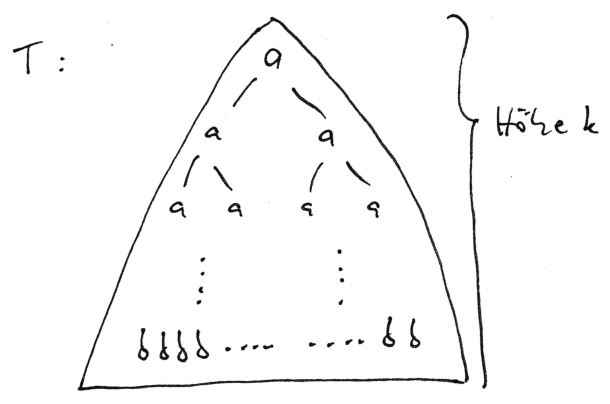
\includegraphics[width=.5\linewidth]{img/t2_8a.pdf}%
\end{center}
%
Sei nun $T=C[D[V]]$ eine Zerlegung von $T$ in Kontexte
$C,D$ und Baum $V$ mit $D$ nichttrivial.
Seien weiterhin
%
\begin{itemize}
  \item
    $p_1$ die Position von $x$ im Kontext $C$;
  \item
    $d_1$ die Tiefe von $p_1$ in $C$, d.\,h.\ $d_1 = |p_1|$;
  \item
    $p_2$ die Position von $x$ im Kontext $D$;
  \item
    $d_2$ die Tiefe von $p_2$ in $D$, d.\,h.\ $d_2 = |p_2| > 0$, da $D$ nichttrivial;
  \item
    $p_3$ eine Blattposition in $V$;
  \item
    $d_3$ die Höhe von $V$ (und damit die Tiefe aller Blätter, denn $T$ ist vollständig).
\end{itemize}
%
\begin{center}
  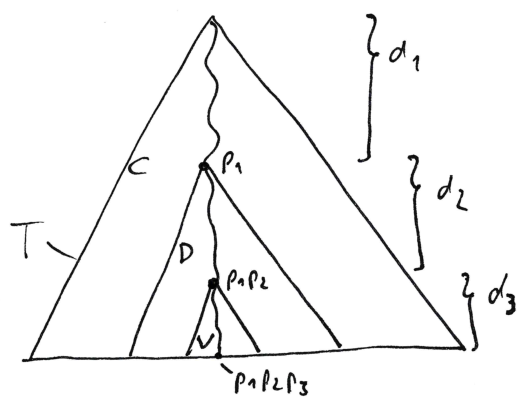
\includegraphics[width=.5\linewidth]{img/t2_8b.pdf}%
\end{center}
%
Weil $T$ vollständig ist, haben alle Pfade in $T$ die Länge $k = d_1+d_2+d_3$.

Wir wählen nun $i=2$ und betrachten den "`gepumpten"' Baum $C[D^2[V]]$:
%
\begin{center}
  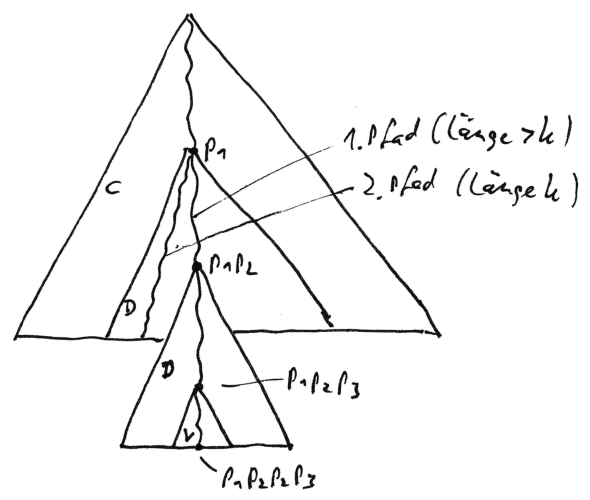
\includegraphics[width=.5\linewidth]{img/t2_8c.pdf}%
\end{center}
%
In diesem Baum gibt es einen Pfad der Länge $d_1+2d_2+d_3 > k$, nämlich zur Position $p_1p_2p_2p_3$.
Da $T$ vollständig ist, hat $p_1$ ein Kind, das nicht auf diesem Pfad liegt und dessen Teilbaum
also nicht vom Pumpen betroffen ist.
Deshalb gibt es in $C[D^2[V]]$ auch einen Pfad der Länge $k$,
woraus folgt, dass $C[D^2[V]]$ nicht vollständig ist und damit auch nicht zu $L_2$ gehören kann.

\paragraph*{Anmerkung.} Abpumpen, d.\,h.\ die Wahl von $i=0$, funktioniert hier nicht,
denn es ist nicht ausgeschlossen, dass $C$ der triviale Kontext ist.
In diesem Fall ist $C[D^0[V]] = C[V] = V$ nach wie vor ein vollständiger Binärbaum,
gehört also zu $L_2$.

% ===================================================================
\section*{T2.9~ Anwendung Nerode-Rechtskongruenz für Baumsprachen}

Wir betrachten $L_1 = \{T \mid \text{$T$ hat gerade Höhe}\}$
über dem r-Alphabet $\Sigma = \{a/2,\,b/1\,c/0\}$.
Um zu zeigen, dass $L_1$ nicht NEBA-erkennbar ist,
müssen wir eine Folge $(T_n)_{n \geq 1}$ von Bäumen über $\Sigma$ finden,
so dass $T_n \not\sim_{L_1} T_k$ für alle $1 \leq n < k$ gilt.

Wir wählen diese Bäume so, dass $T_n$ der Pfad $b(b(b\cdots (b(c)) \cdots ))$ der Höhe $2n$ ist.
Seien nun $n,k$ mit $1 \leq n < k$ beliebig.
Um $T_n \not\sim_{L_1} T_k$ zu zeigen,
betrachten wir den Kontext $C = a(b(x)T_k)$:
%
\vspace*{-\baselineskip}
\begin{center}
  \begin{tikzpicture}[%
    node distance=20mm,>=Latex,
    every node/.style={circle,draw=black,thin,fill=black!5,inner sep=.4mm,minimum size=6mm},
    level 1/.style = {sibling distance = 18mm, level distance =  8mm},
    level 2/.style = {sibling distance =  9mm, level distance = 10mm},
    edge from parent/.style = {draw=black, thin, -}%
  ]
    \node (eps) {$a$}
    child {
      node (0) {$b$}
      child {
        node[fill=black!15] (00) {$x$}
      }
    }
    child {
      node (1) {$b$}
      child {
        node (10) {$b$}
          child {
            node[draw=none,fill=none,inner sep=1mm] (100) {$\vdots$}
              child {
                node (1000) {$b$}
                  child {
                    node (10000) {$c$}
                  }
              }
          }
      }
    }
    ;

    \node [draw=none,fill=none,left=3mm of 0]  {$C$};
    
    \node [rectangle,rounded corners,fill=none,inner sep=1mm,fit=(1) (10000)] (Tk) {};
    
    \node [draw=none,fill=none,right=0mm of Tk] {$=T_k$~ (Höhe $2k$)};
  \end{tikzpicture}
\end{center}
%
Da $1 \leq n < k$, hat $C$ die Höhe $2k+1$. Nun gilt:
%
\begin{itemize}
  \item
    $C[T_n]$ hat ebenfalls Höhe $2k+1$, da die Höhe von $T_n$ um mindestens 2 kleiner ist
    als die Höhe von $T_k$ und damit in $C[T_n]$ der linke Pfad nicht länger werden kann als der rechte.
  \item 
    $C[T_k]$ hat jedoch Höhe $2k+2$, da der linker Pfad um 1 länger ist als der rechte
    (denn das linke Vorkommen von $T_k$ beginnt eine Ebene tiefer als das rechte).
\end{itemize}
%
Damit ist $C[T_n] \notin L_1$ und $C[T_k] \in L_1$, woraus wie gewünscht $T_n \not\sim_{L_1} T_k$ folgt.

% ===================================================================
\section*{T2.10~ Mächtigkeit von DETDBAs}

\textsfbf{Lemma~2.14.}~
Die erkennbare Baumsprache $L=\{a(bc),a(cb)\}$ wird von keinem DETDBA erkannt.

\parII
\begin{beweis}
  Angenommen, es gebe einen DETDBA $\Amc = (Q,\Sigma,\Delta,I)$ mit $L(\Amc) = L$.
  Wegen des Determinismus gibt es nur einen einzigen Anfangszustand $q_I$
  und genau einen Übergang $(a,q_I) \to (q_1,q_2)$ mit $(a,q_I)$ auf der linken Seite.
%  ("`höchstens einen"' wegen Determinismus; "`mindestens einen"' wegen $a(bc) \in L$).
  Da $a(bc),a(cb) \in L$, muss $\Delta$ auch die folgenden Übergänge enthalten:
  %
  \begin{xalignat*}{2}
    (b,q_1) & \to () & (c,q_1) & \to () \\
    (c,q_2) & \to () & (b,q_2) & \to ()
  \end{xalignat*}
  %
  Also hat \Amc auch einen erfolgreichen Run auf $a(bb)$;
  also $a(bb) \in L$, Widerspruch zur Definition von $L$.
  \qedhere
\end{beweis}

\goodbreak
% ===================================================================
\section*{T2.11~ Korrektheit des Algorithmus fürs Leerheitsproblem}

\textsfbf{Behauptung:}~ $L(\Amc) = \emptyset$ gdw.\ $R \cap F = \emptyset$.

\parII
\begin{beweis}
  Wir zeigen beide Richtungen per Kontraposition.
  %
  \begin{description}
    \item[{\boldmath "`$\Leftarrow$"'}]
      Sei $L(\Amc) \neq \emptyset$.
      Dann gibt es einen Baum $T=(P,t) \in L(\Amc)$.
      Sei $r$ ein erfolgreicher Run von \Amc auf $T$.
      Man zeigt leicht per Induktion über die Höhe,
      dass für alle Positionen $p \in P$ gilt: $r(p) \in R$.
      Also gilt insbesondere $r(\varepsilon) \in R$.
      Da auch $r(\varepsilon) \in F$ gilt ($r$ ist erfolgreich),
      ist $R \cap F \neq \emptyset$.
    \item[{\boldmath "`$\Rightarrow$"'}]
      Gelte $R \cap F \neq \emptyset$ und sei $q \in R \cap F$.
      Um zu zeigen, dass $L(\Amc) \neq \emptyset$ gilt,
      konstruieren wir einen Baum $T$
      und einen Run $r$ von \Amc auf $T$
      mit $r(\varepsilon) = q$ (woraus mit $q \in R \cap F$ folgt,
      dass $r$ erfolgreich ist).
      Wir definieren $P,t,r$ iterativ wie folgt.
      %
      \begin{enumerate}
        \item[(1)]
          Sei $a(q_1,\dots,q_m) \to q$ der eindeutig bestimmte Übergang,
          der zu $q \in R$ geführt hat. Setze:
          %
          \begin{itemize}
            \item
              $P = \{\varepsilon,1,\dots,m\}$
            \item
              $t(\varepsilon)=a$
            \item 
              $r(\varepsilon) = q$, $r(1)=q_1$, \dots, $r(m) = q_m$
          \end{itemize}
        \item[(2)]
          Solange es ein $p \neq \varepsilon$ gibt
          mit $r(p) = q'$ definiert, aber $t(p)$ noch nicht definiert, tue folgendes:
          
          Sei $a'(q'_1,\dots,q'_n) \to q'$ der eindeutig bestimmte Übergang,
          der zu $q' \in R$ geführt hat. Setze:
          %
          \begin{itemize}
            \item
              $P = P \cup \{pj \mid j = 1,\dots,n\}$
            \item
              $t(p)=a'$
            \item 
              $r(p_1)=q'_1$, \dots, $r(p_n) = q'_n$
          \end{itemize}
      \end{enumerate}
      %
      Dieser Prozess endet nach endlich vielen Anwendungen von~(2),
      weil auf jedem Pfad von $r$ kein Zustand doppelt auftreten kann, denn nach Konstruktion gilt:
      %
      \begin{quote}
        Wenn $r(p) = \widehat q$ und $r(pi) = \widehat q'$, dann ist $\widehat q$ später als $\widehat q'$
        zu $R$ hinzugefügt worden.
      \end{quote}
      %
      Also ist $T=(P,t)$ endlich.
      Außerdem ist $r$ ein Run, denn die Übergangsrelation $\Delta$ wird nach Konstruktion respektiert.
      (Erfolgreich ist $r$, weil $r(\varepsilon) = q \in R \cap F$.)
      Folglich ist $L(\Amc) \neq \emptyset$.
      \qedhere
  \end{description}
\end{beweis}

% ===================================================================
\section*{T2.12~ Beispiele für Hecken und Bäume}

Sei $\Sigma = \{a,b,c\}$.
%
\begin{itemize}
  \item 
    $\varepsilon$ ist eine Hecke.
  \item
    Dann ist auch $a = a()$ ein Baum:
    \qquad
    %
    \begin{tikzpicture}[%
      baseline=-2pt,
      node distance=20mm,>=Latex,
      every node/.style={circle,draw=black,thin,fill=black!5,inner sep=.4mm,minimum size=6mm},
    ]
      \node (eps) {$a$};
    \end{tikzpicture}
    \parII
  \item
    Dann ist auch $aa$ eine Hecke:
    \qquad
    %
    \begin{tikzpicture}[%
      baseline=-2pt,
      node distance=20mm,>=Latex,
      every node/.style={circle,draw=black,thin,fill=black!5,inner sep=.4mm,minimum size=6mm},
    ]
      \node (eps)  {$a$};
      \node[right=4mm of eps] (eps2) {$a$};
    \end{tikzpicture}
    \parII
  \item
    Dann ist auch $b(aa)$ ein Baum:
    \qquad
    %
    \begin{tikzpicture}[%
      baseline=-2pt,
      node distance=20mm,>=Latex,
      every node/.style={circle,draw=black,thin,fill=black!5,inner sep=.4mm,minimum size=6mm},
      level 1/.style = {sibling distance = 10mm, level distance =  8mm},
      edge from parent/.style = {draw=black, thin, -}%
    ]
      \node (eps) {$b$}
        child {
          node (0) {$a$}
        }
        child {
          node (1) {$a$}
        }
      ;
    \end{tikzpicture}
    \parII
  \item
    Dann ist auch $ab(aa)c$ eine Hecke:
    \qquad
    %
    \begin{tikzpicture}[%
      baseline=-2pt,
      node distance=20mm,>=Latex,
      every node/.style={circle,draw=black,thin,fill=black!5,inner sep=.4mm,minimum size=6mm},
      level 1/.style = {sibling distance = 10mm, level distance =  8mm},
      edge from parent/.style = {draw=black, thin, -}%
    ]
      \node (eps1) {$a$};
      \node[right=6mm of eps1] (eps2) {$b$}
        child {
          node (0) {$a$}
        }
        child {
          node (1) {$a$}
        }
      ;
      \node[right=6mm of eps2] (eps3) {$c$};
    \end{tikzpicture}
    \parII
  \item
    Dann ist auch $a(ab(aa)c)$ ein Baum:
    \qquad
    %
    \begin{tikzpicture}[%
      baseline=-2pt,
      node distance=20mm,>=Latex,
      every node/.style={circle,draw=black,thin,fill=black!5,inner sep=.4mm,minimum size=6mm},
      level 1/.style = {sibling distance = 12mm, level distance = 10mm},
      level 2/.style = {sibling distance = 10mm, level distance = 10mm},
      edge from parent/.style = {draw=black, thin, -}%
    ]
      \node (eps) {$a$}
        child {
          node (0) {$a$}
        }
        child {
          node (1) {$b$}
          child {
            node (10) {$a$}
          }
          child {
            node (11) {$a$}
          }
        }
        child {
          node (2) {$c$}
        }
      ;
    \end{tikzpicture}
\end{itemize}

\par\vspace*{\baselineskip}
Auch $a(c(b)cb(ab))$ ist ein Baum:
\qquad
%
\begin{tikzpicture}[%
  baseline=-2pt,
  node distance=20mm,>=Latex,
  every node/.style={circle,draw=black,thin,fill=black!5,inner sep=.4mm,minimum size=6mm},
  level 1/.style = {sibling distance = 12mm, level distance = 10mm},
  level 2/.style = {sibling distance = 10mm, level distance = 10mm},
  edge from parent/.style = {draw=black, thin, -}%
]
  \node (eps) {$a$}
    child {
      node (0) {$c$}
      child {
        node (00) {$b$}
      }
    }
    child {
      node (1) {$c$}
    }
    child {
      node (2) {$b$}
      child {
        node (20) {$a$}
      }
      child {
        node (21) {$b$}
      }
    }
  ;
\end{tikzpicture}

% ===================================================================
\section*{T2.13~ Problem mit NEBAs auf Bäumen ohne Stelligkeit}

Sei $\Sigma = \{a\}$, wobei $a$ ohne Stelligkeit ist.
Wir betrachten die Sprache $L$ aller Bäume mit Höhe 1 über $\Sigma$,
also $L = \{a(a), a(aa), a(aaa), \dots\}$.
Wenn wir nun einen (Bottom-up-)Baumautomaten $\Amc = (Q,\Sigma,\Delta,F)$
mit $L(\Amc)=L$ konstruieren wollen,
dann sollte dieser zwei Zustände $q_0,q_1$ haben,
um zwischen den zwei Ebenen zu unterscheiden;
außerdem müsste er für jedes $k \geq 1$ einen Übergang
\[
   a(\underbrace{q_0,\dots,q_0}_{k\text{-mal}}) \to q_1
\]
haben -- damit wäre aber $\Delta$ nicht mehr endlich.

Abhilfe kann man schaffen, indem man eine reguläre Sprache $R \subseteq Q^*$ benutzt,
die genau die unendlich vielen Folgen $q_0,\dots,q_0$ beschreibt.
Wenn man $R$ mittels eines regulären Ausdrucks beschreibt,
erhält man hier einen einzigen Übergang, nämlich
\[
  a(q_0^+) \to q_1,
\]
wobei $q_0^+$ die übliche Abkürzung für $q_0q_0^*$ ist
($q_0^*$ genügt nicht, denn oben ist $k = 0$ nicht erlaubt).

% ===================================================================
\section*{T2.14~ Beispiel-NEHA}

Wir beginnen mit einem Beispiel für den tiefsten gemeinsamen Vorgänger (tgV)
zweier Positionen $p_1,p_2$. Intuitiv gesprochen ist $\textsf{tgV}(p_1,p_2)$
die Stelle, an der sich die zwei Pfade zu $p_1$ bzw.\ $p_2$ trennen:
%
\begin{center}
  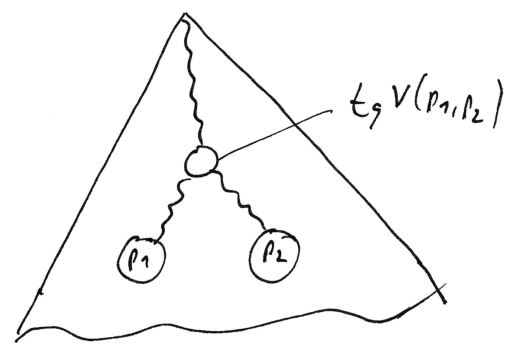
\includegraphics[width=.4\linewidth]{img/t2_14.pdf}%
\end{center}
%
Eine solche Position existiert immer, denn je zwei Pfade haben mindestens
die Position $\varepsilon$ gemeinsam.

Wenn wir untenstehenden Baum betrachten (nur die Positionen),
dann gilt Nebenstehendes.
\parII
\hspace*{10mm}
\parbox{.5\linewidth}{%
  \begin{tikzpicture}[%
    baseline=-2pt,
    node distance=20mm,>=Latex,
    every node/.style={circle,draw=black,thin,fill=black!5,inner sep=.4mm,minimum size=7mm},
    level 1/.style = {sibling distance = 30mm, level distance =  6mm},
    level 2/.style = {sibling distance = 13mm, level distance = 10mm},
    level 3/.style = {sibling distance = 10mm, level distance = 10mm},
    edge from parent/.style = {draw=black, thin, -}%
  ]
    \node (eps) {$\varepsilon$}
      child {
        node (1) {$1$}
        child {
          node (11) {$11$}
        }
        child {
          node (12) {$12$}
        }
        child {
          node (13) {$13$}
            child {
              node (131) {$131$}
            }
            child {
              node (132) {$132$}
            }
        }
      }
      child {
        node (2) {$2$}
      }
    ;
  \end{tikzpicture}%
}%
\parbox{.3\linewidth}{
  \begin{alignat*}{2}
    \textsf{tgV}(131,{}& 132) & & = 13 \\
    \textsf{tgV}(132,{}& 12)  & & = 1 \\
    \textsf{tgV}(132,{}& 2)   & & = \varepsilon
  \end{alignat*}
}

\parIII
Nun betrachten wir die Sprache
\begin{align*}
  L = \{T = (P,t) \mid{} & \text{es gibt~} p_1,p_2 \in P \text{~mit~} t(p_1) = t(p_2) = b \text{~und~} t(\text{tgV}(p_1,p_2)) = c\}
\end{align*}
und den folgenden Baum $L$ über dem Alphabet $\Sigma = \{a,b,c\}$ (ohne Stelligkeit).
%
\begin{center}
  \begin{tikzpicture}[%
    baseline=-2pt,
    node distance=20mm,>=Latex,
    every node/.style={circle,draw=black,thin,fill=black!5,inner sep=.4mm,minimum size=7mm},
    level 1/.style = {sibling distance = 34mm, level distance =  6mm},
    level 2/.style = {sibling distance = 13mm, level distance = 10mm},
    level 3/.style = {sibling distance = 10mm, level distance = 10mm},
    edge from parent/.style = {draw=black, thin, -}%
  ]
    \node (eps) {$a$}
      child {
        node[fill=black!20] (0) {$c$}
        child {
          node (11) {$a$}
        }
        child {
          node[fill=black!20] (12) {$b$}
        }
        child {
          node (13) {$a$}
            child {
              node (131) {$c$}
            }
            child {
              node[fill=black!20] (132) {$b$}
            }
        }
      }
      child {
        node (2) {$b$}
        child {
          node (21) {$a$}
          child {
            node (211) {$a$}
          }
        }
      }
    ;
  \end{tikzpicture}%
\end{center}
%
An den hervorgehobenen Positionen erkennt man, dass $T \in L$.

\parIII
Der NEHA \Amc von Folie~2.79 hat folgenden erfolgreichen Run auf $T$:
%
\begin{center}
  \begin{tikzpicture}[%
    baseline=-2pt,
    node distance=20mm,>=Latex,
    every node/.style={circle,draw=black,thin,fill=black!5,inner sep=.4mm,minimum size=7mm},
    level 1/.style = {sibling distance = 34mm, level distance =  6mm},
    level 2/.style = {sibling distance = 13mm, level distance = 10mm},
    level 3/.style = {sibling distance = 10mm, level distance = 10mm},
    edge from parent/.style = {draw=black, thin, -}%
  ]
    \node (eps) {$q_c$}
      child {
        node[fill=black!20] (0) {$q_c$}
        child {
          node (11) {$q_0$}
        }
        child {
          node[fill=black!20] (12) {$q_b$}
        }
        child {
          node (13) {$q_b$}
            child {
              node (131) {$q_0$}
            }
            child {
              node[fill=black!20] (132) {$q_b$}
            }
        }
      }
      child {
        node (2) {$q_b$}
        child {
          node (21) {$q_0$}
          child {
            node (211) {$q_0$}
          }
        }
      }
    ;
  \end{tikzpicture}%
\end{center}

\pagebreak
% ===================================================================
\section*{T2.15~ Beispielableitung in DTD}

Wir betrachten die durch folgende erweiterte kontextfreie Grammatik
gegebene DTD.
%
\begin{center}
  \begin{tabular}{@{}lcl@{}}
    \texttt{conference} & $\to$ & $\texttt{track}^+ + (\texttt{session}~(\texttt{break} + \varepsilon))^+$ \\
    \texttt{track}      & $\to$ & $(\texttt{session}~(\texttt{break} + \varepsilon))^+$                    \\
    \texttt{session}    & $\to$ & $\texttt{chair}~ \texttt{talk}^+$                                        \\
    \texttt{talk}       & $\to$ & $(\texttt{title}~\texttt{authors}) + (\texttt{title}~\texttt{speaker})$  \\
    \texttt{chair}      & $\to$ & $\texttt{DATA}$                                                          \\
    \dots               &       &                                                                          \\
    \texttt{title}      & $\to$ & $\texttt{DATA}$
  \end{tabular}
\end{center}
%
Eine mögliche Ableitung beginnt wie folgt.
%
\begin{itemize}
  \item
    Beginne mit dem Startsymbol:
    %
    \begin{center}
      \begin{tikzpicture}[%
        baseline=-2pt,
        node distance=20mm,>=Latex,
        every node/.style={ellipse,draw=black,thin,fill=black!5,inner sep=.6mm},
      ]
        \node (eps) {{\small \texttt{conference}}}
        ;
      \end{tikzpicture}
    \end{center}
    \parII
  \item
    Wende Regel 1 auf diesen Knoten an:
    %
    \begin{center}
      \begin{tikzpicture}[%
        baseline=-2pt,
        node distance=20mm,>=Latex,
        every node/.style={ellipse,draw=black,thin,fill=black!5,inner sep=.6mm},
        level 1/.style = {sibling distance = 54mm, level distance = 10mm},
        edge from parent/.style = {draw=black, thin, -}%
      ]
        \node (eps) {{\small \texttt{conference}}}
          child {
            node (1) {{\small \texttt{track}}}
          }
          child {
            node (2) {{\small \texttt{track}}}
          }
        ;
      \end{tikzpicture}
    \end{center}
    \parII
  \item
    Wende Regel 2 auf das linke \texttt{track}-Blatt an:
    %
    \begin{center}
      \begin{tikzpicture}[%
        baseline=-2pt,
        node distance=20mm,>=Latex,
        every node/.style={ellipse,draw=black,thin,fill=black!5,inner sep=1mm},
        level 1/.style = {sibling distance = 54mm, level distance = 10mm},
        level 2/.style = {sibling distance = 24mm, level distance = 10mm},
        edge from parent/.style = {draw=black, thin, -}%
      ]
        \node (eps) {{\small \texttt{conference}}}
          child {
            node (1) {{\small \texttt{track}}}
            child {
              node (11) {{\small \texttt{session}}}
            }
            child {
              node (12) {{\small \texttt{break}}}
            }
            child {
              node (13) {{\small \texttt{session}}}
            }
          }
          child {
            node (2) {{\small \texttt{track}}}
          }
        ;
      \end{tikzpicture}
    \end{center}
    \parII
  \item
    Wende Regel 6 auf das \texttt{break}-Blatt an:
    %
    \begin{center}
      \begin{tikzpicture}[%
        baseline=-2pt,
        node distance=20mm,>=Latex,
        every node/.style={ellipse,draw=black,thin,fill=black!5,inner sep=1mm},
        level 1/.style = {sibling distance = 54mm, level distance = 10mm},
        level 2/.style = {sibling distance = 24mm, level distance = 10mm},
        edge from parent/.style = {draw=black, thin, -}%
      ]
        \node (eps) {{\small \texttt{conference}}}
          child {
            node (1) {{\small \texttt{track}}}
            child {
              node (11) {{\small \texttt{session}}}
            }
            child {
              node (12) {{\small \texttt{break}}}
              child {
                node (121) {{\small \texttt{DATA}}}
              }
            }
            child {
              node (13) {{\small \texttt{session}}}
            }
          }
          child {
            node (2) {{\small \texttt{track}}}
          }
        ;
      \end{tikzpicture}
    \end{center}
    %
    \parII
    Auf das neu entstandene \texttt{DATA}-Blatt ist nun keine Regel mehr anwendbar.
    \parII
    \goodbreak
  \item
    Wende Regel 3 auf das linke \texttt{session}-Blatt an:
    %
    \begin{center}
      \begin{tikzpicture}[%
        baseline=-2pt,
        node distance=20mm,>=Latex,
        every node/.style={ellipse,draw=black,thin,fill=black!5,inner sep=1mm},
        level 1/.style = {sibling distance = 54mm, level distance = 10mm},
        level 2/.style = {sibling distance = 34mm, level distance = 10mm},
        level 3/.style = {sibling distance = 20mm, level distance = 10mm},
        edge from parent/.style = {draw=black, thin, -}%
      ]
        \node (eps) {{\small \texttt{conference}}}
          child {
            node (1) {{\small \texttt{track}}}
            child {
              node (11) {{\small \texttt{session}}}
              child {
                node (111) {{\small \texttt{session}}}
              }
              child {
                node (112) {{\small \texttt{talk}}}
              }
              child {
                node [right=2mm of 112] (113) {{\small \texttt{talk}}}
              }
            }
            child {
              node (12) {{\small \texttt{break}}}
              child {
                node (121) {{\small \texttt{DATA}}}
              }
            }
            child {
              node [right=5mm of 12] (13) {{\small \texttt{session}}}
            }
          }
          child {
            node (2) {{\small \texttt{track}}}
          }
        ;
      \end{tikzpicture}
    \end{center}
    \parII
  \item
    (usw.)
\end{itemize}
%
\parIII
Es wird solange jeweils eine Regel auf ein Blatt angewendet,
bis keine Regel mehr anwendbar ist.

% ===================================================================
\section*{T2.16~ Beispiele nicht lokaler Sprachen}

\textsfbf{Beispiel 1.}
\[
  L_1 = \{a(b(ccc)b(cc)),\,a(b(cc)b(c))\},
\]
d.\,h.\ $L_1$ besteht genau aus den Bäumen
%
\begin{center}
  \begin{tikzpicture}[%
    baseline=-2pt,
    node distance=20mm,>=Latex,
    every node/.style={circle,draw=black,thin,fill=black!5,inner sep=.4mm,minimum size=6mm},
    level 1/.style = {sibling distance = 32mm, level distance =  6mm},
    level 2/.style = {sibling distance =  9mm, level distance = 10mm},
    edge from parent/.style = {draw=black, thin, -}%
  ]
    \node (eps) {$a$}
      child {
        node (1) {$b$}
        child {
          node (11) {$c$}
        }
        child {
          node (12) {$c$}
        }
        child {
          node (13) {$c$}
        }
      }
      child {
        node (2) {$b$}
        child {
          node (21) {$c$}
        }
        child {
          node (22) {$c$}
        }
      }
    ;
  \end{tikzpicture}%
  \hspace*{20mm}%
  \begin{tikzpicture}[%
    baseline=-2pt,
    node distance=20mm,>=Latex,
    every node/.style={circle,draw=black,thin,fill=black!5,inner sep=.4mm,minimum size=6mm},
    level 1/.style = {sibling distance = 32mm, level distance =  6mm},
    level 2/.style = {sibling distance =  9mm, level distance = 10mm},
    edge from parent/.style = {draw=black, thin, -}%
  ]
    \node (eps) {$a$}
      child {
        node (1) {$b$}
        child {
          node (11) {$c$}
        }
        child {
          node (12) {$c$}
        }
      }
      child {
        node (2) {$b$}
        child {
          node (21) {$c$}
        }
        child {
          node (22) {$c$}
        }
        child {
          node (23) {$c$}
        }
      }
    ;
  \end{tikzpicture}%
\end{center}
%
$L_1$ ist nicht lokal, denn wenn $L_1$ von einer DTD erzeugt würde,
dann müsste diese DTD auch die folgenden Bäume erzeugen:
%
\begin{center}
  \begin{tikzpicture}[%
    baseline=-2pt,
    node distance=20mm,>=Latex,
    every node/.style={circle,draw=black,thin,fill=black!5,inner sep=.4mm,minimum size=6mm},
    level 1/.style = {sibling distance = 32mm, level distance =  6mm},
    level 2/.style = {sibling distance =  9mm, level distance = 10mm},
    edge from parent/.style = {draw=black, thin, -}%
  ]
    \node (eps) {$a$}
      child {
        node (1) {$b$}
        child {
          node (11) {$c$}
        }
        child {
          node (12) {$c$}
        }
      }
      child {
        node (2) {$b$}
        child {
          node (21) {$c$}
        }
        child {
          node (22) {$c$}
        }
      }
    ;
  \end{tikzpicture}%
  \hspace*{20mm}%
  \begin{tikzpicture}[%
    baseline=-2pt,
    node distance=20mm,>=Latex,
    every node/.style={circle,draw=black,thin,fill=black!5,inner sep=.4mm,minimum size=6mm},
    level 1/.style = {sibling distance = 32mm, level distance =  6mm},
    level 2/.style = {sibling distance =  9mm, level distance = 10mm},
    edge from parent/.style = {draw=black, thin, -}%
  ]
    \node (eps) {$a$}
      child {
        node (1) {$b$}
        child {
          node (11) {$c$}
        }
        child {
          node (12) {$c$}
        }
        child {
          node (13) {$c$}
        }
      }
      child {
        node (2) {$b$}
        child {
          node (21) {$c$}
        }
        child {
          node (22) {$c$}
        }
        child {
          node (23) {$c$}
        }
      }
    ;
  \end{tikzpicture}%
\end{center}
%
Man kann also mit DTDs nicht in Tiefe $\geq 2$ zählen.
Für unser Konferenz-Beispiel heißt das, dass man z.\,B.\ keine DTD schreiben kann,
die erfordert, dass alle Konferenzen genau 5 Vorträge haben.

\parII
\textsfbf{Beispiel 2.}
\[
  L_2 = \{a(b(cd)),\,a'(b(dc))\},
\]
d.\,h.\ $L_2$ besteht genau aus den Bäumen
%
\begin{center}
  \begin{tikzpicture}[%
    baseline=-2pt,
    node distance=20mm,>=Latex,
    every node/.style={circle,draw=black,thin,fill=black!5,inner sep=.4mm,minimum size=6mm},
    level 1/.style = {sibling distance = 32mm, level distance =  8mm},
    level 2/.style = {sibling distance =  9mm, level distance =  8mm},
    edge from parent/.style = {draw=black, thin, -}%
  ]
    \node (eps) {$a$}
      child {
        node (1) {$b$}
        child {
          node (11) {$c$}
        }
        child {
          node (12) {$d$}
        }
      }
    ;
  \end{tikzpicture}%
  \hspace*{20mm}%
  \begin{tikzpicture}[%
    baseline=-2pt,
    node distance=20mm,>=Latex,
    every node/.style={circle,draw=black,thin,fill=black!5,inner sep=.4mm,minimum size=6mm},
    level 1/.style = {sibling distance = 32mm, level distance =  8mm},
    level 2/.style = {sibling distance =  9mm, level distance =  8mm},
    edge from parent/.style = {draw=black, thin, -}%
  ]
    \node (eps) {$a'$}
      child {
        node (1) {$b$}
        child {
          node (11) {$d$}
        }
        child {
          node (12) {$c$}
        }
      }
    ;
  \end{tikzpicture}%
\end{center}
%
$L_2$ ist nicht lokal, denn wenn $L_2$ von einer DTD erzeugt würde, dann müsste diese DTD
auch die folgenden Bäume erzeugen:
%
\begin{center}
  \begin{tikzpicture}[%
    baseline=-2pt,
    node distance=20mm,>=Latex,
    every node/.style={circle,draw=black,thin,fill=black!5,inner sep=.4mm,minimum size=6mm},
    level 1/.style = {sibling distance = 32mm, level distance =  8mm},
    level 2/.style = {sibling distance =  9mm, level distance =  8mm},
    edge from parent/.style = {draw=black, thin, -}%
  ]
    \node (eps) {$a$}
      child {
        node (1) {$b$}
        child {
          node (11) {$d$}
        }
        child {
          node (12) {$c$}
        }
      }
    ;
  \end{tikzpicture}%
  \hspace*{20mm}%
  \begin{tikzpicture}[%
    baseline=-2pt,
    node distance=20mm,>=Latex,
    every node/.style={circle,draw=black,thin,fill=black!5,inner sep=.4mm,minimum size=6mm},
    level 1/.style = {sibling distance = 32mm, level distance =  8mm},
    level 2/.style = {sibling distance =  9mm, level distance =  8mm},
    edge from parent/.style = {draw=black, thin, -}%
  ]
    \node (eps) {$a'$}
      child {
        node (1) {$b$}
        child {
          node (11) {$c$}
        }
        child {
          node (12) {$d$}
        }
      }
    ;
  \end{tikzpicture}%
\end{center}
%
Man kann also mit DTDs keine Abhängigkeiten modellieren, die sich über mehrere Ebenen erstrecken,
wie hier z.\,B.: "`bei den Enkeln von $a$ kommt $c$ vor $d$, aber bei den Enkeln von $a'$ ist es anders herum."'
Bezogen auf das Konferenzbeispiel kann man z.\,B.\ mit einer DTD nicht fordern,
dass in Informatik-Konferenzen ($a$) die Publikation ($c$) vor dem Vortrag ($d$) erscheint,
während die Reihenfolge bei Mathematik-Konferenzen ($a'$) umgekehrt ist.

% ===================================================================
\section*{T2.17~ Beispiel für nicht deterministischen regulären Ausdruck}

Der reguläre Ausdruck (RA) $r = ab + ac$ ist nicht deterministisch:
Mittels Nummerieren der Buchstaben erhalten wir $r' = a_1b_1 + a_2c_1$.
Nun sind aber $a_1b_1,a_2c_1 \in L(r')$ (wenn man $u = \varepsilon$, $v=b_1$ und $w=c_1$ wählt),
was Definition~2.28 verletzt.

Es ist aber leicht zu sehen, dass der RA $a(b+c)$
äquivalent zu $r$ ist. Dieser ist trivialerweise deterministisch,
denn jedes Zeichen kommt darin nur einmal vor.

Daraus folgt, dass die Zeile 
%
\begin{center}
  \texttt{talk} ~$\to$~ $(\texttt{title}~\texttt{authors}) + (\texttt{title}~\texttt{speaker})$
\end{center}
%
aus der Beispiel-DTD (Folie~2.86) zwar kein zulässiges Inhaltsmodell enthält,
man sie aber äquivalent mit deterministischem RA so umschreiben kann, dass sie zulässig wird:
%
\begin{center}
  \texttt{talk} ~$\to$~ $\texttt{title}~(\texttt{authors} + \texttt{speaker})$
\end{center}
%


% ===================================================================
% ===================================================================
% ===================================================================
\part[Endliche Automaten auf unendlichen Wörtern]{Endliche Automaten \\ auf unendlichen Wörtern}

% ===================================================================
\section*{T3.1~ Produktkonstruktion für NEAs ist für NBAs nicht korrekt}

Sei $\Sigma = \{a,b\}$. Wir betrachten folgende \textsfbf{NEAs} $\Amc_1,\Amc_2$.
%
\begin{center}
  \begin{tikzpicture}[%
    node distance=20mm,>=Latex,
    initial text="", initial where=below left,
    every state/.style={draw=black,thin,fill=black!5,inner sep=1mm,minimum size=6mm},
    accepting/.style={double distance=1.5pt, double=white},
    every edge/.style={draw=black,thin}
  ]
    \node[state,initial]   (q0) {$q_0$};
    \node[state,accepting] (q1) [right of=q0] {$q_1$};
    \node[above left=-2mm and 6mm of q0] {$\Amc_1$};
    
    \path[->] (q0) edge [bend left=15] node [above] {$a$} (q1)
              (q1) edge [bend left=15] node [below] {$a,b$} (q0);
  \end{tikzpicture}
  \qquad
  \begin{tikzpicture}[%
    node distance=20mm,>=Latex,
    initial text="", initial where=below left,
    every state/.style={draw=black,thin,fill=black!5,inner sep=1mm,minimum size=6mm},
    accepting/.style={double distance=1.5pt, double=white},
    every edge/.style={draw=black,thin}
  ]
    \node[state,initial,accepting] (q2) {$q_2$};
    \node[state]                   (q3) [right of=q2] {$q_3$};
    \node[above left=-2mm and 6mm of q2] {$\Amc_2$};
    
    \path[->] (q2) edge [bend left=15] node [above] {$a,b$} (q3)
              (q3) edge [bend left=15] node [below] {$b$}   (q2);
  \end{tikzpicture}
\end{center}
%
Dann gilt:
%
\begin{align*}
  L(\Amc_1) & = \{a_0\cdots a_{n-1} \mid n \text{~ist ungerade und~} a_0=a_2=\dots=a\} \\
  L(\Amc_2) & = \{a_0\cdots a_{n-1} \mid n \text{~ist gerade und~} a_1=a_3=\dots=b\} \\[6pt]
  L(\Amc_1) \cap L(\Amc_2) & = \emptyset
\end{align*}
%
Der Produktautomat \Amc ist folgender:
%
\begin{center}
  \begin{tikzpicture}[%
    node distance=40mm,>=Latex,
    initial text="", initial where=below left,
    every state/.style={ellipse,draw=black,thin,fill=black!5,inner sep=1mm,minimum size=6mm},
    accepting/.style={double distance=1.5pt, double=white},
    every edge/.style={draw=black,thin}
  ]
    \node[state,initial]   (q0q2) {$(q_0,q_2)$};
    \node[state,accepting] (q1q2) [right of=q0q2]      {$(q_1,q_2)$};
    \node[state]           (q0q3) [below=10mm of q0q2] {$(q_0,q_3)$};
    \node[state]           (q1q3) [right of=q0q3]      {$(q_1,q_3)$};
    \node[above left=-2mm and 10mm of q0q2] {$\Amc$};
    
    \path[->] (q0q2) edge [bend left=10] node [above,near start] {$a$} (q1q3)
              (q1q3) edge [bend left=10] node [below,near end] {$b$} (q0q2)
              (q1q2) edge [bend left=10] node [below,pos=.09] {$\,a,b$} (q0q3);
  \end{tikzpicture}
\end{center}
%
Diese Konstruktion ist korrekt für NEAs; in diesem Beispiel ist $L(\Amc) = \emptyset$,
da der einzige akzeptierende Zustand $(q_1,q_2)$ unerreichbar ist.

\par\medskip\noindent
Betrachten wir nun dieselben Automaten $\Amc_1,\Amc_2$ als \textsfbf{NBAs.}
Dann gilt:
%
\begin{align*}
  L_\omega(\Amc_1) & = \{\alpha \mid n \text{~ist ungerade und~} \alpha_0=\alpha_2=\dots=a\} \\
  L_\omega(\Amc_2) & = \{\alpha \mid n \text{~ist gerade und~} \alpha_1=\alpha_3=\dots=b\},
  \intertext{also ist jetzt}
  L_\omega(\Amc_1) \cap L_\omega(\Amc_2) & = \{(ab)^\omega\},
  \intertext{aber nach wie vor ist}
  L_\omega(\Amc) = \emptyset,
\end{align*}
%
also ist die Konstruktion für NBAs nicht korrekt!
Der Grund dafür ist, dass die erfolgreichen Runs von $\Amc_1$ bzw.\ $\Amc_2$
die akzeptierenden Zustände asynchron erreichen,
nämlich nach $1,3,5,\dots$ Schritten $(\Amc_1)$ bzw.\
$0,2,4,\dots$ Schritten $(\Amc_2)$. Dadurch erreicht der entsprechende Run
von $\Amc$ niemals einen (kombinierten) akzeptierenden Zustand.

\goodbreak
% ===================================================================
\section*{T3.2~ Produktkonstruktion für NBAs: Beispiel und Korrektheit}

\paragraph*{Beispiel.}
Wendet man die Produktkonstruktion (Folie~30) auf die obigen NBAs
$\Amc_1,\Amc_2$ an, so erhält man folgenden NBA $\Amc$
(im Bild sind nur die erreichbaren Zustände wiedergegeben):
%
\begin{center}
  \begin{tikzpicture}[%
    node distance=40mm,>=Latex,
    initial text="", initial where=below left,
    every state/.style={ellipse,draw=black,thin,fill=black!5,inner sep=1mm,minimum size=6mm},
    accepting/.style={double distance=1.5pt, double=white},
    every edge/.style={draw=black,thin}
  ]
    \node[state,initial]   (q0q21)                       {$(q_0,q_2,1)$};
    \node[state]           (q1q31) [right of=q0q21]      {$(q_1,q_3,1)$};
    \node[state,accepting] (q0q22) [below=10mm of q1q31] {$(q_0,q_2,2)$};
    \node[above left=-2mm and 12mm of q0q21] {$\Amc$};
    
    \path[->] (q0q21) edge node [above] {$a$} (q1q31)
              (q1q31) edge [bend left=15] node [right] {$b$} (q0q22)
              (q0q22) edge [bend left=15] node [left]  {$a$} (q1q31);
  \end{tikzpicture}
\end{center}
%
Tatsächlich ist nun $L_\omega(\Amc) = \{(ab)^\omega\}$.

\paragraph*{Korrektheitsbeweis.}
Zu zeigen ist:
\[
  L_\omega(\Amc) = L_\omega(\Amc_1) \cap L_\omega(\Amc_2)
\]
%\begin{beweis}
  \begin{description}
    \item[{\boldmath"`$\subseteq$"'}]
      Sei $\alpha \in L_\omega(\Amc)$.
      Dann gibt es einen erfolgreichen Run $r = q_0q_1q_2\cdots$ von \Amc auf $\alpha$
      mit $q_0 \in I$ und $\textsf{Inf}(r) \cap F \neq \emptyset$.
      Nach Konstruktion von \Amc muss jedes $q_i$ die Form
      \[
        q_i = (s_i,t_0,n_i)
      \]
      haben mit $s_i \in Q_1$, $t_i \in Q_2$ und $n_i \in \{1,2\}$ für alle $i \geq 0$.
      
      Wir betrachten die Folge $s = s_0s_1s_2\cdots$.
      Diese ist ein Run von $\Amc_1$ auf $\alpha$:
      da $r$ ein Run ist, folgt mit der Definition von $I$ bzw.\ $\Delta$, dass
      $s_0 \in I_1$ und $(s_i,\alpha_i,s_{i+1}) \in \Delta_1$ für alle $i \geq 0$.
      Außerdem ist $s$ erfolgreich, denn wegen $\textsf{Inf}(r) \cap F \neq \emptyset$
      (und der Definition von $F$)
      enthält $r$ unendlich viele Zustände der Form
      \[
        \tag{$*$}
        q_i = (s_i,t_i,2) \qquad \text{mit~} t_i \in F_2;
      \]
      also enthält $r$ auch unendlich viele Zustände der Form
      \[
        \tag{$**$}
        q_j = (s_j,t_j,1) \qquad \text{mit~} s_j \in F_1,
      \]
      weil nach jedem $q_i$ der Form $(*)$ in $(s_{i+1},t_{i+1},1)$ gewechselt wird
      und erst dann wieder ins nächste $q_i$ der Form $(*)$ gegangen werden kann,
      wenn ein $q_j$ der Form $(**)$ gefunden wurde.
      Also ist $\textsf{Inf}(s) \cap F_1 \neq \emptyset$ und damit $s$ erfolgreich.
      
      Analog argumentiert man, dass $t = t_0t_1t_2\cdots$
      ein erfolgreicher Run von $\Amc_2$ auf $\alpha$ ist.
      Folglich ist $\alpha \in L_\omega(\Amc_1) \cap L_\omega(\Amc_2)$.
    \item[{\boldmath"`$\supseteq$"'}]
      Sei $\alpha \in L_\omega(\Amc_1) \cap L_\omega(\Amc_2)$.
      Dann gibt es erfolgreiche Runs
      %
      \begin{align*}
        s & = s_0s_1s_2\dots \quad \text{von $\Amc_1$ auf $\alpha$\quad und} \\
        t & = t_0t_1t_2\dots \quad \text{von $\Amc_2$ auf $\alpha$.}
      \end{align*}
      %
      Wir betrachten die Folge
      \[
        r = (s_0,t_0,n_0)~(s_1,t_1,n_1)~(s_2,t_2,n_2)~\cdots,
      \]
      wobei die $n_i$ induktiv wie folgt definiert sind:
      %
      \begin{align*}
        n_0 & = 1 \\
        n_i & = \begin{cases}
                  1 & \text{falls~} n_{i-1} = 1 \text{~und~} s_{i-1} \notin F_1 \\
                    & \text{oder~}  n_{i-1} = 2 \text{~und~} t_{i-1} \in F_2 \\
                  2 & \text{sonst}
                \end{cases}
      \end{align*}
      %
      Man zeigt leicht unter Zuhilfenahme der Konstruktion von $I,F,\Delta$,
      dass $r$ ein erfolgreicher Run von \Amc auf $\alpha$ ist.
      Folglich ist $\alpha \in L_\omega(\Amc)$.
      \qedhere
  \end{description}
%\end{beweis}

% ===================================================================
\section*{T3.3~ Büchi-Erkennbarkeit von {\boldmath $W^\omega$ für reguläre Sprachen $W$}}

\textsfbf{Noch zu zeigen:}~ $L_\omega(\Amc_2) = L(\Amc_1)^\omega$
%
\begin{description}
  \item[{\boldmath"`$\subseteq$"'}]
    Sei $\alpha \in L_\omega(\Amc_2)$.
    Dann gibt es einen erfolgreichen Run $r = q_0q_1q_2\cdots$ von $\Amc_2$
    auf $\alpha$, d.\,h.\ $q_0 = q_I$ (der einzige Anfangszustand von $\Amc_2$),
    und $q_I$ kommt unendlich oft in $r$ vor (weil es auch der einzige akzeptierende Zustand von $\Amc_2$ ist).
    
    Seien $q_{i_0},q_{i_1},q_{i_2},\dots$ alle Vorkommen von $q_I$ in $r$.
    Für jedes $j \geq 0$ betrachten wir die Folge
    \[
        r_j := \underset{\substack{||\\q_I}}{q_{i_j}}
               q_{i_j+1}\cdots q_{i_{j+1}-1}
               \underset{\substack{||\\q_I}}{q_{i_{j+1}}}.
    \]
    Nach Konstruktion von $\Delta_2$ und wegen der Annahmen über $\Amc_1$
    gibt es ein $q_f \in F$, so dass
    \[
        \underset{\substack{||\\q_I}}{q_{i_j}}
        q_{i_j+1}\cdots q_{i_{j+1}-1}
        \underset{\substack{\turnbox{270}{$\in$}\,\,\,\\[7pt]F}}{q_f}
    \]
    ein erfolgreicher Run von $\Amc_1$ auf
%    $w_j := \alpha_{i_j}\alpha_{i_j+1}\cdots\alpha_{i_{j+1}-1}$
    $w_j := \alpha[i_j,i_{j+1}-1]$
    ist.
    Folglich gehört für alle $j$ das Wort $w_j$ zur Sprache $L(\Amc_1)$,
    und damit gilt $\alpha \in L(\Amc_1)^\omega$.
  \item[{\boldmath"`$\supseteq$"'}]
    Sei $\alpha \in L(\Amc_1)^\omega$.
    Dann ist $\alpha = w_0w_1w_2\cdots$ mit $w_i \in L(\Amc_1)$ für alle $i \geq 0$.
    Wir nehmen o.\,B.\,d.\,A.\ an, dass $\varepsilon \notin L(\Amc_1)$ ist,
    also $|w_j| > 0$ für alle $i$.
    Also gibt es für jedes $j \geq 0$ einen erfolgreichen Run
    \[
      r_j := q_{j,0}q_{j,1}\cdots q_{j,|w_j|}
    \]
    von $\Amc_1$ auf $w_j$.
    Nach Konstruktion von $\Delta_2$ ist dann
    \[
      r ~:=~ q_{0,0}q_{0,1}\cdots q_{0,|w_0|-1}~~
             q_{1,0}q_{1,1}\cdots q_{1,|w_1|-1}~~
             \cdots
    \]
    ein erfolgreicher Run von $\Amc_2$ auf $\alpha$.
    Folglich ist $\alpha \in L_\omega(\Amc_2)$.
    \qedhere
\end{description}

% ===================================================================
\section*{T3.4~ Beweis Charakterisierung NBA-erkennbarer Sprachen}

\textsfbf{Satz~3.10.}~
Eine Sprache $L \subseteq \Sigma^\omega$ ist Büchi-erkennbar
genau dann,
wenn es reguläre Sprachen $V_1,W_1,\dots,V_n,W_n$ gibt mit $n \geqslant 1$ und
\[
  L = V_1W_1^\omega \cup \dots \cup V_nW_n^\omega.
\]

\par\vspace*{-.5\baselineskip}
\textsfbf{Beweis.}~
%
\begin{description}
  \item[{\boldmath "`$\Leftarrow$"'}]
    Folgt aus Lemmas 3.6, 3.8 und 3.9.
  \item[{\boldmath "`$\Rightarrow$"'}]
    Sei $L \subseteq \Sigma^\omega$ Büchi-erkennbar,
    also $L = L_\omega(\Amc)$ für einen NBA $\Amc = (Q,\Sigma,\Delta,I,F)$.
    Wir nutzen folgende Beobachtung: für jedes $\omega$-Wort $\alpha \in L_\omega(\Amc)$,
    auf dem $\Amc$ einen erfolgreichen Run $r = q_0q_1q_2\cdots$
    mit $q_f \in \textsf{Inf}(r) \cap F$ hat, gibt es
    %
    \begin{itemize}
      \item
        ein endliches Präfix von $\alpha$, das $q_I$ nach $q_f$ überführt und
      \item
        unendlich viele nicht-leere Infixe, die $q_f$ nach $q_f$ überführen.
    \end{itemize}
    %
    Diese beiden Sorten von Infixen können wir durch reguläre Sprachen beschreiben.
    Dazu verwenden wir folgende Notation: Für zwei beliebige Zustände $q_1,q_2 \in Q$
    sei $\Amc_{q_1,q_2} = (Q,\Sigma,\Delta,\{q_1\},\{q_2\})$
    und $W_{q_1,q_2} = L(\Amc_{q_1,q_2})$.
    Nach Definition sind die $W_{q_1,q_2}$ regulär.
    Wegen der Akzeptanzbedingung von Büchi-Automaten und unserer Beobachtung gilt nun:
    \[
      L_\omega = \bigcup_{\substack{q_i \in I\\q_f \in F}} W_{q_i,q_f} W_{q_f,q_f}^\omega
    \]
    \qedhere
\end{description}

\par\vspace*{-.5\baselineskip}
% ===================================================================
\section*{T3.5~ Beispiele für {\boldmath $\Vec W$}}

\begin{align*}
  W_1       & = \{a^nb^m \mid n,m \geq 0\}                                           \\
  \Vec{W_1} & = \{a^nb^\omega \mid n \geq 0\} \cup \{a^\omega\}                      \\[8pt]
  W_2       & = \{a^nb^n \mid n \geq 0\}                                             \\
  \Vec{W_2} & = \emptyset                                                            \\[8pt]
  W_3       & = \{a,b\}^*                                                            \\
  \Vec{W_3} & = \{a,b\}^\omega                                                       \\[8pt]
  W_4       & = \{w \in \{a,b\}^* \mid \#_a(w) \text{~ist gerade}\}                  \\
  \Vec{W_4} & = \{\alpha \in \{a,b\}^\omega \mid \#_a(\alpha) = \infty \text{~oder~}
                 \alpha = wb^\omega \text{~mit~} \#_a(w) \text{~gerade}\}            \\[8pt]
  W_5       & = \{w \in \{a,b\}^* \mid \#_a(w) = \#_b(w)\}                           \\
  \Vec{W_5} & = \Big\{\alpha \in \{a,b\}^\omega ~\Big|~ \#\{i \mid \#_a(\alpha[0,i]) = \#_b(\alpha[0,i])\} = \infty\Big\}            \\[8pt]
\end{align*}

% ===================================================================
\section*{T3.6~ Beweis Charakterisierung DBA-erkennbarer Sprachen}

\textsfbf{Satz~3.11.}~
Eine $\omega$-Sprache $L \subseteq \Sigma^\omega$
ist DBA-erkennbar genau dann,
wenn es eine reguläre Sprache $W \subseteq \Sigma^*$ gibt
mit $L = \Vec W$.

\par\medskip
\textsfbf{Beweis.}~
Es genügt zu zeigen, dass
für jeden \textsfbf{D}EA/\textsfbf{D}BA $\Amc=(Q,\Sigma,\Delta,\{q_I\},F)$ gilt:
\[
  L_\omega(\Amc) = \Vec{L(\Amc)}
\]
\begin{description}
  \item[{\boldmath"`$\subseteq$"'}]
    (Diese Richtung funktioniert sogar, wenn $\Amc$ ein \textsfbf{N}EA/\textsfbf{N}BA ist.)
    
    Sei $\alpha \in L_\omega(\Amc)$.
    Dann gibt es einen erfolgreichen Run $r = q_0q_1q_2\cdots$
    von $\Amc$ auf $\alpha$.
    Seien $i_0,i_1,i_2,\ldots \in \mathbb{N}$ die Positionen mit $q_{i_j} \in F$.
    Dann ist für jedes $j \geq 0$ das Präfix $q_0\cdots q_{i_j}$ von $r$ ein
    erfolgreicher Run des \textsfbf{NEAs} $\Amc$ auf $\alpha_0\cdots\alpha_{i_j-1}$.
    Damit gibt es unendlich viele Präfixe von $\alpha$, die in $L(\Amc)$ sind,
    und damit ist $\alpha \in \Vec{L(\Amc)}$.
  \item[{\boldmath"`$\supseteq$"'}]
    Sei $\alpha \in \Vec{L(\Amc)}$.
    Dann hat $\alpha$ unendlich viele Präfixe in $L(\Amc)$.
    Also muss der \textsfbf{eindeutig bestimmte} Run
    $r$ von $\Amc$ (der Automat ist deterministisch!)
    einen akzeptierenden Zustand unendlich oft erreichen.
    Damit ist $\alpha \in L_\omega(\Amc)$.
    \qedhere
\end{description}

% ===================================================================
\section*{T3.7~ Beispiele für Muller-Automaten}

\begin{itemize}
  \item 
    Betrachte den folgenden Muller-Automaten $\Amc_1 = (Q_1,\Sigma,\Delta_1,I_1,\Fmc_1)$ über dem Alphabet $\Sigma = \{a,b\}$.
    %
    \begin{center}
      \begin{tikzpicture}[%
        node distance=25mm,>=Latex,
        initial text="", initial where=below left,
        every state/.style={draw=black,thin,fill=black!5,inner sep=1mm,minimum size=6mm},
        accepting/.style={double distance=1.5pt, double=white},
        every edge/.style={draw=black,thin}
      ]
        \node[state,initial]   (q0) {$q_0$};
        \node[state]           (q1) [right of=q0] {$q_1$};
        \node[above left=-2mm and 6mm of q0] {$\Amc_1$};
        
        \path[->] (q0) edge node [above] {$b$} (q1)
                  (q0) edge [loop above] node [right] {$~a,b$} ()
                  (q1) edge [loop above] node [right] {$~b$} ();
      \end{tikzpicture}
    \end{center}
    %
    \begin{itemize}
      \item[\bspnr{(M1)}]
        Wenn $\Fmc_1 = \{\{q_0\}\}$, dann $L_\omega(\Amc_1) = \Sigma^\omega$.
      \item[\bspnr{(M2)}]
        Wenn $\Fmc_1 = \{\{q_1\}\}$, dann $L_\omega(\Amc_1) = \{\alpha \in \Sigma^\omega \mid \#_a(\alpha) < \infty\}$.
      \item[\bspnr{(M3)}]
        Wenn $\Fmc_1 = \{\{q_0,q_1\}\}$, dann $L_\omega(\Amc_1) = \emptyset$ (weil Wechsel von $q_1$ zu $q_0$ nicht möglich).
      \item[\bspnr{(M4)}]
        Wenn $\Fmc_1 = \{\{q_0\},\{q_1\}\}$, dann $L_\omega(\Amc_1) = \Sigma^\omega$ (Vereinigung der Fälle \bspnr{M1},\,\bspnr{M2}).
    \end{itemize}
    \par\medskip    
  \item 
    Betrachte nun den folgenden Muller-Automaten $\Amc_2 = (Q_2,\Sigma,\Delta_2,I_2,\Fmc_2)$ über demselben Alphabet.
    %
    \begin{center}
      \begin{tikzpicture}[%
        node distance=25mm,>=Latex,
        initial text="", initial where=below left,
        every state/.style={draw=black,thin,fill=black!5,inner sep=1mm,minimum size=6mm},
        accepting/.style={double distance=1.5pt, double=white},
        every edge/.style={draw=black,thin}
      ]
        \node[state,initial] (q0) {$q_0$};
        \node[state]         (q1) [right of=q2] {$q_1$};
        \node[above left=-2mm and 6mm of q2] {$\Amc_2$};
        
        \path[->] (q0) edge [bend left=15] node [above] {$b$} (q1)
                  (q1) edge [bend left=15] node [below] {$b$} (q0)
                  (q0) edge [loop above]   node [right] {$~a$} ();
      \end{tikzpicture}
    \end{center}
    %
    \begin{itemize}
      \item[\bspnr{(M5)}]
        Wenn $\Fmc_2 = \{\{q_0\}\}$, dann $L_\omega(\Amc_2) = L((a+bb)^*a^\omega)$ (Menge aller Wörter mit endlich vielen $b$'s, in denen zwischen je zwei $a$'s und vor dem ersten $a$ eine gerade Anzahl von $b$'s steht).
      \item[\bspnr{(M6)}]
        Wenn $\Fmc_2 = \{\{q_1\}\}$, dann $L_\omega(\Amc_2) = \emptyset$ (denn wenn $q_1$ unendlich oft besucht wird, dann auch $q_0$).
      \item[\bspnr{(M7)}]
        Wenn $\Fmc_2 = \{\{q_0,q_1\}\}$, dann $L_\omega(\Amc_2) = L((a^*bb)^\omega)$ (Menge aller Wörter wie in \bspnr{M5}, aber mit \emph{un}endlich vielen $b$'s).
    \end{itemize}
    \par\medskip    
  \item 
    Für \emph{alle} Muller-Automaten $\Amc = (Q,\Sigma,\Delta,I,\Fmc)$ gilt:
    wenn $\Fmc = \emptyset$ oder $\Fmc = \{\emptyset\}$,
    dann $L_\omega(\Amc) = \emptyset$.
\end{itemize}

% ===================================================================
\section*{T3.8~ Beispiele für Rabin-Automaten}

\begin{itemize}
  \item 
    Betrachte den folgenden Rabin-Automaten $\Amc = (Q,\Sigma,\Delta,I,\Pmc)$ über dem Alphabet $\Sigma = \{a,b\}$.
    %
    \begin{center}
      \begin{tikzpicture}[%
        node distance=25mm,>=Latex,
        initial text="", initial where=below left,
        every state/.style={draw=black,thin,fill=black!5,inner sep=1mm,minimum size=6mm},
        accepting/.style={double distance=1.5pt, double=white},
        every edge/.style={draw=black,thin}
      ]
        \node[state,initial] (q0) {$q_0$};
        \node[state]         (q1) [right of=q0] {$q_1$};
        \node[above left=-2mm and 6mm of q0] {$\Amc_2$};
        
        \path[->] (q0) edge [bend left=15] node [above] {$b$} (q1)
                  (q1) edge [bend left=15] node [below] {$b$} (q0)
                  (q0) edge [loop above]   node [right] {$~a$} ();
      \end{tikzpicture}
    \end{center}
    %
    \begin{itemize}
      \item[\bspnr{(R1)}]
        Wenn $\Pmc = \{(\{q_0\},\{q_1\})\}$, dann $L_\omega(\Amc) = \emptyset$ (Begründung wie bei \bspnr{M6}).
      \item[\bspnr{(R2)}]
        Wenn $\Pmc = \{(\{q_1\},\{q_0\})\}$, dann $L_\omega(\Amc) = L((a+bb)^*a^\omega)$ (dasselbe Akzeptanzverhalten wie in \bspnr{M5}).
      \item[\bspnr{(R3)}]
        Wenn $\Pmc = \{(\emptyset,\{q_1\})\}$, dann $L_\omega(\Amc) = L((a^*bb)^\omega)$ (dasselbe Akzeptanzverhalten wie NBA mit $\Fmc = \{q_1\}$).
      \item[\bspnr{(R4)}]
        Wenn $\Pmc = \{\{(S,\emptyset)\}\}$ für beliebiges $S \subseteq Q$, dann $L_\omega(\Amc) = \emptyset$ (folgt direkt aus Definition "`erfolgreich"' für NRAs).
    \end{itemize}
    \par\medskip    
  \item 
    Der Fall mehrerer Paare in der Akzeptanzkomponente $\Pmc$ braucht nicht gesondert illustriert zu werden,
    denn für \emph{alle} NRAs $\Amc = (Q,\Sigma,\Delta,I,\Pmc)$ mit $\Pmc = \bigcup_{i \leq n} \Pmc_i$ gilt:
    $L_\omega(\Amc) = \bigcup_{i \leq n} L_\omega(Q,\Sigma,\Delta,I,\Pmc_i)$.
\end{itemize}

% ===================================================================
\section*{T3.9~ Beispiele für Streett-Automaten}

\begin{itemize}
  \item 
    Betrachte den folgenden Streett-Automaten $\Amc = (Q,\Sigma,\Delta,I,\Pmc)$ über dem Alphabet $\Sigma = \{a,b\}$.
    %
    \begin{center}
      \begin{tikzpicture}[%
        node distance=25mm,>=Latex,
        initial text="", initial where=below left,
        every state/.style={draw=black,thin,fill=black!5,inner sep=1mm,minimum size=6mm},
        accepting/.style={double distance=1.5pt, double=white},
        every edge/.style={draw=black,thin}
      ]
        \node[state,initial] (q0) {$q_0$};
        \node[state]         (q1) [right of=q0] {$q_1$};
        \node[above left=-2mm and 6mm of q0] {$\Amc_2$};
        
        \path[->] (q0) edge [bend left=15] node [above] {$b$} (q1)
                  (q1) edge [bend left=15] node [below] {$b$} (q0)
                  (q0) edge [loop above]   node [right] {$~a$} ();
      \end{tikzpicture}
    \end{center}
    %
    \begin{itemize}
      \item[\bspnr{(S1)}]
        Wenn $\Pmc = \{(\{q_0\},\{q_1\})\}$, dann $L_\omega(\Amc) = (a+bb)^\omega$ (denn jeder Run ist erfolgreich).
      \item[\bspnr{(S2)}]
        Wenn $\Pmc = \{(\{q_0\},\emptyset)\}$, dann $L_\omega(\Amc) = (a+bb)^\omega$ (denn jeder Run ist erfolgreich).
      \item[\bspnr{(S3)}]
        Wenn $\Pmc = \{(\{q_1\},\{q_0\})\}$, dann $L_\omega(\Amc) = (a*bb)^\omega$ (dasselbe Akzeptanzverhalten wie \bspnr{M7}).
      \item[\bspnr{(S4)}]
        Wenn $\Pmc = \{(\emptyset,\{q_1\})\}$, dann $L_\omega(\Amc) = (a+bb)*a^\omega$ (denn die Akzeptanzbedingung besagt: $q_1$ darf \emph{nicht} $\infty$ oft vorkommen, also muss $q_0$ $\infty$ oft vorkommen $\leadsto$ wie \bspnr{M5}).
      \item[\bspnr{(S5)}]
        Wenn $\Pmc = \{(\emptyset,\{q_0\})\}$, dann $L_\omega(\Amc) = \emptyset$ (denn $q_0$ kommt in jedem Run $\infty$ oft vor).
      \item[\bspnr{(S6)}]
        Wenn $\Pmc = \{(\emptyset,\{q_0,q_1\})\}$, dann $L_\omega(\Amc) = \emptyset$ (wie \bspnr{S5}).
    \end{itemize}
    \par\medskip    
  \item 
    Der Fall mehrerer Paare in der Akzeptanzkomponente $\Pmc$ ist analog zu NRAs,
    aber mit einem entscheidenden Unterschied:
    für alle NSAs $\Amc = (Q,\Sigma,\Delta,I,\Pmc)$ mit $\Pmc = \bigcup_{i \leq n} \Pmc_i$ gilt:
    $L_\omega(\Amc) = \bigcap_{i \leq n} L_\omega(Q,\Sigma,\Delta,I,\Pmc_i)$.
\end{itemize}

%% ===================================================================
%\section*{T3.10~ Überblick Beweis der Gleichmächtigkeit}
%
%Das folgende Bild illustriert, wie die Aussagen der Lemmata 3.17--3.19
%zur Äquivalenz der vier Automatenmodelle (Satz 3.16) beitragen.
%Ein Pfeil vom Knoten N$x$A zum Knoten N$y$A bedeutet dabei:
%"`jede N$x$A-erkennbare Sprache ist N$y$A-erkennbar"';
%die Beschriftung der Pfeile gibt die Nummer des Lemmas an.
%%
%\begin{center}
%  \begin{tikzpicture}[%
%    node distance=20mm,>=Latex,
%    initial text="", initial where=below left,
%    every state/.style={rectangle,rounded corners,draw=black,thin,fill=black!5,inner sep=1mm,minimum size=6mm},
%    every edge/.style={draw=black,thin}
%  ]
%    \node[state] (NRA)                   {NRA};
%    \node[state,above left of=NRA] (NBA) {NBA};
%    \node[state,below left of=NRA] (NSA) {NSA};
%    \node[state,right=20mm of NRA]      (NMA) {NMA};
%    
%    \path[->] (NBA) edge                node [above]            {3.17} (NMA)
%              (NRA) edge                node [above,near start] {3.17} (NMA)
%              (NSA) edge                node [below]            {~3.17} (NMA)
%              (NBA) edge[bend left=10]  node [left,near end]    {3.18} (NRA)
%              (NBA) edge[bend right=10] node [left]             {3.18} (NSA)
%              (NMA) edge[bend right=30] node [right,near start] {~3.19} (NBA)
%              ;
%  \end{tikzpicture}
%\end{center}
%
% ===================================================================
\section*{T3.10~ Beweis Korrektheit "`von Muller- zu Büchi-Automaten"'}

Am Ende des Beweises von Lemma~3.19 ist zu zeigen:~ $L_\omega(\Amc') = L_\omega(\Amc)$.
%
\begin{description}
  \item[{\boldmath"`$\supseteq$"'}]
    Sei $\alpha \in L_\omega(\Amc)$ und $r = q_0q_1q_2\cdots$ ein
    erfolgreicher Run von \Amc (NMA!) auf $\alpha$, also $q_0 \in I$
    und $\textsf{Inf}(r) = F = \{f_0,\dots,f_{n-1}\}$.
    Dann gibt es eine Position $i_0 \geq 1$, ab der nur noch
    akzeptierende Zustände auftreten, d.\,h.\ 
    für alle $i \geq i_0$ ist $q_i = f_{j_i}$ für gewisse $j_i < n$.
    Aus $r$ konstruieren wir wie folgt induktiv eine Folge $s=s_0s_1s_2\cdots$ von Zuständen
    von $\Amc'$:
    %
    \begin{itemize}
      \item
        Für alle $i < i_0$ setze $s_i = q_i$.
      \item
        $s_{i_0} = \auf f_j,j\zu$ für $j = j_{i_0}$
      \item
        Für alle $i \geq i_0$ setze
        \[
          s_{i+1} = \begin{cases}
                      \auf f_{j_{i+1}}, k \zu            & \text{falls~} s_i = \auf f_{j_i}, k \zu \text{~und~} j_i \neq k \\
                      \auf f_{j_{i+1}}, k \oplus_n 1 \zu & \text{falls~} s_i = \auf f_{j_i}, j_i \zu
                    \end{cases}
        \]
    \end{itemize}
    %
    Diese Konstruktion von $s$ stellt sicher:
    %
    \begin{itemize}
      \item 
        $s$ ist Run von $\Amc'$ auf $\alpha$ (das ist leicht schrittweise anhand der Konstruktion von $\Delta'$
        und von $s$ nachvollziehbar).
      \item 
        $s_0 \in I$ (nach Definition $I'$).
      \item 
        $s$ ist erfolgreich, denn wegen $\textsf{Inf}(r) = F$
        gibt es $\infty$ viele Vorkommen von Zuständen der Form $\auf f_0,0\zu$ in $S$.
    \end{itemize}
    %
    Also ist $\alpha \in L_\omega(\Amc')$.
  \item[{\boldmath"`$\subseteq$"'}]
    Sei $\alpha \in L_\omega(\Amc')$ und $s = s_0s_1s_2\cdots$ ein
    erfolgreicher Run von $\Amc'$ (NBA!) auf $\alpha$, also $s_0 \in I' = I$
    und $\auf f_0,0\zu$ kommt $\infty$ oft in $s$ vor.
    Konstruiere daraus eine Folge $r = q_0q_1q_2\cdots$ von Zuständen aus $Q$ wie folgt:
    %
    \goodbreak
    \begin{itemize}
      \item
        Wenn $s_i \in Q$, dann $q_i = s_i$.
      \item
        Wenn $s_i = \auf f_{j_i},k\zu$, dann $q_i = f_{j_i}$.
    \end{itemize}
    %
    Diese Konstruktion stellt sicher:
    %
    \begin{itemize}
      \item
        $r$ ist Run von $\Amc$ auf $\alpha$ (vgl.\ Konstruktion von $\Delta'$).
      \item
        $r_0 \in I$.
      \item
        $r$ enthält nur endlich viele Zustände außerhalb $F$ (weil in "`Phase 2"' nur noch Zustände aus $F$ vorkommen).
      \item 
        Jeder Zustand aus $F$ kommt in $r$ unendlich oft vor (weil $\auf f_0,0\zu$ unendlich oft in $s$ vorkommt und zwischen zwei solchen Vorkommen wegen des "`Moduswechsels"' in $\Delta'$ jedes $f_i$, $0 < i < n$, mindestens einmal durchlaufen werden muss).
    \end{itemize}
    %
    Damit ist $r$ ein erfolgreicher Run des NMA $\Amc$ auf $\alpha$,
    also $\alpha \in L_\omega(\Amc)$.
    \qedhere
\end{description}

% ===================================================================
%\section*{\scalebox{.96}[1]{T3.11 Determinisierungsversuch mittels Potenzmengenkonstruktion}}
\section*{T3.11~ Determinisierungsversuch mittels Potenzmengenkonstruktion}

Wir betrachten folgenden NBA $\Amc$ über dem Alphabet $\Sigma = \{a,b\}$.
%
\begin{center}
  \begin{tikzpicture}[%
    node distance=25mm,>=Latex,
    initial text="", initial where=below left,
    every state/.style={draw=black,thin,fill=black!5,inner sep=1mm,minimum size=6mm},
    accepting/.style={double distance=1.5pt, double=white},
    every edge/.style={draw=black,thin}
  ]
    \node[state,initial,accepting] (q0) {$q_0$};
    \node[state]                   (q1) [right of=q0] {$q_1$};
    \node[above left=-2mm and 8mm of q0] {$\Amc$};
    
    \path[->] (q0) edge [bend left=15] node [above] {$b$} (q1)
              (q1) edge [bend left=15] node [below] {$b$} (q0)
              (q1) edge [loop right]   node [right] {$a,b$} ();
  \end{tikzpicture}
\end{center}
%
Die erkannte Sprache ist
$L_\omega(\Amc) = L((b\Sigma^*b)^\omega)
= \{\alpha \in \Sigma^\omega \mid a_0 = b \text{~und~} \#_{bb}(\alpha) = \infty\}$.
Mittels Potenzmengenkonstruktion erhalten wir folgenden DBA $\Amc^d$ (der Papierkorbzustand ist weggelassen).
%
\begin{center}
  \begin{tikzpicture}[%
    node distance=40mm,>=Latex,
    initial text="", initial where=below left,
    every state/.style={ellipse,draw=black,thin,fill=black!5,inner sep=1mm,minimum size=6mm},
    accepting/.style={double distance=1.5pt, double=white},
    every edge/.style={draw=black,thin}
  ]
    \node[state,initial,accepting] (q0)                      {$\{q_0\}$};
    \node[state]                   (q1)   [right of=q0]      {$\{q_1\}$};
    \node[state,accepting]         (q0q1) [below=10mm of q1] {$\{q_0,q_1\}$};
    \node[above left=-2mm and 8mm of q0q21] {$\Amc^d$};
    
    \path[->] (q0)   edge                 node [above] {$b$} (q1)
              (q1)   edge [bend right=15] node [left]  {$b$} (q0q1)
              (q0q1) edge [bend right=15] node [right] {$a$} (q1)
              (q1)   edge [loop right]    node [right] {$a$} ()
              (q0q1) edge [loop right]    node [right] {$b$} ();
  \end{tikzpicture}
\end{center}
%
Nun ist aber $(ba)^\omega \in L_\omega(\Amc^d) \setminus L_\omega(\Amc)$.
Der DBA $\Amc^d$ hat also auf dem Wort $(ba)^\omega$ einen \emph{Bad Run} $r$,
der keinem erfolgreichen Run von $\Amc$ auf $(ba)^\omega$ entspricht.
Der Grund dafür ist, dass für jedes der unendlich vielen Präfixe
$bab,babab,bababab,\dots$ von $(ba)^\omega$ das entsprechende Präfix von $r$
zwar den akzeptierenden Zustand $\{q_0,q_1\}$ erreicht,
aber der zugehörige in $q_0$ endende Teilrun von $\Amc$
nicht mehr zu einem erfolgreichen Run auf $\alpha$
fortgesetzt werden kann.

\goodbreak
% ===================================================================
\section*{T3.12~ Variation der Akzeptanzbedingung im vorigen Beispiel}

Wir betrachten dieselben Automaten $\Amc,\Amc^d$ wie im vorigen Beispiel.
Man könnte versuchen, durch Variation der Akzeptanzbedingung von $\Amc^d$
einen zu $\Amc$ äquivalenten deterministischen Muller-, Rabin- oder Streett-Automaten
zu erhalten, ohne die eigentliche Potenzmengenkonstruktion aufzugeben.
Dieser Versuch muss aber scheitern, wovon man sich leicht überzeugt,
wenn man alle möglichen Akzeptanzbedingungen systematisch durchgeht.
Diese sind entweder trivial (d.\,h.\ führen offensichtlich zu $L_\omega(\Amc^d) = \emptyset$
oder $L_\omega(\Amc^d) = \Sigma^\omega$)
oder laufen auf einen der folgenden Fälle hinaus:
Erfolgreiche Runs \dots
%
\begin{enumerate}
  \item
    \dots\ müssen $\{q_1\}$ und $\{q_0,q_1\}$ unendlich oft besuchen;
  \item
    \dots\ dürfen nur $\{q_1\}$ unendlich oft besuchen;
  \item
    \dots\ dürfen nur $\{q_0,q_1\}$ unendlich oft besuchen.
\end{enumerate}
%
Im 1.\ und 2.\ Fall gibt es jedoch Bad Runs auf $(ba)^\omega$ bzw.\ $ba^\omega$;
im 3.\ Fall gibt es Wörter, die von $\Amc$ akzeptiert werden,
aber nicht von $\Amc^d$, z.\,B.\ $(bba)^\omega$.

% ===================================================================
\section*{T3.13~ Beispiel für Safras Trick 1}

Betrachte folgenden NBA $\Amc$ über dem Alphabet $\Sigma = \{a,b\}$.
%
\begin{center}
  \begin{tikzpicture}[%
    node distance=25mm,>=Latex,
    initial text="", initial where=below left,
    every state/.style={draw=black,thin,fill=black!5,inner sep=1mm,minimum size=6mm},
    accepting/.style={double distance=1.5pt, double=white},
    every edge/.style={draw=black,thin}
  ]
    \node[state,initial]   (q0) {$q_0$};
    \node[state,accepting] (q1) [right of=q0] {$q_1$};
    \node[above left=-2mm and 8mm of q0] {$\Amc$};
    
    \path[->] (q0) edge              node [above] {$a$}    (q1)
              (q0) edge [loop above] node [right] {~$a,b$} ()
              (q1) edge [loop above] node [right] {~$a$}   ();
  \end{tikzpicture}
\end{center}
%
Dieser NBA akzeptiert genau die $\omega$-Wörter mit endlich vielen $b$'s.
Die Potenzmengen\-konstruktion liefert den DBA
%
\begin{center}
  \begin{tikzpicture}[%
    node distance=40mm,>=Latex,
    initial text="", initial where=below left,
    every state/.style={ellipse,draw=black,thin,fill=black!5,inner sep=1mm,minimum size=6mm},
    accepting/.style={double distance=1.5pt, double=white},
    every edge/.style={draw=black,thin}
  ]
    \node[state,initial]   (q0)                      {$\{q_0\}$};
    \node[state,accepting] (q0q1) [right of=q0]      {$\{q_0,q_1\}$};
%    \node[above left=-2mm and 8mm of q0q21] {$\Amc^d$};
    
    \path[->] (q0)   edge [bend left=10]  node [above] {$a$}  (q0q1)
              (q0q1) edge [bend left=10]  node [below] {$b$}  (q0)
              (q0)   edge [loop above]    node [right] {~$b$} ()
              (q0q1) edge [loop above]    node [right] {~$a$} ();
  \end{tikzpicture}
\end{center}
%
mit einem Bad Run auf $(ab)^\omega$.
Mittels Safras Trick 1 erhält man hingegen folgenden deterministischen Automaten $\Amc^d$.
%
\begin{center}
  \begin{tikzpicture}[%
    node distance=40mm,>=Latex,
    initial text="", initial where=below left,
    every state/.style={ellipse,draw=black,thin,fill=black!5,inner sep=.7mm},
    accepting/.style={double distance=1.5pt, double=white},
    every edge/.style={draw=black,thin}
  ]
    \begin{scope}[
      every node/.style={rectangle,rounded corners,draw=black,fill=white,inner sep=1mm}
    ]    
      \node (S0eps)                      {$\{q_0\}$};
      \node (S1eps) [right of=S0eps]     {$\{q_0,q_1\}$};
      \node (S2eps) [right of=S1eps]     {$\{q_0,q_1\}$};
      \node (S20)   [below=4mm of S2eps] {$\{q_1\}$};
    \end{scope}

    \begin{scope}[
      every node/.style={rectangle,rounded corners,draw=none,fill=none,inner sep=1mm}
    ]    
      \node (S00)   [below=4mm of S0eps] {$\phantom{\{q_1\}}$};
      \node (S10)   [below=4mm of S1eps] {$\phantom{\{q_1\}}$};
    \end{scope}
  
    \begin{pgfonlayer}{background}
      \node[state,initial] (S0) [fit=(S0eps) (S00)] {};
      \node[state]         (S1) [fit=(S1eps) (S10)] {};
      \node[state]         (S2) [fit=(S2eps) (S20)] {};
  %    \node[above left=-2mm and 8mm of q0q21] {$\Amc^d$};
    \end{pgfonlayer}  
    
%    \node [above right=-1mm and -1mm of S0] {$S_0$};
%    \node [above right=-1mm and -1mm of S1] {$S_1$};
%    \node [above right=-1mm and -1mm of S2] {$S_2$};
%
    \node [below right=-1mm and -1mm of S0] {$S_0$};
    \node [below right=-1mm and -1mm of S1] {$S_1$};
    \node [below right=-1mm and -1mm of S2] {$S_2$};

%    \node [below left=-1mm   and 1mm of S0.east] {$S_0$};
%    \node [below left=-1.5mm and .5mm of S1.east] {$S_1$};
%    \node [below left=-2mm   and 0mm of S2.east] {$S_2$};
    
    \node [above left=-2mm and 8mm of q0q21] {$\Amc^d$};
    
    \path[->] (S0) edge [bend left=10]      node [above] {$a$}  (S1)
              (S1) edge [bend left=10]      node [below] {$b$}  (S0)
              (S1) edge                     node [above] {$a$}  (S2)
              (S2) edge [bend left=35]      node [very near start,above] {$b$}  (S0)
              (S0) edge [out=98,in=82,loop] node [right] {~$b$} ()
              (S2) edge [out=98,in=82,loop] node [right] {~$a$} ();

    \path[-]  (S2eps) edge (S20);
  \end{tikzpicture}
\end{center}
%
Wenn man nun den Bad Run auf dem Wort $(ab)^\omega$ verhindern möchte,
dann muss man die Akzeptanzbedingung so wählen, dass
$S_2$ unendlich oft besucht werden muss, aber $S_0$ und $S_1$ nur
endlich oft. Dies erreicht man z.\,B.\ durch die Rabin-Akzeptanzkomponente
$\Pmc = \{(\{S_0\},\{S_2\})\}$.

\goodbreak
% ===================================================================
\section*{T3.14~ Anzahl der Knoten eines Safra-Baums}

Wie auf Folie~3.66 halten wir die Zustandsmenge $Q$ des ursprünglichen NBA
und eine nichtleere, genügend große Menge von Knotennamen $V$ fest.
Ein Safra-Baum über $Q,V$ ist ein geordneter Baum mit Knoten aus $V$,
in dem jeder Knoten mit einem nichtleeren Makrozustand (MZ, Teilmenge $M \subseteq Q$)
markiert ist, so dass gilt:

Wenn Knoten $v$ mit $M$ und $v$'s Kinder mit $M_1,\dots,M_n$ markiert sind, dann:
%
\begin{enumerate}
  \item[(1)]
    $M_1 \cup \dots \cup M_n \subsetneq M$
  \item[(2)]
    $M_i$ sind paarweise disjunkt
\end{enumerate}

\par\medskip\noindent
\textsfbf{Behauptung.}~ Jeder Safra-Baum über der Zustandsmenge $Q$
hat höchstens $|Q|$ Knoten.

\par\medskip\noindent
\textsfbf{Beweis.~}
Wir verwenden Induktion über die Höhe des Baums.
%
\begin{description}
  \item[Induktionsanfang.]
    Safra-Bäume der Höhe 0 (nur ein Wurzel-Knoten) erfüllen die Bedingung trivialerweise.
  \item[Induktionsschritt.]
    Sei $S$ ein beliebiger Safra-Baum der Höhe $n \geq 2$.
    Wir betrachten die Teilbäume $S_1,\dots,S_k$ der Kinder der Wurzel.
    Wegen Eigenschaften (1) und (2) ist jeder $S_i$ ein Safra-Baum
    über einer Teilmenge $Q_i \subseteq Q$,
    wobei die $Q_i$ paarweise disjunkt sind mit 
    \[
      \tag{*}
      \biguplus_{i \leq k} Q_i \subsetneq Q.
    \]
    Nach Induktionsvoraussetzung hat jeder $S_i$ nur höchstens $|Q_i|$ Knoten.
    Folglich hat $S$ maximal $\sum_{i \leq k}|Q_i| + 1$ Knoten,
    und wegen $(*)$ ist dieser Wert durch $|Q|$ beschränkt.
    \qedhere
\end{description}


\pagebreak
% ===================================================================
\section*{T3.15~ Beispiel für die gesamte Safra-Konstruktion}

Wir betrachten den NBA $\Amc$ aus T3.13:
%
\begin{center}
  \begin{tikzpicture}[%
    node distance=25mm,>=Latex,
    initial text="", initial where=below left,
    every state/.style={draw=black,thin,fill=black!5,inner sep=1mm,minimum size=6mm},
    accepting/.style={double distance=1.5pt, double=white},
    every edge/.style={draw=black,thin}
  ]
    \node[state,initial]   (q0) {$q_0$};
    \node[state,accepting] (q1) [right of=q0] {$q_1$};
    \node[above left=-2mm and 8mm of q0] {$\Amc$};
    
    \path[->] (q0) edge              node [above] {$a$}    (q1)
              (q0) edge [loop above] node [right] {~$a,b$} ()
              (q1) edge [loop above] node [right] {~$a$}   ();
  \end{tikzpicture}
\end{center}
%
Im Folgenden wird die Konstruktion des DRA $\Amc^d$ gemäß der Safra-Konstruktion
schrittweise beschrieben. Dabei benennen wir die konstruierten Zustände
(Safrabäume) der Reihe nach mit $S_0,S_1,S_2,\dots$ und schreiben diese Namen
jeweils rechts neben den entsprechenden Zustand.
Außerdem verwenden wir innerhalb von Safrabäumen als Knotennamen
die Zahlen $1,2,3,\dots$ und schreiben sie
rechts neben den jeweiligen Knoten. Markierte Knoten (Schritt 6) werden wie gehabt
mit \circled{!} gekennzeichnet.

\paragraph*{Startzustand} ist der folgende Safrabaum:
%
\begin{center}
  \begin{tikzpicture}[%
    node distance=40mm,>=Latex,
    initial text="", initial where=below left,
    every state/.style={ellipse,draw=black,thin,fill=black!5,inner sep=.7mm},
    accepting/.style={double distance=1.5pt, double=white},
    every edge/.style={draw=black,thin}
  ]
    \begin{scope}[
      every node/.style={rectangle,rounded corners,draw=black,fill=white,inner sep=1mm}
    ]    
      \node (S01)                      {$\{q_0\}$};
    \end{scope}

    \node (S01l)  [right=0mm of S01] {1};
  
    \begin{pgfonlayer}{background}
      \node[state,initial] (S0) [fit=(S01) (S01l)] {};
    \end{pgfonlayer}  
    
    \node [below right=-1mm and -1mm of S0] {$S_0$};
  \end{tikzpicture}
\end{center}

\paragraph*{{\boldmath Folgezustand von $S_0$ mit $b$}}
%
\begin{itemize}
  \item
    Schritt 1 der Safra-Konstruktion ist nicht anwendbar,
    da Knoten 1 nicht markiert ist.
  \item
    Schritt 2 ist nicht anwendbar, da Knoten 1 keine akzeptierenden Zustände enthält
    ($F = \{q_1\}$, siehe Bild).
  \item
    In Schritt 3 ändert sich der Makrozustand von Knoten 1 nicht, 
    da der einzige $b$-Nachfolgezustand von $q_0$ wieder $q_0$ ist.
  \item
    Schritte 4--6 sind nicht anwendbar, da Knoten 1 noch keine Kinder hat.
\end{itemize}
Also ist der $b$-Folgezustand von $S_0$ wieder $S_0$:
%
\begin{center}
  \begin{tikzpicture}[%
    node distance=40mm,>=Latex,
    initial text="", initial where=below left,
    every state/.style={ellipse,draw=black,thin,fill=black!5,inner sep=.7mm},
    accepting/.style={double distance=1.5pt, double=white},
    every edge/.style={draw=black,thin}
  ]
    \begin{scope}[
      every node/.style={rectangle,rounded corners,draw=black,fill=white,inner sep=1mm}
    ]    
      \node (S01)                      {$\{q_0\}$};
    \end{scope}

    \node (S01l)  [right=0mm of S01] {1};
  
    \begin{pgfonlayer}{background}
      \node[state,initial] (S0) [fit=(S01) (S01l)] {};
    \end{pgfonlayer}  
    
    \node [below right=-1mm and -1mm of S0] {$S_0$};

    \path[->] (S0) edge [loop above] node [right] {~$b$} ();
  \end{tikzpicture}
\end{center}

\paragraph*{{\boldmath Folgezustand von $S_0$ mit $a$}}
%
\enlargethispage*{5mm}
\begin{itemize}
  \item
    Schritte 1--2 sind nicht anwendbar, siehe oben.
  \item
    In Schritt 3 ändert sich der Makrozustand von Knoten 1 
    zu $\{q_0,q_1\}$, da sowohl $q_0$ als auch $q_1$
    von $q_0$ aus mit $a$ erreicht werden können.
  \item
    Schritte 4--6 sind nicht anwendbar, da Knoten 1 noch keine Kinder hat.
\end{itemize}
%
Also ist der $a$-Folgezustand von $S_0$ ein neuer Safrabaum $S_1$,
in dem Knoten 1 den Makrozustand $\{q_0,q_1\}$ hat:
%
\begin{center}
  \begin{tikzpicture}[%
    node distance=40mm,>=Latex,
    initial text="", initial where=below left,
    every state/.style={ellipse,draw=black,thin,fill=black!5,inner sep=.7mm},
    accepting/.style={double distance=1.5pt, double=white},
    every edge/.style={draw=black,thin}
  ]
    \begin{scope}[
      every node/.style={rectangle,rounded corners,draw=black,fill=white,inner sep=1mm}
    ]    
      \node (S01)                      {$\{q_0\}$};
      \node (S11) [right=of S01]       {$\{q_0,q_1\}$};
    \end{scope}

    \node (S01l)  [right=0mm of S01] {1};
    \node (S11l)  [right=0mm of S11] {1};
  
    \begin{pgfonlayer}{background}
      \node[state,initial] (S0) [fit=(S01) (S01l)] {};
      \node[state]         (S1) [fit=(S11) (S11l)] {};
    \end{pgfonlayer}  
    
    \node [below right=-1mm and -1mm of S0] {$S_0$};
    \node [below right=-1mm and -1mm of S1] {$S_1$};

    \path[->] (S0) edge              node [above] {$a$}  (S1)
              (S0) edge [loop above] node [right] {~$b$} ();
  \end{tikzpicture}
\end{center}

\paragraph*{{\boldmath Folgezustand von $S_1$ mit $a$}}
%
\begin{itemize}
  \item
    Schritt 1 ist nach wie vor nicht anwendbar (keine Markierung).
  \item
    In Schritt 2 wird ein neues Kind von Knoten 1 erzeugt,
    dessen Makrozustand aus dem akzeptierenden Zustand $q_1$
    aus Knoten 1 besteht und das den Namen 2 bekommt:
    %    
    \begin{center}
      \begin{tikzpicture}[%
        node distance=40mm,>=Latex,
        initial text="", initial where=below left,
        every state/.style={ellipse,draw=black,thin,fill=black!5,inner sep=.7mm},
        accepting/.style={double distance=1.5pt, double=white},
        every edge/.style={draw=black,thin}
      ]
        \begin{scope}[
          every node/.style={rectangle,rounded corners,draw=black,fill=white,inner sep=1mm}
        ]    
          \node (S11)                    {$\{q_0,q_1\}$};
          \node (S12) [below=4mm of S11] {$\{q_1\}$};
        \end{scope}
    
        \node (S11l)  [right=0mm of S11] {1};
        \node (S12l)  [right=0mm of S12] {2};
      
        \path[-] (S11) edge (S12);
      \end{tikzpicture}
    \end{center}
  \item
    In Schritt 3 wird auf beide Knoten die Potenzmengenkonstruktion angewendet;
    bei Übergang mit $a$ ändert sich der Inhalt beider Makrozustände nicht.
  \item
    Schritt 4 ist nicht anwendbar, da kein Knoten mehr als ein Kind hat.
  \item
    Schritt 5 ist nicht anwendbar, da der Makrozustand von Knoten 2 nicht leer ist.
  \item
    Schritt 6 ist nicht anwendbar, da $q_0$ im Makrozustand von Knoten 1,
    aber nicht von Knoten 2 vorkommt. 
\end{itemize}
%
Also ist der $a$-Folgezustand von $S_1$ ein neuer Safrabaum $S_2$
mit zwei Knoten wie folgt:
%
\begin{center}
  \begin{tikzpicture}[%
    node distance=40mm,>=Latex,
    initial text="", initial where=below left,
    every state/.style={ellipse,draw=black,thin,fill=black!5,inner sep=.7mm},
    accepting/.style={double distance=1.5pt, double=white},
    every edge/.style={draw=black,thin}
  ]
    \begin{scope}[
      every node/.style={rectangle,rounded corners,draw=black,fill=white,inner sep=1mm}
    ]    
      \node (S01)                      {$\{q_0\}$};
      \node (S11) [right=of S01]       {$\{q_0,q_1\}$};
      \node (S21) [below=26mm of S11]  {$\{q_0,q_1\}$};
      \node (S22) [below=4mm of S21]   {$\{q_1\}$};
    \end{scope}

    \node (S01l)  [right=0mm of S01] {1};
    \node (S11l)  [right=0mm of S11] {1};
    \node (S21l)  [right=0mm of S21] {1};
    \node (S22l)  [right=0mm of S22] {2};
  
    \begin{scope}[
      every node/.style={rectangle,rounded corners,draw=none,fill=none,inner sep=1mm}
    ]    
      \node (S02)   [below=4mm of S01] {$\phantom{\{q_1\}}$};
      \node (S12)   [below=4mm of S11] {$\phantom{\{q_1\}}$};
    \end{scope}
  
    \begin{pgfonlayer}{background}
      \node[state,initial] (S0) [fit=(S01) (S01l) (S02)] {};
      \node[state]         (S1) [fit=(S11) (S11l) (S12)] {};
      \node[state]         (S2) [fit=(S21) (S21l) (S22) (S22l)] {};
    \end{pgfonlayer}  
    
    \node [below right=-1mm and -1mm of S0] {$S_0$};
    \node [below right=-1mm and -1mm of S1] {$S_1$};
    \node [below right=-1mm and -1mm of S2] {$S_2$};

    \path[->] (S0) edge                     node [above] {$a$}  (S1)
              (S1) edge                     node [right] {$a$}  (S2)
              (S0) edge [out=98,in=82,loop] node [right] {~$b$} ();
              
    \path[-] (S21) edge (S22);
  \end{tikzpicture}
\end{center}

\paragraph*{{\boldmath Folgezustand von $S_1$ mit $b$}}
%
\begin{itemize}
  \item
    Schritte 1--2 wie oben.
  \item
    In Schritt 3 wird wieder auf beide Knoten die Potenzmengenkonstruktion
    angewendet; bei Übergang mit $b$ ändern sich die Makrozustände wie folgt:
    %    
    \begin{center}
      \begin{tikzpicture}[%
        node distance=40mm,>=Latex,
        initial text="", initial where=below left,
        every state/.style={ellipse,draw=black,thin,fill=black!5,inner sep=.7mm},
        accepting/.style={double distance=1.5pt, double=white},
        every edge/.style={draw=black,thin}
      ]
        \begin{scope}[
          every node/.style={rectangle,rounded corners,draw=black,fill=white,inner sep=1mm}
        ]    
          \node (S11)                    {$\{q_0\}$};
          \node (S12) [below=4mm of S11] {$\emptyset$};
        \end{scope}
    
        \node (S11l)  [right=0mm of S11] {1};
        \node (S12l)  [right=0mm of S12] {2};
      
        \path[-] (S11) edge (S12);
      \end{tikzpicture}
    \end{center}
  \item
    Schritt 4 ist nicht anwendbar, da kein Knoten mehr als ein Kind hat.
  \item
    In Schritt 5 wird Knoten 2 gelöscht.
  \item
    Schritt 6 ist nicht anwendbar, da Knoten 1 nun kein Kind mehr hat.
\end{itemize}
%
Damit ist der $b$-Folgezustand von $S_1$ der Safrabaum $S_0$:
%
\begin{center}
  \begin{tikzpicture}[%
    node distance=40mm,>=Latex,
    initial text="", initial where=below left,
    every state/.style={ellipse,draw=black,thin,fill=black!5,inner sep=.7mm},
    accepting/.style={double distance=1.5pt, double=white},
    every edge/.style={draw=black,thin}
  ]
    \begin{scope}[
      every node/.style={rectangle,rounded corners,draw=black,fill=white,inner sep=1mm}
    ]    
      \node (S01)                      {$\{q_0\}$};
      \node (S11) [right=of S01]       {$\{q_0,q_1\}$};
      \node (S21) [below=26mm of S11]  {$\{q_0,q_1\}$};
      \node (S22) [below=4mm of S21]   {$\{q_1\}$};
    \end{scope}

    \node (S01l)  [right=0mm of S01] {1};
    \node (S11l)  [right=0mm of S11] {1};
    \node (S21l)  [right=0mm of S21] {1};
    \node (S22l)  [right=0mm of S22] {2};
  
    \begin{scope}[
      every node/.style={rectangle,rounded corners,draw=none,fill=none,inner sep=1mm}
    ]    
      \node (S02)   [below=4mm of S01] {$\phantom{\{q_1\}}$};
      \node (S12)   [below=4mm of S11] {$\phantom{\{q_1\}}$};
    \end{scope}
  
    \begin{pgfonlayer}{background}
      \node[state,initial] (S0) [fit=(S01) (S01l) (S02)] {};
      \node[state]         (S1) [fit=(S11) (S11l) (S12)] {};
      \node[state]         (S2) [fit=(S21) (S21l) (S22) (S22l)] {};
    \end{pgfonlayer}  
    
    \node [below right=-1mm and -1mm of S0] {$S_0$};
    \node [below right=-1mm and -1mm of S1] {$S_1$};
    \node [below right=-1mm and -1mm of S2] {$S_2$};

    \path[->] (S0) edge [bend left=10]      node [above] {$a$}  (S1)
              (S1) edge [bend left=10]      node [below] {$b$}  (S0)
              (S1) edge                     node [right] {$a$}  (S2)
              (S0) edge [out=98,in=82,loop] node [right] {~$b$} ();
              
    \path[-] (S21) edge (S22);
  \end{tikzpicture}
\end{center}

\paragraph*{{\boldmath Folgezustand von $S_2$ mit $a$}}
%
\begin{itemize}
  \item
    Schritt 1 ist nach wie vor nicht anwendbar.
  \item
    In Schritt 2 wird je ein neues Kind von Knoten 1 und 2 erzeugt,
    da die Makrozustände beider Knoten akzeptierende Zustände enthalten:
    %    
    \begin{center}
      \begin{tikzpicture}[%
        node distance=40mm,>=Latex,
        initial text="", initial where=below left,
        every state/.style={ellipse,draw=black,thin,fill=black!5,inner sep=.7mm},
        accepting/.style={double distance=1.5pt, double=white},
        every edge/.style={draw=black,thin}
      ]
        \begin{scope}[
          every node/.style={rectangle,rounded corners,draw=black,fill=white,inner sep=1mm}
        ]    
          \node (S11)                                   {$\{q_0,q_1\}$};
          \node (S12) [below left =4mm and -2mm of S11] {$\{q_1\}$};
          \node (S13) [below right=4mm and -2mm of S11] {$\{q_1\}$};
          \node (S14) [below=4mm of S12]                {$\{q_1\}$};
        \end{scope}
    
        \node (S11l)  [right=0mm of S11] {1};
        \node (S12l)  [right=0mm of S12] {2};
        \node (S13l)  [right=0mm of S13] {3};
        \node (S14l)  [right=0mm of S14] {4};
      
        \path[-] (S11) edge (S12)
                 (S11) edge (S13)
                 (S12) edge (S14);
      \end{tikzpicture}
    \end{center}
  \item
    In Schritt 3 wird auf alle Knoten die Potenzmengenkonstruktion angewendet;
    bei Übergang mit $a$ ändert sich der Inhalt der Makrozustände nicht.
  \item
    In Schritt 4 wird $q_1$ aus Knoten 3 entfernt, da dieser Zustand im älteren
    Geschwister 2 enthalten ist:
    %    
    \begin{center}
      \begin{tikzpicture}[%
        node distance=40mm,>=Latex,
        initial text="", initial where=below left,
        every state/.style={ellipse,draw=black,thin,fill=black!5,inner sep=.7mm},
        accepting/.style={double distance=1.5pt, double=white},
        every edge/.style={draw=black,thin}
      ]
        \begin{scope}[
          every node/.style={rectangle,rounded corners,draw=black,fill=white,inner sep=1mm}
        ]    
          \node (S11)                                   {$\{q_0,q_1\}$};
          \node (S12) [below left =4mm and -2mm of S11] {$\{q_1\}$};
          \node (S13) [below right=4mm and -2mm of S11] {$\emptyset$};
          \node (S14) [below=4mm of S12]                {$\{q_1\}$};
        \end{scope}
    
        \node (S11l)  [right=0mm of S11] {1};
        \node (S12l)  [right=0mm of S12] {2};
        \node (S13l)  [right=0mm of S13] {3};
        \node (S14l)  [right=0mm of S14] {4};
      
        \path[-] (S11) edge (S12)
                 (S11) edge (S13)
                 (S12) edge (S14);
      \end{tikzpicture}
    \end{center}
  \item
    In Schritt 5 wird Knoten 3 gelöscht:
    %    
    \begin{center}
      \begin{tikzpicture}[%
        node distance=40mm,>=Latex,
        initial text="", initial where=below left,
        every state/.style={ellipse,draw=black,thin,fill=black!5,inner sep=.7mm},
        accepting/.style={double distance=1.5pt, double=white},
        every edge/.style={draw=black,thin}
      ]
        \begin{scope}[
          every node/.style={rectangle,rounded corners,draw=black,fill=white,inner sep=1mm}
        ]    
          \node (S11)                                   {$\{q_0,q_1\}$};
          \node (S12) [below left =4mm and -2mm of S11] {$\{q_1\}$};
          \node (S14) [below=4mm of S12]                {$\{q_1\}$};
        \end{scope}
    
        \node (S11l)  [right=0mm of S11] {1};
        \node (S12l)  [right=0mm of S12] {2};
        \node (S14l)  [right=0mm of S14] {4};
      
        \path[-] (S11) edge (S12)
                 (S12) edge (S14);
      \end{tikzpicture}
    \end{center}
  \item
    In Schritt 6 wird nun Knoten 4 gelöscht und Knoten 2 markiert:
    %    
    \begin{center}
      \begin{tikzpicture}[%
        node distance=40mm,>=Latex,
        initial text="", initial where=below left,
        every state/.style={ellipse,draw=black,thin,fill=black!5,inner sep=.7mm},
        accepting/.style={double distance=1.5pt, double=white},
        every edge/.style={draw=black,thin}
      ]
        \begin{scope}[
          every node/.style={rectangle,rounded corners,draw=black,fill=white,inner sep=1mm}
        ]    
          \node (S11)                                   {$\{q_0,q_1\}$};
          \node (S12) [below left=4mm and -2mm of S11] {$\{q_1\}$};
        \end{scope}
    
        \node (S11l)  [right=0mm of S11] {1};
        \node (S12l)  [right=0mm of S12] {2};
        \node (S12m)  [left =0mm of S12] {\circled{!}};
      
        \path[-] (S11) edge (S12);
      \end{tikzpicture}
    \end{center}
\end{itemize}
%
Der zuletzt abgebildete Safrabaum $S_3$ ist der $a$-Folgezustand von $S_2$:
%
\begin{center}
  \begin{tikzpicture}[%
    node distance=40mm,>=Latex,
    initial text="", initial where=below left,
    every state/.style={ellipse,draw=black,thin,fill=black!5,inner sep=.7mm},
    accepting/.style={double distance=1.5pt, double=white},
    every edge/.style={draw=black,thin}
  ]
    \begin{scope}[
      every node/.style={rectangle,rounded corners,draw=black,fill=white,inner sep=1mm}
    ]    
      \node (S01)                      {$\{q_0\}$};
      \node (S11) [right=of S01]       {$\{q_0,q_1\}$};
      \node (S21) [below=26mm of S11]  {$\{q_0,q_1\}$};
      \node (S22) [below=4mm of S21]   {$\{q_1\}$};
      \node (S31) [left=of S21]        {$\{q_0,q_1\}$};
      \node (S32) [below=4mm of S31]   {$\{q_1\}$};
    \end{scope}

    \node (S01l)  [right=0mm of S01] {1};
    \node (S11l)  [right=0mm of S11] {1};
    \node (S21l)  [right=0mm of S21] {1};
    \node (S22l)  [right=0mm of S22] {2};
    \node (S31l)  [right=0mm of S31] {1};
    \node (S32l)  [right=0mm of S32] {2};
    \node (S32m)  [left =0mm of S32] {\circled{!}};
  
    \begin{scope}[
      every node/.style={rectangle,rounded corners,draw=none,fill=none,inner sep=1mm}
    ]    
      \node (S02)   [below=4mm of S01] {$\phantom{\{q_1\}}$};
      \node (S12)   [below=4mm of S11] {$\phantom{\{q_1\}}$};
    \end{scope}
  
    \begin{pgfonlayer}{background}
      \node[state,initial] (S0) [fit=(S01) (S01l) (S02)] {};
      \node[state]         (S1) [fit=(S11) (S11l) (S12)] {};
      \node[state]         (S2) [fit=(S21) (S21l) (S22) (S22l)] {};
      \node[state]         (S3) [fit=(S31) (S31l) (S32) (S32l) (S32m)] {};
    \end{pgfonlayer}  
    
    \node [below right=-1mm and -1mm of S0] {$S_0$};
    \node [below right=-1mm and -1mm of S1] {$S_1$};
    \node [below right=-1mm and -1mm of S2] {$S_2$};
    \node [below right=-1mm and -1mm of S3] {$S_3$};

    \path[->] (S0) edge [bend left=10]      node [above] {$a$}  (S1)
              (S1) edge [bend left=10]      node [below] {$b$}  (S0)
              (S1) edge                     node [right] {$a$}  (S2)
              (S0) edge [out=98,in=82,loop] node [right] {~$b$} ()
              (S2) edge                     node [above] {$a$}  (S3);
              
    \path[-] (S21) edge (S22)
             (S31) edge (S32);
  \end{tikzpicture}
\end{center}

\enlargethispage*{10mm}
\paragraph*{{\boldmath Folgezustand von $S_2$ mit $b$}}
%
\begin{itemize}
  \item
    Schritte 1--2 wie oben.
  \item
    In Schritt 3 wird wieder auf alle Knoten die Potenzmengenkonstruktion
    angewendet; bei Übergang mit $b$ ändern sich die Makrozustände wie folgt:
    %    
    \begin{center}
      \begin{tikzpicture}[%
        node distance=40mm,>=Latex,
        initial text="", initial where=below left,
        every state/.style={ellipse,draw=black,thin,fill=black!5,inner sep=.7mm},
        accepting/.style={double distance=1.5pt, double=white},
        every edge/.style={draw=black,thin}
      ]
        \begin{scope}[
          every node/.style={rectangle,rounded corners,draw=black,fill=white,inner sep=1mm}
        ]    
          \node (S11)                                   {$\{q_0,q_1\}$};
          \node (S12) [below left =4mm and -2mm of S11] {$\emptyset$};
          \node (S13) [below right=4mm and -2mm of S11] {$\emptyset$};
          \node (S14) [below=4mm of S12]                {$\emptyset$};
        \end{scope}
    
        \node (S11l)  [right=0mm of S11] {1};
        \node (S12l)  [right=0mm of S12] {2};
        \node (S13l)  [right=0mm of S13] {3};
        \node (S14l)  [right=0mm of S14] {4};
      
        \path[-] (S11) edge (S12)
                 (S11) edge (S13)
                 (S12) edge (S14);
      \end{tikzpicture}
    \end{center}
  \item
    Schritt 4 ist nicht anwendbar: alle Makrozsutände außer Knoten 1 sind leer.
  \item
    In Schritt 5 werden Knoten $2,3,4$ gelöscht.
  \item
    Schritt 6 ist nicht anwendbar, da Knoten 1 nun kein Kind mehr hat.
\end{itemize}
%
\enlargethispage*{20mm}
Damit ist der $b$-Folgezustand von $S_1$ wieder der Safrabaum $S_0$:
%
\begin{center}
  \begin{tikzpicture}[%
    node distance=40mm,>=Latex,
    initial text="", initial where=below left,
    every state/.style={ellipse,draw=black,thin,fill=black!5,inner sep=.7mm},
    accepting/.style={double distance=1.5pt, double=white},
    every edge/.style={draw=black,thin}
  ]
    \begin{scope}[
      every node/.style={rectangle,rounded corners,draw=black,fill=white,inner sep=1mm}
    ]    
      \node (S01)                      {$\{q_0\}$};
      \node (S11) [right=of S01]       {$\{q_0,q_1\}$};
      \node (S21) [below=26mm of S11]  {$\{q_0,q_1\}$};
      \node (S22) [below=4mm of S21]   {$\{q_1\}$};
      \node (S31) [left=of S21]        {$\{q_0,q_1\}$};
      \node (S32) [below=4mm of S31]   {$\{q_1\}$};
    \end{scope}

    \node (S01l)  [right=0mm of S01] {1};
    \node (S11l)  [right=0mm of S11] {1};
    \node (S21l)  [right=0mm of S21] {1};
    \node (S22l)  [right=0mm of S22] {2};
    \node (S31l)  [right=0mm of S31] {1};
    \node (S32l)  [right=0mm of S32] {2};
    \node (S32m)  [left =0mm of S32] {\circled{!}};
  
    \begin{scope}[
      every node/.style={rectangle,rounded corners,draw=none,fill=none,inner sep=1mm}
    ]    
      \node (S02)   [below=4mm of S01] {$\phantom{\{q_1\}}$};
      \node (S12)   [below=4mm of S11] {$\phantom{\{q_1\}}$};
    \end{scope}
  
    \begin{pgfonlayer}{background}
      \node[state,initial] (S0) [fit=(S01) (S01l) (S02)] {};
      \node[state]         (S1) [fit=(S11) (S11l) (S12)] {};
      \node[state]         (S2) [fit=(S21) (S21l) (S22) (S22l)] {};
      \node[state]         (S3) [fit=(S31) (S31l) (S32) (S32l) (S32m)] {};
    \end{pgfonlayer}  
    
    \node [below right=-1mm and -1mm of S0] {$S_0$};
    \node [below right=-1mm and -1mm of S1] {$S_1$};
    \node [below right=-1mm and -1mm of S2] {$S_2$};
    \node [below right=-1mm and -1mm of S3] {$S_3$};

    \path[->] (S0) edge [bend left=10]      node [above] {$a$}  (S1)
              (S1) edge [bend left=10]      node [below] {$b$}  (S0)
              (S1) edge                     node [right] {$a$}  (S2)
              (S0) edge [out=98,in=82,loop] node [right] {~$b$} ()
              (S2) edge                     node [above] {$a$}  (S3)
              (S2) edge                     node [above,near start] {$b$}  (S0);
              
    \path[-] (S21) edge (S22)
             (S31) edge (S32);
  \end{tikzpicture}
\end{center}

\paragraph*{{\boldmath Folgezustände von $S_3$}}
%
~\par
Da sich der Safrabaum $S_3$ von $S_2$ nur durch die Markierung des Knotens 2 unterscheidet,
laufen die Schritte 2--6 genauso ab, nachdem in Schritt 1 die Markierung entfernt wurde.
Damit hat $S_3$ dieselben Folgezustände wie $S_2$ (nämlich $S_3$ für $a$ und $S_0$ für $b$):
%
\begin{center}
  \begin{tikzpicture}[%
    node distance=40mm,>=Latex,
    initial text="", initial where=below left,
    every state/.style={ellipse,draw=black,thin,fill=black!5,inner sep=.7mm},
    accepting/.style={double distance=1.5pt, double=white},
    every edge/.style={draw=black,thin}
  ]
    \begin{scope}[
      every node/.style={rectangle,rounded corners,draw=black,fill=white,inner sep=1mm}
    ]    
      \node (S01)                      {$\{q_0\}$};
      \node (S11) [right=of S01]       {$\{q_0,q_1\}$};
      \node (S21) [below=26mm of S11]  {$\{q_0,q_1\}$};
      \node (S22) [below=4mm of S21]   {$\{q_1\}$};
      \node (S31) [left=of S21]        {$\{q_0,q_1\}$};
      \node (S32) [below=4mm of S31]   {$\{q_1\}$};
    \end{scope}

    \node (S01l)  [right=0mm of S01] {1};
    \node (S11l)  [right=0mm of S11] {1};
    \node (S21l)  [right=0mm of S21] {1};
    \node (S22l)  [right=0mm of S22] {2};
    \node (S31l)  [right=0mm of S31] {1};
    \node (S32l)  [right=0mm of S32] {2};
    \node (S32m)  [left =0mm of S32] {\circled{!}};
  
    \begin{scope}[
      every node/.style={rectangle,rounded corners,draw=none,fill=none,inner sep=1mm}
    ]    
      \node (S02)   [below=4mm of S01] {$\phantom{\{q_1\}}$};
      \node (S12)   [below=4mm of S11] {$\phantom{\{q_1\}}$};
    \end{scope}
  
    \begin{pgfonlayer}{background}
      \node[state,initial] (S0) [fit=(S01) (S01l) (S02)] {};
      \node[state]         (S1) [fit=(S11) (S11l) (S12)] {};
      \node[state]         (S2) [fit=(S21) (S21l) (S22) (S22l)] {};
      \node[state]         (S3) [fit=(S31) (S31l) (S32) (S32l) (S32m)] {};
    \end{pgfonlayer}  
    
    \node [below right=-1mm and -1mm of S0] {$S_0$};
    \node [below right=-1mm and -1mm of S1] {$S_1$};
    \node [below right=-1mm and -1mm of S2] {$S_2$};
    \node [below right=-1mm and -1mm of S3] {$S_3$};

    \path[->] (S0) edge [bend left=10]        node [above] {$a$}  (S1)
              (S1) edge [bend left=10]        node [below] {$b$}  (S0)
              (S1) edge                       node [right] {$a$}  (S2)
              (S0) edge [out=98,in=82,loop]   node [right] {~$b$} ()
              (S2) edge                       node [above] {$a$}  (S3)
              (S2) edge                       node [above,near start] {$b$} (S0)
              (S3) edge                       node [left]  {$b$}  (S0)
              (S3) edge [out=186,in=174,loop] node [left] {~$a$} ();
              
    \path[-] (S21) edge (S22)
             (S31) edge (S32);
  \end{tikzpicture}
\end{center}
%
Damit sind alle erreichbaren Zustände (Safrabäume) erzeugt.

\paragraph*{{\boldmath Akzeptanzkomponente}}
%
~\par
Laut Folie~72 ist $\Pmc = \{(E_1,F_1),\,(E_2,F_2)\}
= \{(\emptyset,\emptyset),\,(\{S_1,S_1\},\{S_3\})\}$.

% ===================================================================
\section*{T3.16~ Korrektheitsbeweis der Safra-Konstruktion, Details}

\textsfbf{Hilfsaussage [HA].}~
Für alle $T_i$ und alle Zustände $p$ im Makrozustand \textsfbf{(MZ)} von $v$ in $T_{i+1}$
gibt es einen Zustand $q$ im Makrozustand von $v$ in $T_{i}$
und einen endlichen Run $q\dots p$ von $\Amc$ auf dem zugehörigen Teilwort von $\alpha$,
der einen akzeptierenden Zustand enthält.

\par\smallskip\noindent
\textsfbf{Skizze:}~
%
\par\vspace*{-1.5\baselineskip}
\begin{center}
  \begin{tikzpicture}[%
    node distance=40mm,>=Latex,
    initial text="", initial where=below left,
    every state/.style={ellipse,draw=black,thin,fill=black!5,inner sep=.7mm},
    accepting/.style={double distance=1.5pt, double=white},
    every edge/.style={draw=black,thin}
  ]
    \begin{scope}[
      every node/.style={rectangle,rounded corners,draw=black,fill=white,inner sep=1mm}
    ]    
      \node (vi)                {\strut$\cdots q\cdots$};
      \node (vi1) [right=of vi] {\strut$\cdots p\cdots$};
    \end{scope}

    \node (vil)  [above right=-3.5mm and 0mm of vi]  {$v$};
    \node (vi1l) [above right=-3.5mm and 0mm of vi1] {$v$};

    \node (vim)  [below right=-3.5mm and 0mm of vi]  {\circled{!}};
    \node (vi1m) [below right=-3.5mm and 0mm of vi1] {\circled{!}};
  
    \begin{pgfonlayer}{background}
      \node[state] (Ti)  [fit=(vi) (vil) (vim)] {};
      \node[state] (Ti1) [fit=(vi1) (vi1l) (vi1m)] {};
    \end{pgfonlayer}  
    
    \node [below right=-1mm and -1mm of Ti]  {$T_i$};
    \node [below right=-1mm and -1mm of Ti1] {$T_{i+1}$};
    
    \node (q) [below=5mm of Ti]  {$q$};
    \node (p) [below=5mm of Ti1] {$p$};
    \node [left=5mm of q]  {\strut Teilrun:};
    \node [right=10mm of q] {\strut $\cdots\qquad f\qquad \cdots$};
  \end{tikzpicture}
\end{center}
%
\par\vspace*{-.5\baselineskip}
\textsfbf{Beweis der HA.}~
Damit $v$ überhaupt mit \circled{!} markiert werden kann,
muss $v$ direkt vor der entsprechenden Anwendung des Schrittes~6
Kinder haben.
Diese wurden in irgendeiner vorigen Anwendung von Schritt~2 erzeugt.
Damit dieser Schritt angewendet worden sein kann,
muss gelten:
%
\begin{itemize}
  \item[$(*)$]
    Zwischen $T_i$ und $T_{i+1}$ gibt es einen Zeitpunkt,
    zu dem der Makrozustand von $v$ einen akzeptierenden Zustand $f \in F$
    enthält.
\end{itemize}
%
Wir betrachten nun den Teilrun $T_i \ldots T_{i+1}$ von $s$.
Sei $U$ ein Safra-Baum zwischen $T_i$ und $T_{i+1}$, so dass
Knoten $v$ in $U$ Bedingung $(*)$ erfüllt,
und seien $T_i = S_k$, $U = S_\ell$ und $T_{i+1} = S_m$
für entsprechende $k,\ell,m$ mit $0 \leq k \leq \ell < m$
(die Zeitpunkte des Vorkommens von $T_i,U,T_{i+1}$ auf dem Run $s$;
mit $k \leq \ell$ ist also auch $U = T_i$ erlaubt).

Seien $M,N,P$ die Makrozustände des Knotens $v$ in $T_i,U,T_{i+1}$:
%
\begin{center}
  \begin{tikzpicture}[%
    node distance=25mm,>=Latex,
    initial text="", initial where=below left,
    every state/.style={ellipse,draw=black,thin,fill=black!5,inner sep=.7mm},
    accepting/.style={double distance=1.5pt, double=white},
    every edge/.style={draw=black,thin}
  ]
    \begin{scope}[
      every node/.style={rectangle,rounded corners,draw=black,fill=white,inner sep=1mm}
    ]    
      \node (vi)                {\strut$M$};
      \node (vu)  [right=of vi] {\strut$N$};
      \node (vi1) [right=of vu] {\strut$P$};
    \end{scope}

    \node (vil)  [above right=-3.5mm and 0mm of vi]  {$v$};
    \node (vul)  [above right=-3.5mm and 0mm of vu]  {$v$};
    \node (vi1l) [above right=-3.5mm and 0mm of vi1] {$v$};

    \node (vim)  [below right=-3.5mm and 0mm of vi]  {\circled{!}};
    \node (vum)  [below right=-3.5mm and 0mm of vu]  {\phantom{\circled{!}}};
    \node (vi1m) [below right=-3.5mm and 0mm of vi1] {\circled{!}};
  
    \begin{pgfonlayer}{background}
      \node[state] (Ti)  [fit=(vi) (vil) (vim)] {};
      \node[state] (U)   [fit=(vu) (vul) (vum)] {};
      \node[state] (Ti1) [fit=(vi1) (vi1l) (vi1m)] {};
    \end{pgfonlayer}  
    
    \node [below right=-1mm and -1mm of Ti]  {$T_i$};
    \node [below right=-1mm and -1mm of U]   {$U$};
    \node [below right=-1mm and -1mm of Ti1] {$T_{i+1}$};
  \end{tikzpicture}
\end{center}
%
\par\vspace*{-.5\baselineskip}
Mit den eingeführten Bezeichnungen lässt sich die zu zeigende HA nun so formulieren:
%
\begin{itemize}
  \item[$(**)$]
    Für alle $p \in P$ gibt es ein $q \in M$ und einen endlichen Run $q\ldots p$
    von $\Amc$ auf $\alpha[k,m-1]$, der einen akzeptierenden Zustand enthält.
\end{itemize}
%
Um $(**)$ zu beweisen, betrachten wir zunächst den Spezialfall, dass $U$
der einzige Safra-Baum zwischen $T_i$ und $T_{i+1}$ ist, der $(*)$ erfüllt.
Im nächsten Schritt argumentieren wir dann für den allgemeinen Fall.

Im Spezialfall betrachten wir die endlichen Teilruns $T\ldots U$ und $U\ldots T_{i+1}$
von $s$ auf den Teilwörtern $\alpha[k,\ell-1]$ bzw.\ $\alpha[\ell,m-1]$.
Wir schauen uns dazu genauer [1] die Berechnung des Nachfolger-Baums von $U$
und [2] die Berechnung von $T_{i+1}$ aus seinem Vorgängerbaum $X$ (evtl.\ ist $X=U$)
an je einer bestimmten Stelle der Safra-Konstruktion von $\Delta^d$ an:
%
\begin{itemize}
  \item[{[1]}]
    Während der Berechnung des Übergangs $(U,\alpha_\ell,\cdot) \in \Delta^d$
    wird in \emph{Schritt~2} ein Kind $v'$ von $v$ mit Makrozustand $N \cap F$ erzeugt.
    Dieser Knoten $v'$ bleibt in allen Safrabäumen vor $T_{i+1}$ erhalten,
    weil kein Schritt~6 angewendet wird, denn $v$ ist bis $T_{i+1}$ nicht mit \circled{!} markiert.
  \item[{[2]}]
    Während der Berechnung des Übergangs $(X,\alpha_{m-1},T_{i+1}) \in \Delta^d$
    muss die Bedingung in \emph{Schritt~6} erfüllt sein, da $v$ in $T_{i+1}$ markiert ist.
    Folglich haben direkt vorher die Knoten $v$ und $v'$ denselben Makrozustand
    (denn wir sind im Spezialfall; also werden keine weiteren Kinder von $v$ erzeugt).
\end{itemize}
%
Mit diesen Erkenntnissen kann man den Teilrun $T_i \ldots T_{i+1}$ schematisch so veranschaulichen:
%
\begin{center}
  \begin{tikzpicture}[%
    node distance=40mm,>=Latex,
    initial text="", initial where=below left,
    every state/.style={ellipse,draw=black,thin,fill=black!5,inner sep=.7mm},
    accepting/.style={double distance=1.5pt, double=white},
    every edge/.style={draw=black,thin}
  ]
    \begin{scope}[
      every node/.style={rectangle,rounded corners,draw=black,fill=white,inner sep=1mm}
    ]    
      \node (M)                    {\strut$M$};
      \node (N)  [right=of M]      {\strut$N$};
      \node (P)  [right=of N]      {\strut$P$};
      \node (NF) [below= 5mm of N] {\strut$N \cap F$};
      \node (P') [below= 5mm of P] {\strut$\cdots p \cdots$};
    \end{scope}

    \node (Ml)  [above right=-3.5mm and 0mm of M]  {$v$};
    \node (Nl)  [above right=-3.5mm and 0mm of N]  {$v$};
    \node (Pl)  [above right=-3.5mm and 0mm of P]  {$v$};
    \node (NFl) [above right=-3.5mm and 0mm of NF] {$v'$};
    \node (P'l) [above right=-3.5mm and 0mm of P'] {$v'$};

    \node (Mm)  [below right=-3.5mm and 0mm of M]  {\circled{!}};
  
%    \begin{pgfonlayer}{background}
%      \node[state] (Ti)  [fit=(vi) (vil) (vim)] {};
%      \node[state] (U)   [fit=(vu) (vul) (vum)] {};
%      \node[state] (Ti1) [fit=(vi1) (vi1l) (vi1m)] {};
%    \end{pgfonlayer}  
%    
%    \node [below right=-1mm and -1mm of Ti]  {$T_i$};
%    \node [below right=-1mm and -1mm of U]   {$U$};
%    \node [below right=-1mm and -1mm of Ti1] {$T_{i+1}$};

    \node [above=3mm of M] {$T_i$};
    \node [above=3mm of N] {\begin{tabular}{@{}l@{~~}l@{}}[1] & $U$ nach \\ & Schritt 2\end{tabular}};
    \node [above=3mm of P] {\begin{tabular}{@{}l@{~~}l@{}}[2] & $T_{i+1}$ vor \\ & Schritt 6\end{tabular}};
    
    \node [right=10mm of M] {$\stackrel{\text{{\normalsize $\alpha[k,\ell-1]$}}}{=\!=\!=\!=\!=\!=\!\Longrightarrow}$};
    \node [right=9mm of N] {$\stackrel{\text{{\normalsize $\alpha[\ell,m-1]$}}}{=\!=\!=\!=\!=\!=\!\Longrightarrow}$};
    \node [right=6mm of NF] {$\stackrel{\text{{\normalsize $\alpha[\ell,m-1]$}}}{=\!=\!=\!=\!=\!=\!\Longrightarrow}$};

    \path[-] (N) edge (NF)
             (P) edge (P');
  \end{tikzpicture}
\end{center}
%
Da neue Makrozustände in Schritt~3 (knotenweise Potenzmengenkonstruktion) erzeugt werden,
bedeutet die "`untere Zeile"' des Schemas:
%
\begin{quote}
  Für alle $p \in P$ gibt es ein $p' \in N \cap F$ und einen endlichen Run $p'\dots p$
  von \Amc auf $\alpha[\ell,m-1]$.
\end{quote}
%
Diesen Run kann man durch die "`obere Zeile"' ergänzen:
%
\begin{quote}
  Für alle $p' \in N \cap F$ gibt es ein $q \in M$ und einen endlichen Run $q\dots p'$
  von \Amc auf $\alpha[k,\ell-1]$.
\end{quote}
%
Aus diesen beiden Aussagen erhält man wie gewünscht $(**)$.

Es kann natürlich mehrere solche Runs geben kann;
es genügt aber zu wissen, dass es mindestens einen gibt.
Es ist außerdem zu beachten, dass die "`Leserichtung"'
von $(**)$ "`rückwärts"' ist, also "`für alle $p \in P$ existiert ein $q \in M$ \dots"'
und \emph{nicht} umgekehrt.

\par\smallskip
\enlargethispage*{20mm}
Nun betrachten wir den allgemeinen Fall, dass es mehrere Zwischenzustände
der Art $U$ mit Eigenschaft $(*)$ gibt.
Dann gibt es auch mehrere Situationen [1], und in [2] werden
die Makrozustände \emph{aller} zugehörigen Kinder vereinigt.
Um nun den gesuchten Run $q\ldots p$ auf $\alpha[k,m-1]$ zu erhalten,
muss man nach der ersten "`passenden"' Situation [1]
von der unteren zur oberen Zeile übergehen,
d.\,h.\ wir erhalten $(**)$, indem wir für $p \in P$
in derjenigen Kopie von [1] in die obere Zeile gehen,
in der dasjenige Kind $v'$ von $v$ erzeugt wird, das zu $p \in P$ führt.
%
\begin{center}
  \small
  \begin{tikzpicture}[%
    node distance=30mm,>=Latex,
    initial text="", initial where=below left,
    every state/.style={ellipse,draw=black,thin,fill=black!5,inner sep=.7mm},
    accepting/.style={double distance=1.5pt, double=white},
    every edge/.style={draw=black,thin},
    skip loop/.style={to path={-- ++(0,#1) -| (\tikztotarget)},rounded corners}
  ]
    \begin{scope}[
      every node/.style={rectangle,rounded corners,draw=black,fill=white,inner sep=1mm}
    ]    
      \node[thick] (M)                            {\strut{\boldmath $M$}};
      \node        (N1)     [right=12mm of M]     {\strut$N_1$};
      \node[thick] (N2)     [right=27mm of N1]    {\strut{\boldmath $N_2$}};
      \node        (N3)     [right=24mm of N2]    {\strut$N_3$};
      \node        (P)      [right=46mm of N3]    {\strut$P$};
      \node        (N1F)    [below=5mm of N1]     {\strut$N_1\cap F$};
      \node[thick] (N2F)    [below=5mm of N2]     {\strut{\boldmath $N_2\cap F$}};
      \node        (v1'1')  [left= 7mm of N2F]    {\strut\phantom{$N$}};
      \node        (v2'1'') [below=5mm of N3]     {\strut\phantom{$N$}};
      \node        (v1'1'') [left= 7mm of v2'1''] {\strut\phantom{$N$}};
      \node        (N3F)    [right=7mm of v2'1''] {\strut$N_3\cap F$};
      \node[thick] (v2'2)   [below=5mm of P]      {\strut$\cdots \text{{\boldmath $p$}}\cdots$};
      \node        (v1'2)   [left= 7mm of v2'2]   {\strut\phantom{$N$}};
      \node        (v3'2)   [right=7mm of v2'2]   {\strut\phantom{$N$}};
    \end{scope}

    \node (Ml)      [above right=-3.5mm and 0mm of M] {{\boldmath $v$}};
    \node (N1l)     [right=0mm of N1]                 {$v$};
    \node (N2l)     [right=0mm of N2]                 {{\boldmath $v$}};
    \node (N3l)     [right=0mm of N3]                 {$v$};
    \node (Pl)      [right=0mm of P]                  {$v$};
    \node (N1Fl)    [right=0mm of N1F]                {$v_1'$};
    \node (v1'1'l)  [right=0mm of v1'1']              {$v_1'$};
    \node (N2Fl)    [right=0mm of N2F]                {{\boldmath $v_2'$}};
    \node (v1'1''l) [right=0mm of v1'1'']             {$v_1'$};
    \node (v2'1''l) [right=0mm of v2'1'']             {$v_2'$};
    \node (N3Fl)    [right=0mm of N3F]                {$v_3'$};
    \node (v1'2l)   [right=0mm of v1'2]               {$v_1'$};
    \node (v2'2l)   [right=0mm of v2'2]               {{\boldmath $v_2'$}};
    \node (v3'2l)   [right=0mm of v3'2]               {$v_3'$};

    \node (Mm) [below right=-3.5mm and 0mm of M]  {\circled{!}};
  
%    \begin{pgfonlayer}{background}
%      \node[state] (Ti)  [fit=(vi) (vil) (vim)] {};
%      \node[state] (U)   [fit=(vu) (vul) (vum)] {};
%      \node[state] (Ti1) [fit=(vi1) (vi1l) (vi1m)] {};
%    \end{pgfonlayer}  
%    
%    \node [below right=-1mm and -1mm of Ti]  {$T_i$};
%    \node [below right=-1mm and -1mm of U]   {$U$};
%    \node [below right=-1mm and -1mm of Ti1] {$T_{i+1}$};

    \node [above=13mm of M]  {\normalsize $T_i$};
    \node [above=13mm of N1] {\normalsize $[1]$};
    \node [above=13mm of N2] {\normalsize $[1']$};
    \node [above=13mm of N3] {\normalsize $[1'']$};
    \node [above=13mm of P]  {\normalsize $[2]$};
    
%    \node [right=10mm of M] {$\stackrel{\text{{\normalsize $\alpha[k,\ell-1]$}}}{=\!=\!=\!=\!=\!=\!\Longrightarrow}$};
%    \node [right=9mm of N] {$\stackrel{\text{{\normalsize $\alpha[\ell,m-1]$}}}{=\!=\!=\!=\!=\!=\!\Longrightarrow}$};
%    \node [right=6mm of NF] {$\stackrel{\text{{\normalsize $\alpha[\ell,m-1]$}}}{=\!=\!=\!=\!=\!=\!\Longrightarrow}$};

    \path[-] (N1) edge (N1F)
             (N2) edge (v1'1')
             (N2) edge[thick] (N2F)
             (N3) edge (v1'1'')
             (N3) edge (v2'1'')
             (N3) edge (N3F)
             (P)  edge (v1'2)
             (P)  edge (v2'2)
             (P)  edge (v3'2);

     \path[-,skip loop=-7mm,densely dashed,very thick]
             (N2F) edge[thick] (v2'2);
             
     \path[-,skip loop=7mm,densely dashed,very thick]
             (M) edge[thick] (N2);

     \node [below right=5mm and 1mm of v2'1''] {$\stackrel{\text{{\small $\alpha[\ell',m-1]$}}}{=\!=\!=\!=\!=\!=\!\Longrightarrow}$};
     
     \node [above right=5mm and -3mm of N1] {$\stackrel{\text{{\small $\alpha[k,\ell'-1]$}}}{=\!=\!=\!=\!=\!=\!\Longrightarrow}$};
  \end{tikzpicture}
\end{center}
%
\par\vspace*{-\baselineskip}
\qedhere

% ===================================================================
\section*{T3.17~ Vollständigkeitsbeweis der Safra-Konstruktion, Details}

\textsfbf{Hilfsaussage [HA].}~
Es gibt einen Knotennamen $v$, für den gilt:
\begin{itemize}
  \item[(a)]
    $\exists m \geqslant 0$ : 
    $S_i$ enthält Knoten $v$ für alle $i \geqslant m$
  \item[(b)]
    $v$ ist in $\infty$ vielen $S_i$ mit $\circled{!}$ markiert
\end{itemize}

\par\medskip\noindent
(Diese Aussage entspricht genau der Akzeptanzbedingung $\Pmc^d$.)

\par\medskip\noindent
\textsfbf{Skizze:}~
$S_0,S_1,\dots,\underbrace{S_m,S_{m+1},S_{m+2},\dots}_{%
  \text{%
    \begin{tabular}{@{}l@{}}
      $v$ in allen $S_i$ enthalten \\
      und unendlich oft markiert
    \end{tabular}
  }
}$

\par\medskip\noindent
\textsfbf{Beweis der HA.}~
Nach Konstruktion enthält der Makrozustand, der im Safrabaum $S_i$ zu Knoten~1 gehört,
alle Zustände von \Amc, die von einem Anfangszustand $q \in I$ aus erreicht werden können,
indem die ersten $i$ Zeichen von $\alpha$ gelesen werden (Potenzmengen\-konstruktion).
Deshalb enthält Knoten~1 in $S_i$ immer den Zustand $q_i$ aus dem Run $r$;
somit hat Knoten~1 immer einen nichtleeren Makrozustand
und wird nie in Schritt~5 entfernt.
Damit erfüllt Knoten~1 die Bedingung~(a) aus der Hilfsaussage.
Wenn er auch Bedingung~(b) erfüllt, ist der Beweis erbracht.

Anderenfalls gibt es einen Zeitpunkt $m' \geq 0$, % (o.\,B.\,d.\,A.\ $m' \geq m$),
so dass Knoten~1 in allen $S_i$ \emph{nicht} mit \circled{!} markiert ist:
%
\begin{center}
  $S_0,S_1,\dots,S_m,S_{m+1},\dots,\!\!\!\!\!\!\underbrace{S_m',S_{m'+1},\dots,S_p,\dots}_{%
    \text{%
      \begin{tabular}{@{}l@{}}
        Knoten 1 ist in keinem $S_i$ markiert % \\
%        und unendlich oft markiert
      \end{tabular}
    }
  }$
\end{center}
%
Da der Run $r$ erfolgreich ist, gibt es einen Zustand $f \in \textsf{Inf}(r) \cap F$.
Sei $p$ der erste Zeitpunkt des Auftretens von $f$ in $r$ hinter $m'$
(d.\,h.\ $q_p = f$ und $q_i \neq f$ für alle $i$ mit $m < i < p$).
Da $q_p = f$, tritt $f$ im Makrozustand des Knotens~1 in $S_p$ auf.
Folglich wird in Schritt~2 der Berechnung von $S_{p+1}$ ein neues jüngstes Kind
zu Knoten~1 hinzugefügt, dessen Makrozustand $f$ enthält.
Da Knoten~1 für den Rest des Runs unmarkiert bleibt,
wird $q_i$ aus dem Run $r$ für alle $i \geq p+1$ in einem \emph{Kind} von 1 auftreten.
Nach endlich vielen Anwendungen von Schritt~4 muss $q_i$ dauerhaft
in einem \emph{festen} Kind $c$ von 1 bleiben.
Dieses Kind erfüllt also Bedingung~(a) der HA.

Nun kann man das bisherige Argument von 1 auf $c$ übertragen:
entweder erfüllt $c$ auch Bedingung~(b),
oder es gibt ein Kind $c'$, das~(a) erfüllt.
Diese Iteration kann man nicht beliebig oft fortsetzen,
weil die Tiefe eines Safrabaums durch $|Q|$ beschränkt ist.
Folglich muss es einen Nachfahren von 1 geben, der Bedingungen~(a)
und~(b) erfüllt.
\qedhere

\pagebreak
% ===================================================================
\section*{T3.18~ Anmerkungen zum Algorithmus fürs Leerheitsproblem}

Es genügt nicht, in der \textsfbf{if}-Zeile auf die Bedingung
%
\begin{center}
  $L(\Amc_{q_0,q_f}) = \emptyset$ oder $L(\Amc_{q_f,q_f}) = \emptyset$
\end{center}
%
zu prüfen, denn dann würde der Algorithmus bei Eingabe des Automaten
%
\begin{center}
  \begin{tikzpicture}[%
    node distance=45mm,>=Latex,
    initial text="", initial where=below left,
    every state/.style={draw=black,thin,fill=black!5,inner sep=1mm,minimum size=6mm},
    accepting/.style={double distance=1.5pt, double=white},
    every edge/.style={draw=black,thin}
  ]
    \node[state,initial,accepting] (q) {$q$};
    \node[above left=-2mm and 8mm of q] {$\Amc$};
  \end{tikzpicture}
\end{center}
%
nach Raten von $q_0=q_f=q$ "`nicht leer"' ausgeben, obwohl $L_\omega(\Amc) = \emptyset$.

\par\medskip\noindent
Der Test $L(\Amc_{q_f,q_f}) \subseteq \{\varepsilon\}$ lässt sich durch den Leerheitstest
$L(\Amc_{q_f,q_f}) \cap (\Sigma^* \setminus \{\varepsilon\}) = \emptyset$
realisieren,
wobei man für $\Sigma^* \setminus \{\varepsilon\}$ leicht einen (von $\Amc_{q_f,q_f}$ unabhängigen)
NEA konstru\-ieren kann. Der Produktautomat muss dabei "`on the fly"' konstruiert werden,
d.\,h.\ es werden immer nur die während des Leerheitstests aktuell erforderlichen Zustände und Übergänge
im Speicher gehalten und niemals der gesamte Automat.

% ===================================================================
\section*{T3.19~ NBA für eine Kripke-Struktur}

\begin{center}
  \begin{tabular}{@{}l@{\hspace*{20mm}}l@{}}
    Kripke-Struktur $\Smc$ &
    zugehöriger NBA $\Amc_\Smc$ \\[\baselineskip]
    %
    \begin{tikzpicture}[%
      node distance=25mm,>=Latex,
      initial text="", initial where=above,
      every state/.style={draw=black,thin,fill=black!5,inner sep=1mm,minimum size=6mm},
      accepting/.style={double distance=1.5pt, double=white},
      every edge/.style={draw=black,thin}
    ]
      \node[state,initial] (s0)                                  {$s_0$};
      \node[state,initial] (s1) [right of=s0]                    {$s_1$};
      \node[state]         (s2) [below right=10mm and 9mm of s0] {$s_2$};
      
      \node[left =0mm of s0] {$\{p,q\}$};
      \node[right=0mm of s1] {$\{p\}$};
      \node[right=0mm of s2] {$\{q\}$};
      
%      \node[above left=2mm and 12mm of s0] {$\Smc$};
      
      \path[->] (s0) edge [bend left=15] (s1)
                (s1) edge [bend left=15] (s0)
                (s1) edge                (s2)
                (s2) edge                (s0);
    \end{tikzpicture}
    &
    \begin{tikzpicture}[%
      node distance=32mm,>=Latex,
      initial text="", initial where=above,
      every state/.style={draw=black,thin,fill=black!5,inner sep=1mm,minimum size=6mm},
      accepting/.style={double distance=1.5pt, double=white},
      every edge/.style={draw=black,thin}
    ]
      \node[state,initial,accepting] (q0)                                  {$q_0$};
      \node[state,accepting]         (s0) [below left =10mm and 9mm of q0] {$s_0$};
      \node[state,accepting]         (s1) [right of=s0]                    {$s_1$};
      \node[state,accepting]         (s2) [below right=10mm and 9mm of s0] {$s_2$};
      
%      \node[above left=2mm and 12mm of s0] {$\Amc_\Smc$};
      
      \path[->] (q0) edge                node [pos=.2,left =1mm]    {$\{p,q\}$} (s0)
                (q0) edge                node [pos=.2,right=1mm]    {$\{p\}$}   (s1)
                (s0) edge [bend left=10] node [above=-.2mm]         {$\{p\}$}   (s1)
                (s1) edge [bend left=10] node [below=-.2mm]         {$\{p,q\}$} (s0)
                (s1) edge                node [pos=.75,right=1.5mm] {$\{q\}$}   (s2)
                (s2) edge                node [pos=.2,left=1mm]     {$\{p,q\}$} (s0);
    \end{tikzpicture}
  \end{tabular}
\end{center}

\pagebreak
% ===================================================================
\section*{T3.20~ NBAs für Beispiel-Eigenschaften}

Im Mikrowellen-Beispiel ist das Alphabet $\Sigma = 2^{\{\textsf{g},\textsf{o},\textsf{h},\textsf{f}\}}$
(die Buchstaben stehen für \textsf{gestartet}, \textsf{offen}, \textsf{heizt} bzw.\ \textsf{fehler}).

\begin{itemize}
  \item[(a)]
    "`Wenn ein Fehler auftritt, dann ist er nach endlicher Zeit behoben."'
    
    Schematisch muss der Automat so aussehen:
    %
    \begin{center}
      \begin{tikzpicture}[%
        node distance=45mm,>=Latex,
        initial text="", initial where=below left,
        every state/.style={draw=black,thin,fill=black!5,inner sep=1mm,minimum size=6mm},
        accepting/.style={double distance=1.5pt, double=white},
        every edge/.style={draw=black,thin}
      ]
        \node[state,initial,accepting] (q0) {};
        \node[state]                   (q1) [right of=q0] {};
        
        \path[->] (q0) edge [bend left=10] node [above] {"`\textsf{f}"'}       (q1)
                  (q1) edge [bend left=10] node [below] {"`kein \textsf{f}"'}  (q0)
                  (q0) edge [loop below]   node [below] {"`kein \textsf{f}"'}  ()
                  (q1) edge [loop below]   node [below] {"`irgendwas"'} ();
      \end{tikzpicture}
    \end{center}
    %
    Dabei steht z.\,B.\ die Beschriftung "`\textsf{f}"' für alle Alphabetzeichen
    (Teilmengen von $\{\textsf{g},\textsf{o},\textsf{h},\textsf{f}\}$), die \textsf{f} enthalten,
    und "`kein \textsf{f}"' für alle Alphabetzeichen, die \textsf{f} nicht enthalten.
    Sei also $M = \{\{\textsf{f}\}, \{\textsf{g},\textsf{f}\}, \{\textsf{o},\textsf{f}\}, \dots, \{\textsf{g},\textsf{o},\textsf{h},\textsf{f}\}\}$
    und $M' = \Sigma \setminus M$. Dann sind die korrekten Kantenbeschriftungen
    im Automaten wie folgt.
    %
    \begin{center}
      \begin{tikzpicture}[%
        node distance=45mm,>=Latex,
        initial text="", initial where=below left,
        every state/.style={draw=black,thin,fill=black!5,inner sep=1mm,minimum size=6mm},
        accepting/.style={double distance=1.5pt, double=white},
        every edge/.style={draw=black,thin}
      ]
        \node[state,initial,accepting] (q0) {};
        \node[state]                   (q1) [right of=q0] {};
        
        \path[->] (q0) edge [bend left=10] node [above] {$M$}      (q1)
                  (q1) edge [bend left=10] node [below] {$M'$}     (q0)
                  (q0) edge [loop below]   node [below] {$M'$}     ()
                  (q1) edge [loop below]   node [below] {$\Sigma$} ();
      \end{tikzpicture}
    \end{center}
  \item[(b)]
    "`Wenn die Mikrowelle gestartet wird,
    fängt sie nach endlicher Zeit an zu heizen."'
    
    Hier nur die schematische Repräsentation des Automaten;
    die korrekten Kanten\-beschriftungen erhält man wie in~(a).
    %
    \begin{center}
      \begin{tikzpicture}[%
        node distance=45mm,>=Latex,
        initial text="", initial where=below left,
        every state/.style={draw=black,thin,fill=black!5,inner sep=1mm,minimum size=6mm},
        accepting/.style={double distance=1.5pt, double=white},
        every edge/.style={draw=black,thin}
      ]
        \node[state,initial,accepting] (q0) {};
        \node[state]                   (q1) [right of=q0] {};
        
        \path[->] (q0) edge [bend left=10] node [above] {"`\textsf{g}"'}       (q1)
                  (q1) edge [bend left=10] node [below] {"`\textsf{h}"'}       (q0)
                  (q0) edge [loop below]   node [below] {"`kein \textsf{g}"'}  ()
                  (q1) edge [loop below]   node [below] {"`irgendwas"'} ();
      \end{tikzpicture}
    \end{center}
  \item[(c)]
    "`Wenn die Mikrowelle gestartet wird,
    ist es \emph{möglich}, danach zu heizen."'
    
    Der Automat ist derselbe wie in~(b),
    nur muss man hier existenzielles Model-Checking
    statt universellem verwenden.
    
  \item[(d)]
    "`Die Mikrowelle heizt beliebig oft und ist beliebig oft offen."'
    
    Der Automat $\Amc_1$, der beschreibt, dass die Mikrowelle beliebig oft heizt,
    ist dem in (a) sehr ähnlich (hier wieder nur die schematische Darstellung):
    %
    \begin{center}
      \begin{tikzpicture}[%
        node distance=45mm,>=Latex,
        initial text="", initial where=below left,
        every state/.style={draw=black,thin,fill=black!5,inner sep=1mm,minimum size=6mm},
        accepting/.style={double distance=1.5pt, double=white},
        every edge/.style={draw=black,thin}
      ]
        \node[state,initial,accepting] (q0) {};
        \node[state]                   (q1) [right of=q0] {};
        
        \path[->] (q0) edge [bend left=10] node [above] {"`nicht \textsf{h}"'}  (q1)
                  (q1) edge [bend left=10] node [below] {"`\textsf{h}"'}        (q0)
                  (q0) edge [loop below]   node [below] {"`\textsf{h}"'}        ()
                  (q1) edge [loop below]   node [below] {"`irgendwas"'} ();
      \end{tikzpicture}
    \end{center}
    %
    Der Automat $\Amc_2$ für "`beliebig oft offen"' ist analog.
    Um zu beschreiben, dass die Mikrowelle \emph{beides} beliebig oft tun,
    muss man den Produktautomaten von $\Amc_1$ und $\Amc_2$ bilden.
    
    \enlargethispage*{10mm}
  \item[(e)]
    "`Die Mikrowelle \emph{kann} beliebig oft heizen bzw. offen sein."'
    
    Wie (d), aber mit existenziellem Model-Checking.
\end{itemize}

\pagebreak
% ===================================================================
\section*{T3.21~ Beispiele für LTL-Syntax und -Semantik}

Betrachte folgenden Pfad $\pi$.
%
\begin{center}
  \begin{tikzpicture}[%
    node distance=15mm,>=Latex,
    initial text="", initial where=below left,
    every state/.style={draw=black,thin,fill=black!5,inner sep=1mm,minimum size=6mm},
    accepting/.style={double distance=1.5pt, double=white},
    every edge/.style={draw=black,thin}
  ]
    \node[state] (q0)               {0};
    \node[state] (q1) [right of=q0] {1};
    \node[state] (q2) [right of=q1] {2};
    \node[state] (q3) [right of=q2] {3};
    \node[state] (q4) [right of=q3] {4};
    \node[state] (q5) [right of=q4] {5};
    \node[state] (q6) [right of=q5] {6};
    \node[state] (q7) [right of=q6] {7};
    \node        (q8) [right of=q7] {$\cdots$};
    
    \node         [below=-.5mm of q1]    {\strut $a$};
    \node         [below=-.5mm of q2]    {\strut $a$};
    \node         [below=-.5mm of q3]    {\strut $a$};
    \node         [below=-.5mm of q4]    {\strut $b$};
    \node         [below=-.5mm of q6]    {\strut $b$};
    \node         [below=-.5mm of q7]    {\strut $a$};
    \node (lastb) [below=0mm of q8]    {\strut $b$};
    \node         [right=2mm of lastb] {\strut $a$~~~$\cdots$};
    
    \path[->] (q0) edge (q1)
              (q1) edge (q2)
              (q2) edge (q3)
              (q3) edge (q4)
              (q4) edge (q5)
              (q5) edge (q6)
              (q6) edge (q7)
              (q7) edge (q8);
  \end{tikzpicture}
\end{center}
%
Das heißt also, $\pi(0) = \emptyset$, $\pi(1) = \{a\}$ usw.
Die Beschriftung "`$b~a~\cdots$"' am rechten Rand bedeutet,
dass für alle $i \geq 4$ gilt: $\pi(2i) = \{b\}$ und $\pi(2i+1) = \{a\}$.
Dann gilt:
%
\begin{xalignat*}{4}
  \pi,0 & \not\models a         & \pi,0 & \models \F a             & \pi,0 & \not\models \G(a \lor b) & \pi,1 & \models a \U b \\
  \pi,0 & \models \lnot a       & \pi,0 & \models \F b             & \pi,6 & \models \G(a \lor b)     & \pi,0 & \not\models a \U b \\
  \pi,0 & \models \X a          & \pi,4 & \models \F a             & \pi,5 & \not\models \G(a \lor b) & \\
  \pi,0 & \not\models \X\lnot a & \pi,0 & \models \X(a \land \F b) & \pi,0 & \models \G\F a           &
\end{xalignat*}
%
Dabei ist $\G\F\varphi$ laut Semantik gleichbedeutend mit "`unendlich oft $\varphi$"'.

\par\medskip
Betrachte nun den folgenden Pfad $\pi'$.
%
\begin{center}
  \begin{tikzpicture}[%
    node distance=15mm,>=Latex,
    initial text="", initial where=below left,
    every state/.style={draw=black,thin,fill=black!5,inner sep=1mm,minimum size=6mm},
    accepting/.style={double distance=1.5pt, double=white},
    every edge/.style={draw=black,thin}
  ]
    \node[state] (q0)               {0};
    \node[state] (q1) [right of=q0] {1};
    \node[state] (q2) [right of=q1] {2};
    \node[state] (q3) [right of=q2] {3};
    \node[state] (q4) [right of=q3] {4};
    \node[state] (q5) [right of=q4] {5};
    \node[state] (q6) [right of=q5] {6};
    \node[state] (q7) [right of=q6] {7};
    \node        (q8) [right of=q7] {$\cdots$};
    
    \node [below=-.5mm of q1] {\strut $a$};
    \node [below=-.5mm of q3] {\strut $a$};
    \node [below=-.5mm of q5] {\strut $a$};
    \node [below=-.5mm of q6] {\strut $b$};
    
    \path[->] (q0) edge (q1)
              (q1) edge (q2)
              (q2) edge (q3)
              (q3) edge (q4)
              (q4) edge (q5)
              (q5) edge (q6)
              (q6) edge (q7)
              (q7) edge (q8);
  \end{tikzpicture}
\end{center}
%
Dann gilt $\pi',0 \not\models a \U b$, aber $\pi',0 \models (\X a \lor \X\X a) \U (\X b)$.

% ===================================================================
\section*{T3.22~ Beispiele für die Erweiterung von Pfaden}

Sei z.\,B. $\varphi_E = \X(a\U b)$ und der Pfad $\pi=s_0s_1s_2\cdots$
wie folgt gegeben:
%
\begin{center}
  \begin{tikzpicture}[%
    node distance=18mm,>=Latex,
    initial text="", initial where=below left,
    every state/.style={draw=black,thin,fill=black!5,inner sep=1mm,minimum size=6mm},
    accepting/.style={double distance=1.5pt, double=white},
    every edge/.style={draw=black,thin}
  ]
    \node[state] (q0)               {0};
    \node[state] (q1) [right of=q0] {1};
    \node[state] (q2) [right of=q1] {2};
    \node[state] (q3) [right of=q2] {3};
    \node[state] (q4) [right of=q3] {4};
    \node[state] (q5) [right of=q4] {5};
    \node[state] (q6) [right of=q5] {6};
    \node        (q7) [right of=q6] {$\cdots$};
    
    \node [below=-.5mm of q0] {\strut $a$};
    \node [below=-.5mm of q1] {\strut $a$};
    \node [below=-.5mm of q2] {\strut $b$};
    \node [below=-.5mm of q4] {\strut $a$};
    \node [below=-.5mm of q5] {\strut $a$};
    \node [below=-.5mm of q6] {\strut $b$};
    
    \path[->] (q0) edge (q1)
              (q1) edge (q2)
              (q2) edge (q3)
              (q3) edge (q4)
              (q4) edge (q5)
              (q5) edge (q6)
              (q6) edge (q7);
  \end{tikzpicture}
\end{center}
%
Das heißt also $s_0 = s_1 = \{a\}$, $s_2 = \{b\}$, $s_3 = \emptyset$ usw.;
dieser Pfad entspricht somit dem Eingabewort, das aus den Zeichen
$\{a\},\{b\},\emptyset,\{a\},\{b\},\emptyset,\dots$ besteht
(jede Teilmenge von \textsf{AV} ist ein Zeichen!).

Der zugehörige erweiterte Pfad $\overline{\pi}=t_0t_1t_2\cdots$ ist der folgende.
%
\begin{center}
  \begin{tikzpicture}[%
    node distance=18mm,>=Latex,
    initial text="", initial where=below left,
    every state/.style={draw=black,thin,fill=black!5,inner sep=1mm,minimum size=6mm},
    accepting/.style={double distance=1.5pt, double=white},
    every edge/.style={draw=black,thin}
  ]
    \node[state] (q0)               {0};
    \node[state] (q1) [right of=q0] {1};
    \node[state] (q2) [right of=q1] {2};
    \node[state] (q3) [right of=q2] {3};
    \node[state] (q4) [right of=q3] {4};
    \node[state] (q5) [right of=q4] {5};
    \node[state] (q6) [right of=q5] {6};
    \node        (q7) [right of=q6] {$\cdots$};
    
    \node [below=-.5mm of q0] {\begin{tabular}{@{}ccc@{}}\strut $a$\\$a\U b$\\$\X(a\U b)$\\$\lnot b$\end{tabular}};
    \node [below=-.5mm of q1] {\begin{tabular}{@{}ccc@{}}\strut $a$\\$a\U b$\\$\X(a\U b)$\\$\lnot b$\\$\vdots$\end{tabular}};
    \node [below=-.5mm of q2] {\begin{tabular}{@{}ccc@{}}\strut $b$\\$a\U b$\\$\lnot\X(a\U b)$\\$\lnot a$\\$\vdots$\end{tabular}};
    \node [below=-.5mm of q3] {\begin{tabular}{@{}ccc@{}}\strut~\\$\lnot(a\U b)$\\$\X(a\U b)$\\$\lnot a,\lnot b$\\$\vdots$\end{tabular}};
    \node [below=-.5mm of q4] {\begin{tabular}{@{}ccc@{}}\strut $a$\\$a\U b$\\$\X(a\U b)$\\$\lnot b$\\$\vdots$\end{tabular}};
    \node [below=-.5mm of q5] {\begin{tabular}{@{}ccc@{}}\strut $a$\\$a\U b$\\$\X(a\U b)$\\$\lnot b$\\$\vdots$\end{tabular}};
    \node [below=-.5mm of q6] {\begin{tabular}{@{}ccc@{}}\strut $b$\\$a\U b$\\$\lnot\X(a\U b)$\\$\lnot a$\\$\vdots$\end{tabular}};
    
    \path[->] (q0) edge (q1)
              (q1) edge (q2)
              (q2) edge (q3)
              (q3) edge (q4)
              (q4) edge (q5)
              (q5) edge (q6)
              (q6) edge (q7);
  \end{tikzpicture}
\end{center}
%
Das heißt also z.\,B.: $t_0$ ist die elementare Formelmenge $\{a,\,a\U b,\,\X(a\U b),\,\lnot b\} \subseteq \textsf{cl}(\varphi_E)$.


% ===================================================================
\section*{T3.23~ Beispiele für elementare Formelmengen}

Sei $\varphi_E = a\U(\lnot a \land b)$.
Dann ist $\textsf{cl}(\varphi_E) = \{a,\, \lnot a,\, b,\, \lnot b,\, \lnot a \land b,\, \lnot(\lnot a \land b),\, \varphi_E,\, \lnot \varphi_E\}$.
%
\begin{itemize}
  \item
    $\{a,b,\varphi_E\}$ ist konsistent bezüglich der Aussagenlogik und lokal konsistent bzgl.\ des \U-Operators,
    aber nicht maximal, weil sie weder $\lnot a \land b$ noch $\lnot(\lnot a \land b)$ enthält.
  \item
    Fügt man $\lnot a \land b$ hinzu, so ist die resultierende Menge $\{a,\,b,\,\lnot a \land b,\,\varphi_E\}$ 
    zwar maximal, aber nicht mehr konsistent bezüglich der Aussagenlogik,
    da sie wegen $\lnot a \land b$ auch $\lnot a$ enthalten müsste.
  \item
    Fügt man stattdessen $\lnot(\lnot a \land b)$ hinzu, 
    so ist die neue Menge \mbox{$\{a,\,b,\,\lnot(\lnot a \land b),\,\varphi_E\}$}
    maximal und konsistent bezüglich der Aussagenlogik,
    aber nicht mehr konsistent bezüglich \U,
    weil sie nun zwar $\varphi_E = a \U (\lnot a \land b)$,
    aber weder $\lnot a \land b$ noch $a$ enthält.
  \item
    Die elementaren Formelmengen sind folgende.
    %
    \[
      \begin{array}{@{\{}r@{,~}r@{,~}r@{,~}r@{\}}}
        a       & b       & \lnot(\lnot a \land b) & \varphi_E      \\
        a       & b       & \lnot(\lnot a \land b) & \lnot\varphi_E \\
        a       & \lnot b & \lnot(\lnot a \land b) & \varphi_E      \\
        a       & \lnot b & \lnot(\lnot a \land b) & \lnot\varphi_E \\
        \lnot a & \lnot b & \lnot(\lnot a \land b) & \lnot\varphi_E \\
        \lnot a & b       & \lnot a \land b        & \varphi_E
      \end{array}
    \]
\end{itemize}

% ===================================================================
\section*{T3.24~ Skizzen zur Def.\ der Übergangsrelation des GNBA}

Bedingung \circled{1} besagt, dass im Beispiel in T3.22 \emph{höchstens}
die Übergänge $(t_0,\{a\},t_1)$, $(t_1,\{a\},t_2)$, $(t_2,\{b\},t_3)$, $(t_3,\emptyset,t_4)$ usw.\
erlaubt sind (sofern jeweils \circled{2} und \circled{3} auch erfüllt sind).

\par\medskip
Bedingung \circled{2} kann man so veranschaulichen:
%
\begin{center}
  \begin{tikzpicture}[%
    node distance=27mm,>=Latex,
    initial text="", initial where=below left,
    every state/.style={draw=black,thin,fill=black!5,inner sep=1mm,minimum size=6mm},
    accepting/.style={double distance=1.5pt, double=white},
    every edge/.style={draw=black,thin}
  ]
    \node[state] (q0)               {0};
    \node        (q1)         [right of=q0] {$\cdots$};
    \node[state] (q2)         [right of=q1] {$i$};
    \node[state,ellipse] (q3) [right of=q2] {$i+1$};
    \node        (q4)         [right of=q3] {$\cdots$};
    
    \node (ilabel)  [below=0 of q2] {\begin{tabular}{@{}ccc@{}}\strut $t_i$ \\ enthält \\ $\X\psi$\end{tabular}};
    \node (i1label) [below=0 of q3] {\begin{tabular}{@{}ccc@{}}\strut $t_{i+1}$ \\ enthält \\ $\psi$\end{tabular}};
    \node           [right=-1mm of ilabel] {\emph{gdw.}};
    
    \path[->] (q0) edge (q1)
              (q1) edge (q2)
              (q2) edge (q3)
              (q3) edge (q4);
  \end{tikzpicture}
\end{center}

\par\vspace*{-.5\baselineskip}
\enlargethispage*{20mm}
Bedingung \circled{3} kann man so veranschaulichen:
%
\begin{center}
  \begin{tikzpicture}[%
    node distance=27mm,>=Latex,
    initial text="", initial where=below left,
    every state/.style={draw=black,thin,fill=black!5,inner sep=1mm,minimum size=6mm},
    accepting/.style={double distance=1.5pt, double=white},
    every edge/.style={draw=black,thin}
  ]
    \node[state] (q0)               {0};
    \node        (q1)         [right of=q0] {$\cdots$};
    \node[state] (q2)         [right of=q1] {$i$};
    \node[state,ellipse] (q3) [right of=q2] {$i+1$};
    \node        (q4)         [right of=q3] {$\cdots$};
    
    \node (ilabel)   [below=0 of q2]         {\begin{tabular}{@{}ccc@{}}\strut $t_i$ \\ enthält \\ $\psi_1\U\psi_2$\end{tabular}};
    \node            [right=-1mm of ilabel]  {\emph{gdw.:}};
    \node (i1label)  [below=0 of q3] {\strut $t_{i+1}$};
    
    \node (ilabel1)  [below=0mm of ilabel]   {\begin{tabular}{@{}ccc@{}}\strut enthält \\ $\psi_2$\end{tabular}};
    \node            [right=-1mm of ilabel1] {\emph{oder}};
    \node (ilabel2)  [below=0mm of ilabel1]  {\begin{tabular}{@{}ccc@{}}\strut enthält \\ $\psi_1$\end{tabular}};
    \node            [right=-1mm of ilabel2] {\emph{und}};
    \node (i1label2) [right of=ilabel2]      {\begin{tabular}{@{}ccc@{}}\strut enthält \\ $\psi_1\U\psi_2$\end{tabular}};
    
    \path[->] (q0) edge (q1)
              (q1) edge (q2)
              (q2) edge (q3)
              (q3) edge (q4);
  \end{tikzpicture}
\end{center}
%
Diese Bedingung nutzt die semantische Äquivalenz
$\psi_1 \U \psi_2 \equiv \psi_2 \lor (\psi_1 \land \X(\psi_1 \U \psi_2))$
(weist diese selbst nach :--)).

% ===================================================================
\section*{{\boldmath T3.25~ GNBA für die Beispiel-Formel $\X a$}}

\begin{itemize}
  \item
    $\varphi = \X a$
  \item
    $\textsf{cl}(\varphi) = \{a, \lnot a, \X a, \lnot \X a\}$
  \item
    Zustände (elementare Formelmengen): da keine $\land$- oder $\U$-Teilformel vorhanden ist,
    sind nur Konsistenz bezüglich $\lnot$ und Maximalität relevant.
    Es gibt also folgende vier elementare Formelmengen:
    %
    \begin{align*}
      t_1 & = \{a,\X a\} \\
      t_2 & = \{a,\lnot\X a\} \\
      t_3 & = \{\lnot a,\X a\} \\
      t_4 & = \{\lnot a,\lnot\X a\}
    \end{align*}
  \item
    Übergänge: es genügt, Bedingung \circled{2} für \X zu überprüfen,
    also gibt es Übergange
    %
    \begin{itemize}
      \item
        von $t_1$ mit $\{a\}$ zu $t_1$ und $t_2$
      \item
        von $t_2$ mit $\{a\}$ zu $t_3$ und $t_4$
      \item
        von $t_3$ mit $\emptyset$ zu $t_1$ und $t_2$
      \item
        von $t_4$ mit $\emptyset$ zu $t_3$ und $t_4$
    \end{itemize}
  \item
    Anfangszustände: $t_1,t_3$ (diese enthalten $\varphi$)
  \item
    Akzeptanzkomponente: $\Fmc = \emptyset$,
    denn es gibt keine $\U$-Teilformeln
    (intuitiv: also braucht auch kein unendlich langes "`Aufschieben"'
    verhindert zu werden). Folglich sind \emph{alle} Runs erfolgreich
    (vgl.\ Definition GNBA).
\end{itemize}
%
Graphische Darstellung:
%
\begin{center}
  \begin{tikzpicture}[%
    node distance=40mm,>=Latex,
    initial text="", initial where=below left,
    every state/.style={ellipse,draw=black,thin,fill=black!5,inner sep=1mm,minimum size=6mm},
    accepting/.style={double distance=1.5pt, double=white},
    every edge/.style={draw=black,thin}
  ]
    \node[state,initial] (t1)                    {$\{a,\X a\}$};
    \node[state]         (t2) [right=30mm of t1] {$\{a,\lnot \X a\}$};
    \node[state,initial] (t3) [below=20mm of t1] {$\{\lnot a,\X a\}$};
    \node[state]         (t4) [below=20mm of t2] {$\{\lnot a,\lnot \X a\}$};
    
    \path[->] (t1) edge                 node [above] {$\{a\}$} (t2)
              (t2) edge                 node [right] {$\{a\}$} (t4)
              (t4) edge                 node [above] {$\emptyset$} (t3)
              (t3) edge                 node [right] {$\emptyset$} (t1)
              (t2) edge [bend right=10] node [above left=0mm and -1mm] {$\{a\}$} (t3)
              (t3) edge [bend right=10] node [below right=0mm and -1mm] {$\emptyset$} (t2)
              (t1) edge [loop above]    node [right] {$~\{a\}$} ()
              (t4) edge [loop below]    node [right] {$~\emptyset$} ();
              
     \node [below right=-1mm and 0mm of t1] {$t_1$};
     \node [below right=-1mm and 0mm of t2] {$t_2$};
     \node [below right=-1mm and 0mm of t3] {$t_3$};
     \node [below right=-1mm and 0mm of t4] {$t_4$};
  \end{tikzpicture}
\end{center}
%

\pagebreak
% ===================================================================
\section*{{\boldmath T3.26~ GNBA für die Beispiel-Formel $(\lnot a) \U b$}}

\begin{itemize}
  \item
    $\varphi = (\lnot a) \U b$
  \item
    $\textsf{cl}(\varphi) = \{a, \lnot a, b, \lnot b, (\lnot a) \U b, \lnot((\lnot a) \U b)\}$
  \item
    Zustände (elementare Formelmengen):
    Wegen Konsistenz bezgüglich $\lnot$ und Maximalität
    muss von $a,\lnot a$ bzw.\ $b,\lnot b$ bzw.\
    $(\lnot a) \U b, \lnot((\lnot a) \U b)$
    jeweils genau eine Formel in der Menge enthalten sein.
    Damit gibt es höchstens $2^3 = 8$ elementare Formelmengen.
    Davon sind aber drei nicht konsistent
    bzgl. \U:
    %
    \begin{itemize}
      \item
        $\{a,\,b,\,\lnot((\lnot a) \U b)\}$
        und $\{\lnot a,\,b,\,\lnot((\lnot a) \U b)\}$ \\
        (denn wenn $b \in t$, dann muss auch $\lnot((\lnot a) \U b) \in t$ sein);
      \item
        $\{a,\,\lnot b,\,(\lnot a) \U b\}$\quad
        (denn wenn $(\lnot a) \U b \in t$ und $b \notin t$, dann muss $a \in t$ sein).
    \end{itemize}
    %
    Die verbleibenden fünf Formelmengen sind elementar:
    %
    \begin{xalignat*}{2}
      t_1 & = \{a,\,b,\,(\lnot a) \U b\}                     &
      t_4 & = \{\lnot a,\,\lnot b,\,\lnot ((\lnot a) \U b)\} \\
      t_2 & = \{\lnot a,\,b,\,(\lnot a) \U b\}               &
      t_5 & = \{a,\,\lnot b,\,\lnot ((\lnot a) \U b)\} \\
      t_3 & = \{\lnot a,\,\lnot b,\,(\lnot a) \U b\}
    \end{xalignat*}
  \item
    Übergänge: Bedingung \circled{3} für \U muss eingehalten werden, d.\,h.:
    %
    \begin{center}
     $(\lnot a) \U b \in t$ ~~gdw.~~
     $b \in t$ ~oder~ ($\lnot a \in t$ ~und~ $(\lnot a) \U b \in t'$)
     \qquad $(*)$
    \end{center}
    %
    Nun kann man $(*)$ in folgende logisch äquivalente Aussage umformen,
    die nicht mehr "`gdw."' benutzt:
    %
    \begin{center}
      \begin{tabular}{@{}l@{~~}l@{~~}l@{~~}l@{~~}l@{~~}l@{\qquad}l@{}}
             & $\Big((\lnot a)\U b\in t$    & und & $b \in t\Big)$ &     &                               & (a) \\
        oder & $\Big((\lnot a)\U b\in t$    & und & $\lnot a\in t$ & und & $(\lnot a)\U b \in t'\Big)$   & (b) \\
        oder & $\Big((\lnot a)\U b\notin t$ & und & $b \notin t$   & und & $\lnot a \notin t\Big)$       & (c) \\
        oder & $\Big((\lnot a)\U b\notin t$ & und & $b \notin t$   & und & $(\lnot a)\U b\notin t'\Big)$ & (d)
      \end{tabular}
    \end{center}
    %
    Folglich gibt es Übergänge
    %
    \begin{itemize}
      \item[(a)]
        von $t_1$ mit $\{a,b\}$ zu $t_1,t_2,t_3,t_4,t_5$\quad und \\
        von $t_2$ mit $\{b\}$ zu $t_1,t_2,t_3,t_4,t_5$;
      \item[(b)]
        von $t_3$ mit $\emptyset$ zu $t_1,t_2,t_3$;
      \item[(c)]
        von $t_5$ mit $\{a\}$ zu $t_1,t_2,t_3,t_4,t_5$;
      \item[(d)]
        von $t_4$ mit $\emptyset$ zu $t_4,t_5$.
    \end{itemize}
  \item
    Anfangszustände: $t_1,t_2,t_3$ (diese enthalten $\varphi$)
  \item
    Akzeptanzkomponente:
    %
    \begin{align*}
      \Fmc & = \Big\{\textsf{\textit{M}}_{(\lnot a)\U b}\Big\} \\
           & = \Big\{ \{t \mid (\lnot a)\U b \notin t \text{~oder~} b \in t \} \Big\} \\
           & = \Big\{\{t_1,t_2,t_4,t_5\}\Big\}
    \end{align*}
    %
    \enlargethispage*{20mm}%
    Es werden also Runs ausgeschlossen, die irgendwann nur noch durch $t_3$ gehen.
    Auf solchen Runs wird genau $(\lnot a)\U b$ unendlich lange "`aufgeschoben"',
    denn $(\lnot a)\U b \in t_3$ und $b \notin t_3$.
\end{itemize}
%
Graphische Darstellung:
%
\goodbreak
%\vspace*{-2\baselineskip}
\begin{center}
  \begin{tikzpicture}[
     >=Latex,
    initial text="", initial where=above,
    every state/.style={draw=black,thin,fill=black!5,inner sep=1mm,minimum size=6mm},
    accepting/.style={double distance=1.5pt, double=white},
    every edge/.style={draw=black,thin}
  ]
    \node[state,initial,at={(162:40mm)}] (t1) {$t_1$};  
    \node[state,initial,at={( 90:40mm)}] (t2) {$t_2$};  
    \node[state,initial,at={( 18:40mm)}] (t3) {$t_3$};  
    \node[state,at={(306:40mm)}]         (t4) {$t_4$};  
    \node[state,at={(234:40mm)}]         (t5) {$t_5$};
    
    \path[->]
      (t1) edge [loop left]         node [left=0mm]           {$\{a,b\}$}   ()
      (t1) edge [bend left=10]      node [near end,left=2mm]  {$\{a,b\}$}   (t2)
      (t1) edge [bend left=7]       node [pos=.23,above=-1mm] {$\{a,b\}$}   (t3)
      (t1) edge                     node [pos=.45,right=1mm]  {$\{a,b\}$}   (t4)
      (t1) edge [bend left=10]      node [pos=.35,right=-1mm] {$\{a,b\}$}   (t5)
      
      (t2) edge [bend left=10]      node [pos=.50,right=1mm]  {$\{b\}$}     (t1)
      (t2) edge [out=60,in=30,loop] node [right=0mm]          {$\{b\}$}     ()
      (t2) edge [bend left=10]      node [right=1mm]          {$\{b\}$}     (t3)
      (t2) edge                     node [near end,right=0mm] {$\{b\}$}     (t4)
      (t2) edge [bend left=7]       node [pos=.20,right=-1mm]  {$\{b\}$}     (t5)
      
      (t3) edge [bend left=7]       node [pos=.20,below]      {$\emptyset$} (t1)
      (t3) edge [bend left=10]      node [pos=.35,left=2mm]   {$\emptyset$} (t2)
      (t3) edge [loop right]        node [right=0mm]          {$\emptyset$} ()

      (t4) edge [loop right]        node [right=0mm]          {$\emptyset$} ()
      (t4) edge [bend left=10]      node [below]              {$\emptyset$} (t5)

      (t5) edge [bend left=10]      node [pos=.50,left=0mm]   {$\{a\}$}     (t1)
      (t5) edge [bend left=7]       node [pos=.25,left=-1mm]  {$\{a\}$}     (t2)
      (t5) edge                     node [pos=.25,left=0mm]   {$\{a\}$}     (t3)
      (t5) edge [bend left=7]       node [pos=.5,above=-1mm]  {$\{a\}$}     (t4)
      (t5) edge [loop left]         node [left=0mm]           {$\{a\}$}     ()
      ;  
  \end{tikzpicture}
\end{center}

% ===================================================================
% ===================================================================
% ===================================================================
\part{Alternierung}

% ===================================================================
\section*{T4.1~ Beispiel Semantik positiver Boolescher Formeln}

Wir betrachten die PBF $\varphi = (p \land q) \lor (r \land s)$
über der Variablenmenge $X = \{p,q,r,s\}$
und die Belegungen $Y_1 = \{p,q,r\}$ und $Y_2 = \{p,r\}$.
Dann gilt $Y_1 \models \varphi$, aber $Y_2 \not\models \varphi$.

% ===================================================================
\section*{T4.2~ Beispiel eines Run-Baums}

Ein möglicher Baum mit Verzweigungsgrad $n=2$ sieht so aus:
%
\begin{center}
  \begin{tikzpicture}[%
    node distance=20mm,>=Latex,
    every node/.style={circle,draw=black,thin,fill=black!5,inner sep=.4mm,minimum size=8mm},
    level 1/.style = {sibling distance = 40mm, level distance =  6mm},
    level 2/.style = {sibling distance = 22mm, level distance = 11mm},
    level 3/.style = {sibling distance = 12mm, level distance = 11mm},
    edge from parent/.style = {draw=black, thin, -}%
  ]
    \node {$\varepsilon$}
    child {
      node {1}
      child {
        node (00) {11}
        child {
          node (000) {111}
        }
      }
      child {
        node (01) {12}
      }
    }
    child {
      node {2}
      child {
        node {21}
      }
    }
    ;
    
    \foreach \x in {000}
      \node [draw=none,fill=none,below=-1mm of \x] {$\vdots$};
    
  \end{tikzpicture}
\end{center}
%
Ein möglicher Pfad ist $\pi = \varepsilon \cdot 2 \cdot 21$; dieser Pfad ist endlich.
%
Wenn $\Sigma = \{p,q\}$, dann ist ein $\Sigma$-Baum z.\,B.\ folgender:
%
\begin{center}
  \begin{tikzpicture}[%
    node distance=20mm,>=Latex,
    every node/.style={circle,draw=black,thin,fill=black!5,inner sep=.4mm,minimum size=8mm},
    level 1/.style = {sibling distance = 40mm, level distance =  6mm},
    level 2/.style = {sibling distance = 22mm, level distance = 11mm},
    level 3/.style = {sibling distance = 12mm, level distance = 11mm},
    edge from parent/.style = {draw=black, thin, -}%
  ]
    \node {$p$}
    child {
      node {$p$}
      child {
        node (00) {$p$}
        child {
          node (000) {$p$}
        }
      }
      child {
        node (01) {$q$}
      }
    }
    child {
      node {$q$}
      child {
        node {$q$}
      }
    }
    ;
    
    \foreach \x in {000}
      \node [draw=none,fill=none,below=-1mm of \x] {$\vdots$};
    
  \end{tikzpicture}
\end{center}

% ===================================================================
\section*{T4.3~ Beispiel eines alternierenden Büchi-Automaten}

Sei $\Amc = (Q,\Sigma,\delta,\{q_I\},F)$ der ABA mit
%
\begin{align}
  Q & = \{p,q\},\quad \Sigma = \{a,b\},\quad F = \{p\},\quad q_I = p, \notag \\[4pt]
  \delta(p,a) & = p \land q   \label{eq:ueb1}\\
  \delta(p,b) & = p           \label{eq:ueb2}\\
  \delta(q,a) & = q           \label{eq:ueb3}\\
  \delta(q,b) & = \texttt{1}. \label{eq:ueb4}
\end{align}
%
Dabei bedeutet Übergang~\eqref{eq:ueb1} von $\delta$ intuitiv:
"`schicke zwei Kopien von $\Amc$ in Zustand $p$ bzw.\ $q$ zum nächsten Zeichen"'.
Übergänge~\eqref{eq:ueb2} und~\eqref{eq:ueb3} entsprechen den Übergängen eines DBA.
Übergang~\eqref{eq:ueb4} bedeutet: "`schneide den Pfad ab; hier ist die Berechnung erfolgreich"'.
Man beachte auch, dass der Fall $\delta(\cdot,\cdot)=\texttt{0}$
einem erfolg\emph{losen} Abbruch der Berechnung entspricht.

Diesen ABA kann man graphisch wie folgt darstellen:
%
\begin{center}
  \begin{tikzpicture}[%
    node distance=15mm,>=Latex,baseline=-2pt,
    initial text="", initial where=below left,
    every state/.style={draw=black,thin,fill=black!5,inner sep=1mm,minimum size=7mm},
    accepting/.style={double distance=1.5pt, double=white},
    every edge/.style={draw=black,thin}
  ]
    \node[state,initial,accepting]                          (p)    {$p$};
    \node[rectangle,fill=black,minimum size=1.6mm,inner sep=0mm,right of=p] (rect) {};
    \node[state,right of=rect]                              (q)    {$q$};
    \node[right of=q]                                       (1)    {\texttt{1}};
    
    \path[->]
      (p)    edge             node[near start, above] {$a$} (q)
      (rect) edge[out=300,in=320]                                (p)
      (p)    edge[loop above] node[right=1mm]             {$b$} ()
      (q)    edge[loop above] node[right=1mm]             {$a$} ()
      (q)    edge             node[above=0mm]             {$b$} (1)
      ;
      
    \node () [below right=-1.5mm and -.5mm of rect] {\footnotesize $\land$};
  \end{tikzpicture}
\end{center}
%
Wir betrachten außerdem das Eingabewort $\alpha = (aab)^\omega$.
Ein möglicher Run von $\Amc$ auf $\alpha$ ist der Baum aus dem vorigen Beispiel,
wenn man ihn ab Position 111 so fortsetzt, dass sich der
dargestellte Teilbaum unendlich oft wiederholt. Dies ist im folgenden Bild
durch die gestrichelte Linie dargestellt; die zu jeder Ebene gehörigen Buchstaben
von $\alpha$ stehen rechts daneben.
%
\begin{center}
  \begin{tikzpicture}[%
    node distance=20mm,>=Latex,
    every node/.style={circle,draw=black,thin,fill=black!5,inner sep=.4mm,minimum size=7mm},
    level 1/.style = {sibling distance = 40mm, level distance = 9mm},
    level 2/.style = {sibling distance = 22mm, level distance = 9mm},
    level 3/.style = {sibling distance = 12mm, level distance = 9mm},
    edge from parent/.style = {draw=black, thin, -}%
  ]
    \node (eps) {$p$}
    child {
      node (0) {$p$}
      child {
        node (00) {$p$}
        child {
          node (000) {$p$}
        }
      }
      child {
        node (01) {$q$}
      }
    }
    child {
      node (1) {$q$}
      child {
        node (10) {$q$}
      }
    }
    ;
    
    \path[-,dashed] (000) edge[out=150,in=170] (eps);
    
    \begin{scope}[
      every node/.style={circle,draw=none,fill=none,inner sep=.4mm,minimum size=7mm},
    ]
      \node[at=(1 |- eps)] (anchor1) {};
      \node[at=(1 |- 000)] (anchor4) {};
    \end{scope}
        
    \begin{scope}[
      every node/.style={circle,draw=none,fill=none,inner sep=.4mm,minimum size=0mm},
    ]
      \node[right=10mm of anchor1]         {$a$};
      \node[right=10mm of 1]               {$a$};
      \node[right=10mm of 10]              {$b$};
      \node[right=10mm of anchor4] (lasta) {$a$};
      \node[below= 2mm of lasta]           {$\vdots$};
    \end{scope}
  \end{tikzpicture}
\end{center}
%
Dieser Run ist erfolgreich, denn der einzige unendliche Pfad
ist $\pi = \varepsilon \cdot 1 \cdot 11 \cdot 111 \cdots$,
welcher unendlich oft $p$ enthält und damit der Büchi-Akzeptanzbedingung
$F=\{q\}$ entspricht.

Die von $\Amc$ erkannte Sprache ist die Menge aller Wörter,
die unendlich oft $b$ enthalten,
also $L_\omega(\Amc) = L(((a+b)^*b)^\omega)$.
Dies lässt sich präzise so zeigen:
%
\begin{description}
  \item[{\boldmath"`$\supseteq$"'}]
    Enthalte $\alpha \in \{a,b\}^\omega$ unendlich oft $b$.
    Um zu zeigen, dass $\alpha$ von $\Amc$ akzeptiert wird,
    betrachten wir den "`minimalen"' Run $(P,t)$ von $\Amc$ auf $\alpha$,
    also denjenigen Run, der bei Übergängen~\eqref{eq:ueb2} und~\eqref{eq:ueb3}
    nur ein Kind mit $p$ bzw.\ $q$ enthält
    und bei Übergang~\eqref{eq:ueb4} keine Kinder.%
    \footnote{Hier ist von einem "`minimalen Run"' die Rede,
    weil prinzipiell immer auch mehr Kinder erlaubt sind,
    denn wenn eine Belegung eine PBF erfüllt,
    dann auch jede Erweiterung (d.\,h.\ Obermenge).
    Deshalb nennt man PBFs auch manchmal \emph{monotone} Boolesche Formeln.}
    Jeder Pfad $\pi$ dieses Runs kann
    wegen $\delta(q,b) = \texttt{1}$ nicht in einer Folge $q^\omega$ enden.
    Da außerdem $\delta$ keinen Übergang von $q$ nach $p$ erlaubt,
    kann $\pi$ also nur entweder endlich sein oder aus nur $p$'s bestehen.
    Im letzteren Fall ist die Akzeptanzbedingung erfüllt.
    \par\smallskip
  \item[{\boldmath"`$\subseteq$"'}]
    Per Kontraposition:
    enthalte $\alpha \in \{a,b\}^\omega$ endlich oft $b$.
    Dann gibt es eine Position $m$,
    ab der $\alpha$ nur noch aus $a$'s besteht.
    Sei $(P,t)$ ein beliebiger Run von $\Amc$ auf $\alpha$.
    Wir müssen zeigen, dass dieser einen unendlichen Pfad $\pi$
    enthält, der nicht die Akzeptanzbedingung von \Amc erfüllt,
    der also nur endlich oft $p$ enthält.
    Da der Anfangszustand $p$ ist,
    gibt es wegen Übergängen~\eqref{eq:ueb1} und~\eqref{eq:ueb2} einen
    unendlichen Pfad in $(P,t)$, der nur aus $p$'s besteht.
    Die Position in Tiefe $m$ auf diesem Pfad 
    hat aber wegen Übergang~\eqref{eq:ueb1} ein mit $q$ markiertes Kind.
    In diesem Kind entspringt nun wegen Übergang~\eqref{eq:ueb3}
    ein unendlicher Pfad, der nur noch aus $q$'s besteht.
    Damit ist der gewünschte Pfad $\pi$ gefunden.
\end{description}

% ===================================================================
\section*{T4.4~ Beispiele für die Übersetzung {\boldmath LTL $\to$ ABA}}

\paragraph*{Beispiel 1.}
Sei $\varphi = a \U b$.

Dann ist $\textsf{cl}(\varphi) = \{a,\,\lnot a,\,b,\,\lnot b,\,a \U b,\,\lnot(a \U b)\}$,
und der ABA $\Amc_\varphi = (Q,\Sigma,\delta,\{q_I\},F)$ hat folgende Bestandteile.
%
\begin{align*}
  Q      & = \{q_a,\,q_{\lnot a},\,q_b,\,q_{\lnot b},\,q_{a \U b},\,q_{\lnot(a \U b)}\} \\
  \Sigma & = \{\emptyset,\,\{a\},\,\{b\},\,\{a,b\}\} \\
  q_I    & = q_{a \U b} \\
  F      & = \{q_{\lnot(a \U b)}\}
\end{align*}
%
Die Übergangsfunktion $\delta$ ist durch die folgende Tabelle gegeben.
%
\begin{center}
  \begin{tabular}{l|cccc}
    ~~~~~~~~~~~~Zeichen & $\emptyset$ & $\{a\}$            & $\{b\}$    & $\{a,b\}$  \\
    Zustand             &             &                    &            &            \\
    \hline\rule{0pt}{11pt}%
    $q_a$               & \texttt{0}  & \texttt{1}         & \texttt{0} & \texttt{1} \\[2pt]
    $q_{\lnot a}$       & \texttt{1}  & \texttt{0}         & \texttt{1} & \texttt{0} \\[2pt]
    $q_b$               & \texttt{0}  & \texttt{0}         & \texttt{1} & \texttt{1} \\[2pt]
    $q_{\lnot b}$       & \texttt{1}  & \texttt{1}         & \texttt{0} & \texttt{0} \\[2pt]
    $q_{a\U b}$         & \texttt{0}  & $q_{a\U b}$        & \texttt{1} & \texttt{1} \\[2pt]
    $q_{\lnot(a\U b)}$  & \texttt{1}  & $q_{\lnot(a\U b)}$ & \texttt{0} & \texttt{0}
  \end{tabular}
\end{center}
%
Die erste Zeile $(q_a)$ ist durch die erste Gleichung für $\delta$ auf Folie~4.15 gegeben
(Fall $q_x$),
die zweite Zeile durch die folgende Gleichung (Fall $q_{\mathord{\sim}\psi}$).
Die nächsten beiden Zeilen $(q_b,q_{\lnot b})$ sind analog.
Für die fünfte Zeile $(q_{a\U b})$ betrachten wir die Spalte $\{a\}$.
Die letzte Gleichung für $\delta$ auf Folie~4.15 lautet
%
\begin{align*}
  \delta(q_{\psi\U\vartheta}, a) & = \delta(q_\vartheta, a) \lor \big(\delta(q_\psi, a) \land q_{\psi\U\vartheta}\big),
  \intertext{also hier}
  \delta(q_{a\U b}, \{a\}) & = \delta(q_b, \{a\}) \lor \big(\delta(q_a, \{a\}) \land q_{a\U b}\big).
  \tag{$*$}
  \intertext{%
    Die Teile $\delta(q_b, \{a\})$ und $\big(\delta(q_a, \{a\})$ der Formel auf der rechten Seite von $(*)$
    kann man aus der Tabelle ablesen: sie haben die Werte \texttt{0} bzw.\ \texttt{1}.
    Man erhält also 
  }
  \delta(q_{a\U b}, \{a\}) & = \texttt{0} \lor \big(\texttt{1} \land q_{a\U b}\big)
  \intertext{und mit den standardmäßigen Äquivalenzen der Aussagenlogik wird daraus}
  \delta(q_{a\U b}, \{a\}) & = q_{a\U b}.
\end{align*}
%
Für die anderen Spalten der 5.\ Zeile ergibt sich durch die geänderten Werte von
$\delta(q_b, \{a\})$ und $\delta(q_a, \{a\})$ der Wert \texttt{0} bzw.\ \texttt{1}.
Die letzte Zeile ist wieder durch die vorhergehende Zeile und den Fall $q_{\mathord{\sim}\psi}$ bestimmt.

Wegen der Form von $\delta$ benutzt $\Amc_\varphi$ nicht die "`volle Mächtigkeit"' der Alternierung,
sondern nur die Möglichkeit, Pfade erfolgreich oder erfolglos "`abzubrechen"' (Werte \texttt{1} bzw.\ \texttt{0}).

\par\medskip
\textsfbf{Läufe des Automaten auf einigen Eingaben.}~
Sei $\alpha=\{a\}\,\{a\}\,\{a\}\,\{b\}\,\emptyset^\omega$ das Wort, das dem LTL-Pfad entspricht,
auf dem in den ersten 3~Zuständen die Aussagenvariablen $a$, im 4.~Zustand $b$ und
in den übrigen Zuständen keine Aussagenvariable "`gesetzt"' ist.
Dieser Pfad erfüllt im Anfangszustand die Formel $a \U b$, also muss $\Amc_\varphi$
auch $\alpha$ akzeptieren. Letzteres ist tatsächlich der Fall, und zwar mittels des Runs, 
der aus einem einzigen endlichen Pfad der Länge~4 besteht,
wobei alle Positionen mit $q_{a\U b}$ markiert sind
(überprüft es selbst mit der obigen Tabelle).
Analog wird das Wort $\{b\}\,\emptyset^\omega$ von $\Amc_\varphi$ akzeptiert,
und zwar auf einem einelementigen Run mit der Markierung $q_{a\U b}$.
Im Gegensatz dazu wird $\{a\}^\omega$ nicht akzeptiert,
denn hier besteht der einzig mögliche Run aus einem \emph{unendlichen}
mit $q_{a\U b}$ markierten Pfad, welcher die Akzeptanzbedingung
$F = \{q_{\lnot(a \U b)}\}$ verletzt
und genau der zu vermeidenden Situation entspricht,
dass $\lnot(a \U b)$ unendlich lange hinausgezögert wird.

\paragraph*{Beispiel 2.}
Sei $\varphi = \G\F a$.
Die Standardvorgehensweise gemäß der Folien ist,
die Formel so umzuformen, dass sie nur noch \U verwendet
(siehe Folie~4.12).
Die resultierende Formel wäre jedoch deutlich größer,
was wiederum zu einer unhandlich großen Zustandsmenge und Übergangsfunktion von $\Amc_\varphi$ führen würde.
Es bietet sich deshalb hier an, die Konstruktion von $\Amc_\varphi$ von Folie~4.15
um die offensichtlichen Fälle für die Operatoren \G und \F zu erweitern,
und zwar in der Übergangsfunktion und der Akzeptanzbedingung
%
\begin{align*}
  \delta(q_{\F\psi},a) & = \delta(q_\psi,a) \lor q_{\F\psi}  \\
  \delta(q_{\G\psi},a) & = \delta(q_\psi,a) \land q_{\G\psi} \tag{$*$}\\[.4\baselineskip]
  F & = \{q_{\lnot(\psi\U \vartheta)} \mid \lnot(\psi\U \vartheta) \in \textsf{cl}(\varphi) \}
        ~\cup~ \{q_{\lnot\F\psi} \mid \lnot\F\psi \in \textsf{cl}(\varphi) \}
        ~\cup~ \{q_{\G\psi} \mid \G\psi \in \textsf{cl}(\varphi) \}
\end{align*}
%
Dann bleibt der ABA überschaubar: $\textsf{cl}(\varphi) = \{a,\,\lnot a,\,\F a,\,\lnot \F a,\,\G\F a,\,\lnot\G\F a\}$,
und $\Amc_\varphi = (Q,\Sigma,\delta,\{q_I\},F)$ hat folgende Bestandteile.
%
\begin{align*}
  Q      & = \{q_a,\,q_{\lnot a},\,q_{\F a},\,q_{\lnot\F a},\,q_{\G\F a},\,q_{\lnot\G\F a}\} \\
  \Sigma & = \{\emptyset,\,\{a\}\} \\
  q_I    & = q_{\G\F a} \\
  F      & = \{q_{\lnot\F a},q_{\G\F a}\}
\end{align*}
%
Die Übergangsfunktion $\delta$ ist durch die folgende Tabelle gegeben.
%
\begin{center}
  \begin{tabular}{l|cc}
    ~~~~~~~~~~~~Zeichen & $\emptyset$                             & $\{a\}$            \\
    Zustand             &                                         &                    \\
    \hline\rule{0pt}{11pt}%
    $q_a$               & \texttt{0}                              & \texttt{1}         \\[2pt]
    $q_{\lnot a}$       & \texttt{1}                              & \texttt{0}         \\[2pt]
    $q_{\F a}$          & $q_{\F a}$                              & \texttt{1}         \\[2pt]
    $q_{\lnot \F a}$    & $q_{\lnot\F a}$                         & \texttt{0}         \\[2pt]
    $q_{\G\F a}$        & $q_{\F a} \land q_{\G\F a}$             & $q_{\G\F a}$       \\[2pt]
    $q_{\lnot\G\F a}$   & $q_{\lnot \F a} \lor q_{\lnot \G\F a}$  & $q_{\lnot \G\F a}$
  \end{tabular}
\end{center}
%
Die ersten 2 Zeilen werden wieder wie im vorigen Beispiel erzeugt; die dritte und vierte Zeile
sind analog zu den Fällen $q_{a\U b}$ bzw. $q_{\lnot(a\U b)}$.
Die letzten beiden Zeilen bringen "`echte"' Alternierung;
Zeile~5 sie kann man direkt aus Gleichung $(*)$ für $\delta$ und der 3.\ Tabellenzeile ablesen;
Zeile~6 erhält man wieder durch "`Negation"' (Fall $q_{\mathord{\sim}\psi}$ auf Folie~4.15).

\par\medskip
\parbox[t]{.6\linewidth}{%
  \textsfbf{Läufe des Automaten auf einigen Eingaben.}~
  Sei $\alpha=(\{a\}\,\emptyset)^\omega$ das Wort, das dem LTL-Pfad entspricht,
  auf dem die Aussagenvariable $a$ abwechselnd "`gesetzt"' und "`nicht gesetzt"' ist.
  Dieser LTL-Pfad erfüllt im Anfangszustand die Formel $\G\F a$, also muss $\Amc_\varphi$
  auch $\alpha$ akzeptieren. Letzteres ist tatsächlich der Fall, und zwar mittels des nebenstehenden Runs,
  dessen einziger unendlicher Pfad nur mit $q_{\G\F a}$ markiert ist,
  also die Akzeptanzbedingung $F$ erfüllt.
}%
\hspace*{\fill}
\parbox[t]{.36\linewidth}{%
  \begin{tikzpicture}[%
    baseline=0pt,node distance=20mm,>=Latex,
    every node/.style={ellipse,draw=black,thin,fill=black!5,inner sep=.4mm,minimum size=8mm},
    level 1/.style = {sibling distance = 40mm, level distance = 10mm},
    level 2/.style = {sibling distance = 20mm, level distance =  9mm},
    level 3/.style = {sibling distance = 20mm, level distance = 10mm},
    level 4/.style = {sibling distance = 20mm, level distance =  9mm},
    edge from parent/.style = {draw=black, thin, -}%
  ]
    \node (eps) {$q_{\G\F a}$}
    child {
      node (0) {$q_{\G\F a}$}
      child {
        node (00) {$q_{\F a}$}
      }
      child {
        node (01) {$q_{\G\F a}$}
        child {
          node (010) {$q_{\G\F a}$}
          child {
            node (0100) {$q_{\F a}$}
          }
          child {
            node (0101) {$q_{\G\F a}$}
          }
        }
      }
    }
    ;
    
    \begin{scope}[
      every node/.style={circle,draw=none,fill=none,inner sep=.4mm,minimum size=7mm},
    ]
      \node[at=(0101 |- eps)] (anchor1) {\phantom{$q_{\G\F a}$}};
      \node[at=(0101 |- 0)]   (anchor2) {\phantom{$q_{\G\F a}$}};
      \node[at=(0101 |- 01)]  (anchor3) {\phantom{$q_{\G\F a}$}};
      \node[at=(0101 |- 010)] (anchor4) {\phantom{$q_{\G\F a}$}};
    \end{scope}
        
    \begin{scope}[
      every node/.style={circle,draw=none,fill=none,inner sep=.4mm,minimum size=0mm},
    ]
      \node[right=5mm of anchor1]         {~$\{a\}$};
      \node[right=5mm of anchor2]         {~~\,$\emptyset$};
      \node[right=5mm of anchor3]         {~$\{a\}$};
      \node[right=5mm of anchor4]         {~~\,$\emptyset$};
      \node[right=5mm of 0101]    (lasta) {$\{a\}$};
      \node[below=0mm of lasta]           {$\vdots$};

      \node[below=0mm of 0101]            {$\vdots$};
    \end{scope}
  \end{tikzpicture}
}

\par\smallskip
\parbox[t]{.6\linewidth}{%
  Im Gegensatz dazu wird $\{a\}\,\emptyset\,\{a\}\,\emptyset^\omega$ nicht akzeptiert,
  denn der einzig mögliche Run hat einen unendlichen
  Pfad, der auf $q_{\F a}^\omega$ endet und somit die Akzeptanz\-bedingung verletzt,
  siehe nebenstehendes Bild (besagter Pfad ist markiert).
  Dieser Pfad entspricht genau der zu vermeidenden Situation,
  dass $\F a$ unendlich lange hinausgezögert wird.
  
  \par\smallskip
  Es gibt hier nur diesen einzigen Run, weil die 6.~Zeile der Tabelle nie zum Einsatz kommt.
}
\hspace*{\fill}
\parbox[t]{.36\linewidth}{%
  \begin{tikzpicture}[%
    baseline=0pt,node distance=20mm,>=Latex,
    every node/.style={ellipse,draw=black,thin,fill=black!5,inner sep=.4mm,minimum size=8mm},
    level 1/.style = {sibling distance = 40mm, level distance = 10mm},
    level 2/.style = {sibling distance = 20mm, level distance =  9mm},
    level 3/.style = {sibling distance = 20mm, level distance = 10mm},
    level 4/.style = {sibling distance = 20mm, level distance =  9mm},
    level 5/.style = {sibling distance = 20mm, level distance = 10mm},
    edge from parent/.style = {draw=black, thin, -}%
  ]
    \node (eps) {$q_{\G\F a}$}
    child {
      node (0) {$q_{\G\F a}$}
      child {
        node (00) {$q_{\F a}$}
      }
      child {
        node (01) {$q_{\G\F a}$}
        child {
          node (010) {$q_{\G\F a}$}
          child {
            node (0100) {$q_{\F a}$}
            child {
              node (01000) {$q_{\F a}$}
            }
          }
          child {
            node (0101) {$q_{\G\F a}$}
          }
        }
      }
    }
    ;
    
    \begin{scope}[
      every node/.style={circle,draw=none,fill=none,inner sep=.4mm,minimum size=7mm},
    ]
      \node[at=(0101 |- eps)]   (anchor1) {\phantom{$q_{\G\F a}$}};
      \node[at=(0101 |- 0)]     (anchor2) {\phantom{$q_{\G\F a}$}};
      \node[at=(0101 |- 01)]    (anchor3) {\phantom{$q_{\G\F a}$}};
      \node[at=(0101 |- 010)]   (anchor4) {\phantom{$q_{\G\F a}$}};
      \node[at=(0101 |- 01000)] (anchor6) {\phantom{$q_{\G\F a}$}};
      
      \node[below=10mm of 01000] (anchor99) {};
    \end{scope}
        
    \begin{scope}[
      every node/.style={circle,draw=none,fill=none,inner sep=.4mm,minimum size=0mm},
    ]
      \node[right=5mm of anchor1]         {~$\{a\}$};
      \node[right=5mm of anchor2]         {~~\,$\emptyset$};
      \node[right=5mm of anchor3]         {~$\{a\}$};
      \node[right=5mm of anchor4]         {~~\,$\emptyset$};
      \node[right=5mm of 0101]            {~\,$\emptyset$};
      \node[right=5mm of anchor6] (last0) {~~\,$\emptyset$};
      \node[below=0mm of last0]           {~~$\vdots$};

      \node[below=0mm of 01000]           {{\boldmath $\vdots$}};
      \node[below=0mm of 0101]            {$\vdots$};
    \end{scope}

    \begin{scope}[
      every edge/.style={draw=black,line width=2mm,draw opacity=.4}
    ]
    \path[-]
      (eps)   edge (0)
      (0)     edge (01)
      (01)    edge (010)
      (010)   edge (0100)
      (0100)  edge (01000)
      (01000) edge (anchor99)
      ;
    \end{scope}
  \end{tikzpicture}
}

% ===================================================================
\section*{T4.5-T4.11}
\dots\ folgen \dots

% ===================================================================
\section*{T4.12~ Beispiel für Paritätsautomat mit klass.\ Alternierung}

Wir betrachten den KAPA $\Amc = (Q_\exists,Q_\forall,\Sigma,\Delta,\{s\},c)$
mit
%
\begin{xalignat*}{2}
  Q_\exists & = \{q_1,q_2,q_3\} & c(s)      & = c(q_3) = 0  \\
  Q_\forall & = \{s\}           & c(q_1)    & = c(q_2) = 1, \\
  \Sigma    & = \{a,b\}
\end{xalignat*}
%
dessen Übergangsrelation $\Delta$ in folgendem Bild gegeben ist
(existentielle Zustände sind rund, universelle eckig):
%
\begin{center}
  \begin{tikzpicture}[%
    node distance=25mm,>=Latex,baseline=-2pt,
    initial text="", initial where=below left,
    every state/.style={draw=black,thin,fill=black!5,inner sep=1mm,minimum size=7mm},
    accepting/.style={double distance=1.5pt, double=white},
    every edge/.style={draw=black,thin}
  ]
    \node[state,rectangle,initial] (s)  {$s$};
    \node[state,right of=s]        (q1) {$q_1$};
    \node[state,right of=q1]       (q2) {$q_2$};
    \node[state,below=8mm of q1]   (q3) {$q_3$};
    
    \path[->]
      (s)  edge[loop above]   node[right=1mm] {$a,b$} ()
      (s)  edge               node[above=0mm] {$b$}   (q1)
      (q1) edge[bend left=10] node[above=0mm] {$a$}   (q2)
      (q2) edge[bend left=10] node[below=0mm] {$a$}   (q1)
      (q1) edge               node[left =0mm] {$b$}   (q3)
      (q3) edge[loop right]   node[right=0mm] {$a,b$} ()
      ;
      
    \node[above left=-2mm and 8mm of s] {$\Amc$};
  \end{tikzpicture}
\end{center}
%
Die intuitive Idee hinter diesem Automaten ist, dass es
in jedem Run (auf einem beliebigen $\omega$-Wort)
einen Pfad gibt, der nur den Zustand $s$ besucht
(wegen der $a,b$-Schleife),
wobei bei jedem $b$ ein weiterer Pfad abzweigt, der in $q_1$ beginnt
und nur die $q_i$ besucht.
Es wird also dafür gesorgt, dass bei jedem $b$ eine "`Kopie"'
des $q_i$-Teils von \Amc auf dem Restwort läuft.
Diese Kopien (bzw.\ die entsprechenden Pfade im Run)
sind genau dann erfolgreich, wenn eine gerade Zahl $a$'s
und dann ein $b$ gelesen werden.
Damit akzeptiert \Amc genau die $\omega$-Wörter,
die
%
\begin{itemize}
  \item 
    kein $b$ enthalten oder
  \item
    unendlich viele $b$'s sowie
%  \item
    zwischen je zwei $b$'s eine gerade Anzahl von $a$'s enthalten,
\end{itemize}
d.\,h.:
\[
  L_\omega(\Amc) = a^\omega + a^*(b(aa)^*)^\omega
\]

\parII
\textsfbf{Beispiel-Runs von \Amcb:}
%
\begin{itemize}
  \item
    auf $a(baa)^\omega$:
    %
    \begin{center}
      \dots\ Bild folgt \dots
    \end{center}
  \item
    auf $aba^\omega$:
    %
    \begin{center}
      \dots\ Bild folgt \dots
    \end{center}
  \item
    auf $abaaa(baa)^\omega$:~
    %
    \begin{center}
      \dots\ Bild folgt \dots
    \end{center}
\end{itemize}

% ===================================================================
\section*{T4.13~ Beispiel Komplementierung KAPA}

Wir betrachten den KAPA \Amc aus T4.12.
Der Komplementautomat gemäß der Konstruktion ist 
$\Amc' = (Q_\exists',Q_\forall',\Sigma,\Delta,\{s\},c')$
mit
%
\begin{xalignat*}{2}
  Q_\exists' & = \{s\}           & c'(s)      & = c'(q_3) = 1     \\
  Q_\forall' & = \{q_1,q_2,q_3\} & c'(q_1)    & = c'(q_2) = 2
\end{xalignat*}
%
und der folgenden graphischen Darstellung:
%
\begin{center}
  \begin{tikzpicture}[%
    node distance=25mm,>=Latex,baseline=-2pt,
    initial text="", initial where=below left,
    every state/.style={draw=black,thin,fill=black!5,inner sep=1mm,minimum size=7mm},
    accepting/.style={double distance=1.5pt, double=white},
    every edge/.style={draw=black,thin}
  ]
    \node[state,initial]                   (s)  {$s$};
    \node[state,rectangle,right of=s]      (q1) {$q_1$};
    \node[state,rectangle,right of=q1]     (q2) {$q_2$};
    \node[state,rectangle,below=8mm of q1] (q3) {$q_3$};
    
    \path[->]
      (s)  edge[loop above]   node[right=1mm] {$a,b$} ()
      (s)  edge               node[above=0mm] {$b$}   (q1)
      (q1) edge[bend left=10] node[above=0mm] {$a$}   (q2)
      (q2) edge[bend left=10] node[below=0mm] {$a$}   (q1)
      (q1) edge               node[left =0mm] {$b$}   (q3)
      (q3) edge[loop right]   node[right=0mm] {$a,b$} ()
      ;
      
    \node[above left=-2mm and 8mm of s] {$\Amc'$};
  \end{tikzpicture}
\end{center}
%
Wegen der geänderten Paritäten in $c'$ akzeptiert 
$\Amc'$ nur, wenn $s$ irgendwann über ein $b$ verlassen wird
und $q_3$ nie erreicht wird.
Das heißt, es muss mindestens ein $b$ in der Eingabe auftreten,
und es gibt nur endlich viele $b$'s (dann bleibt der Run in der $q_1$-$q_2$-Schleife)
oder zwischen zwei $b$'s stehen ungerade viele $a$'s
(dann endet der Pfad des Runs im universellen Zustand $q_2$,
was auch zur Akzeptanz führt).
Damit ist tatsächlich
\[
  L_\omega(\Amc') = \overline{L_\omega(\Amc)}.
\]

% ===================================================================
\section*{{\boldmath T4.14~ Beispiel eines Spielverlaufs für \Game{A}{\alpha}}}

Wir betrachten wieder den KAPA \Amc aus T4.12 und die Eingabe $\alpha = a(baa)^\omega$.

Die anfängliche Spielposition ist $(0,s)$.
%d.\,h.\ das erste Zeichen von $\alpha$ wird mit $(0,s)$ markiert.

Da $s \in Q_\forall$, ist \PlA am Zug. Sie kann nur den Übergang $(s,a,s)$ wählen,
also ist die nächste Spielposition $(1,s)$.

Damit ist \PlA wieder am Zug. Sie kann jetzt $(s,b,s)$ oder $(s,b,q_1)$ wählen.
Wenn sie immer bei $(s,b,s)$ bzw.\ $(s,a,s)$ bleibt, wird eine unendliche Folge
von $s$ erzeugt, die \PlE gewinnen lässt.
Also betrachten wir den Fall, dass sie $(s,b,q_1)$ wählt.
Die Spielposition ist nun $(2,q_1)$.

Da $q_1 \in Q_\exists$, ist nun \PlE am Zug.
Sie kann nur $(q_1,a,q_2)$ wählen;
die Spielposition ist nun $(3,q_2)$.

Da $s$ nicht mehr erreichbar ist und der $q_i$-Teil von \Amc deterministisch ist,
bleibt immer \PlE am Zug, und die folgenden Spielpositionen sind
$(4,q_1)$, $(5,q_3)$; danach bleibt das Spiel in $q_3$, und \PlE gewinnt.

\textsfbf{Wir beobachten:} Je nachdem, ob und wann (bei welchem $b$ in $\alpha$)
\PlA den Übergang $(s,b,q_1)$ wählt, macht der Spielverlauf
einen Pfad im (einzigen) möglichen Run von \Amc auf $\alpha$ sichtbar.

% ===================================================================
\section*{T4.15~ Beispiele für Gewinnstrategien}

Wir betrachten wieder den KAPA \Amc aus T4.12.
%
\parI
\begin{itemize}
  \item
    Wenn die Eingabe $\alpha = a(baa)^\omega$ ist,
    hat \PlE eine Gewinnstrategie in \Game{A}{\alpha}:
    
    \parI
    Wann immer \PlE am Zug ist (Zustände $q_i$),
    wählt sie den durch das gelesene Zeichen eindeutig bestimmten Nachfolgezustand $q_i$.
    Die Form von $\alpha$ stellt sicher, dass nach einer geraden Anzahl von $a$'s
    ein $b$ folgt und damit von $q_2$ in $q_3$ übergegangen werden kann.
    Mit dieser (trivialen) Gewinnstrategie gewinnt \PlE immer.
    \parI
  \item
    Wenn die Eingabe $\alpha = aba^\omega$ ist,
    hat \PlA eine Gewinnstrategie in \Game{A}{\alpha}:
    
    \parI
    Beim ersten $a$ in $\alpha$ wähle die einzig mögliche Transition $(s,a,s)$.
    Beim folgenden $b$ wähle $(s,b,q_1)$.
    Dann ist \PlE immer am Zug und wechselt nur noch zwischen $q_1$ und $q_2$,
    erreicht also nie $q_3$ und verliert damit.
    Dies entspricht genau dem rechten Pfad im entsprechenden Run in T4.12.
    \parI
  \item
    Wenn die Eingabe $\alpha = abaaa(ba)^\omega$ ist,
    hat \PlA eine Gewinnstrategie in \Game{A}{\alpha}:
    
    \parI
    Wähle wieder beim ersten $a$ in $\alpha$ den Übergang $(s,a,s)$.
    und beim folgenden $b$ dann $(s,b,q_1)$.
    Ab jetzt ist wieder \PlE immer am Zug und 
    muss wegen der folgenden drei $a$'s in $q_2,q_1,q_2$ wechseln.
    Von $q_2$ aus gibt es aber keinen Übergang mit $b$ mehr,
    also kann \PlE nicht mehr spielen und verliert damit.
    Dies entspricht wieder genau dem rechten Pfad im entsprechenden Teilrun in T4.12.
\end{itemize}

% ===================================================================
\section*{T4.16~ Beweis von Lemma 4.17}

\textsfbf{Lemma 4.17.}~
Seien $\Amc = (Q_\exists,Q_\forall,\Sigma,\Delta,\{q_I\},c)$ ein KAPA
und $\alpha$ ein $\omega$-Wort. \\ %über $\Sigma$.\\
Dann gilt:
%
\begin{center}
  $\alpha \in L_\omega(\Amc)$ ~$\Leftrightarrow$~ \PlE hat Gewinnstrategie in $\Game{A}{\alpha}$ ab Position $(0,q_I)$
\end{center}

\parII
\textsfbf{Beweis.}~
%
\begin{description}
  \item[{\boldmath "`$\Rightarrow$"'}]
    Sei $\alpha \in L_\omega(\Amc)$ und $r$ ein erfolgreicher Run von \Amc auf $\alpha$.
    Wir beschreiben, wie man aus $r$ eine Gewinnstrategie von \PlE konstruieren kann.
    Dazu speichert sich \PlE zu jedem Zeitpunkt $i$ eine Position $p_i$ in $r$.
    Für $i=0$ ist $p_i = \varepsilon$ (die Wurzel des Runs).
    \PlE geht nun so vor:
    %
    \begin{itemize}
      \item
        In Spielposition $(i,q)$ mit $q \in Q_\forall$ (d.\,h.\ \PlA ist am Zug)
        und gespeicherter $r$-Position $p_i$ macht \PlE folgendes:
        
        Wenn \PlA den Übergang $(q,\alpha_i,q')$ spielt,
        dann wähle eine Nachfolgerposition $p'$ von $p_i$ in $r$
        mit $r(p') = q'$ (die gibt es nach Def.\ Run)
        und setze $p_{i+1} = p'$.
      \item
        In Spielposition $(i,q)$ mit $q \in Q_\exists$ (d.\,h.\ \PlE ist am Zug)
        und gespeicherter $r$-Position $p_i$ macht \PlE folgendes:
        
        Wähle einen Übergang $(q,\alpha,q')$ und ein Kind $p'$ von $p$
        mit $r(p')=q'$ (beides existiert nach Def.\ Run).
        Setze $p_{i+1} = p'$.
    \end{itemize}
    %
    Die Folge der $p_i$ bestimmt also einen Pfad $\pi$,
    der im Laufe des Spiels in $r$ sichtbar gemacht wird.
    
    Wenn $\pi$ endlich ist, dann nur, weil irgendwann \PlA nicht ziehen konnte, also gewinnt \PlE.
    Wenn $\pi$ unendlich ist, dann ist die Akzeptanzbedingung $c$ erfüllt, weil $r$ erfolgreich ist.
    Also gewinnt auch dann \PlE.
    
    Das Vorgehen beschreibt also eine Gewinnstrategie \PlE
    in $\Game{A}{\alpha}$ ab Position $(0,q_I)$.
    \parI
  \item[{\boldmath "`$\Leftarrow$"'}]
    Habe \PlE eine Gewinnstrategie in $\Game{A}{\alpha}$ ab Position $(0,q_I)$.
    Wir konstruieren daraus einen erfolgreichen Run $(P,r)$ von \Amc auf $\alpha$
    induktiv über die Ebenen des Baums:
    %
    \begin{itemize}
      \item
        Anfangs setzen wir $P = \{\varepsilon\}$ und $r(\varepsilon) = q_I$.
      \item
        Wenn $p \in P$ auf Ebene $i$ liegt und noch keine Nachfolger hat, dann:
        %
        \begin{itemize}
          \item
            Wenn $r(p) \in Q_\forall$,
            dann füge für jede Transition $(r(p),\alpha_i,q')$
            einen Nachfolger $p'$ von $p$ zu $P$ hinzu und setze $r(p') = q'$.
          \item
            Wenn $r(p) \in Q_\exists$,
            dann betrachte diejenige Transition $(r(p),\alpha_i,q')$
            die durch die Gewinnstrategie gegeben ist,
            füge einen Nachfolger $p'$ von $p$ zu $P$ hinzu und setze $r(p') = q'$.
        \end{itemize}
    \end{itemize}
    %
    Die Konstruktion stellt sicher, dass $r$ ein Run von \Amc auf $\alpha$ ist.
    
    Außerdem ist $r$ erfolgreich, denn sonst gäbe es einen unendlichen Pfad in $r$, der
    die Akzeptanzbedingung $c$ verletzt.
    Dann könnte aber \PlA so spielen, dass dieser Pfad aufgedeckt wird,
    und \PlE würde verlieren, ein Widerspruch zur Annahme.
    
    Wir haben also den gewünschten Run gefunden, und somit gilt $\alpha \in L_\omega(\Amc)$.
    \qedhere
\end{description}


%\goodbreak
%% ===================================================================
%\section*{T5.5~ Beispiel für die Komplementierung}
%
%Wir betrachten den Automaten aus T5.3, aber mit einer Müller-Akzeptanzbedingung,
%also den AMA $\Amc = (Q,\Sigma,\delta,\{q_I\},\Fmc)$ mit
%%
%\begin{align*}
%  Q & = \{p,q\},\quad \Sigma = \{a,b\},\quad \Fmc = \{\{p\},\,\{p,q\}\},\quad q_I = p,\\[4pt]
%  \delta(p,a) & = p \land q   \\
%  \delta(p,b) & = p           \\
%  \delta(q,a) & = q           \\
%  \delta(q,b) & = \texttt{1},
%\end{align*}
%%
%also $L_\omega(\Amc) = L(((a+b)^*b)^\omega)$.
%
%Die Regeln zur Komplementierung auf Folie~19 liefern den AMA
%$\Amc' = (Q,\Sigma,\delta',\{q_I\},\Fmc')$ mit
%%
%\begin{align*}
%  \Fmc & = \{\emptyset,\,\{q\}\}\\[4pt]
%  \delta(p,a) & = p \lor q   \\
%  \delta(p,b) & = p           \\
%  \delta(q,a) & = q           \\
%  \delta(q,b) & = \texttt{0}.
%\end{align*}
%%
%Da in keinem $\delta(\cdot,\cdot)$ mehr eine Konjunktion auftritt,
%verhält sich $\Amc'$ genauso wie ein NMA, der im Fall $(p,a)$ (1.~Zeile von $\delta$) zwei mögliche
%Entscheidungen treffen kann und im Fall $(q,b)$ "`blockiert"', also keinen Übergang hat.
%Das heißt, man überzeugt sich also leicht, dass $\Amc'$ äquivalent zum NMA
%$\Amc'' = (Q,\Sigma,\Delta,\{q_I\},\Fmc')$ mit
%$\Delta = \{(p,a,p),\,(p,a,q),\,(p,b,p),\,(q,a,q)\}$ ist
%und dass $L_\omega(\Amc'') = \overline{L_\omega(\Amc)}$ gilt.
%
%% ===================================================================
%\section*{Beweisskizze für die Komplementierung (fakultativ)}
%
%Wir haben für die Komplementierung von AMAs (Satz~5.5 auf Folie~19)
%nicht die Korrektheit bewiesen. Falls es euch interessiert,
%wie man vorgehen muss,
%ist hier eine grobe Skizze --
%allerdings für den Fall von Paritätsautomaten
%(aber wir wissen ja bereits,
%wie man die Muller- und Paritätsbedingung ineinander übersetzt).
%
%\begin{enumerate}
%  \item
%    Wir betrachten eine "`vereinfachte"' Variante der Alternierung,
%    bei der die Zustandsmenge $Q$ eines APA partitioniert ist 
%    in die Menge $Q_\exists$ der \emph{existentiellen Zustände}
%    und die Menge $Q_\forall$ der \emph{universellen Zustände}.
%    Für Zustände $q \in Q_\exists$ ist 
%    $\delta(q,a)$ für jedes Zeichen $a$ eine Disjunktion von Zuständen;
%    für Zustände $q \in Q_\forall$ ist 
%    $\delta(q,a)$ eine Konjunktion.
%    Diese Variante entspricht der ursprünglichen Definition
%    von Alternierung.
%    Wir nennen solche Automaten hier \emph{A${}^-$PAs}.
% \item
%    Offensichtlich ist jeder A${}^-$PA auch ein APA.
%    Die Umkehrung gilt nicht; dennoch sind A${}^-$PAs und APAs
%    gleichmächtig: zum einen kann man jeden APA in einen äquivalenten NPA
%    umwandeln  (dieses nichttriviale Resultat basiert auf Spielen
%    und hat dieses Jahr nicht mehr in die Vorlesung gepasst);
%    zum anderen ist natürlich jeder NPA ein A${}^-$PA.
% \item
%    Wenn man die "`Konstruktion"' zur Komplementierung auf Folie~19
%    auf einen A${}^-$PA anwendet, dann werden dadurch lediglich die Mengen
%    $Q_\exists$ und $Q_\forall$ miteinander vertauscht
%    (und die Akzeptanzkomponente komplementiert).
%    Sei $\Amc'$ der resultierende A${}^-$PA.
%  \item
%    Nun können wir wieder Spiele ähnlich zu denen aus Teil~4 betrachten:
%    für jeden A${}^-$PA $\Amc$ und jedes Eingabewort $\alpha$
%    ist das Spiel $G_{\Amc,\alpha}$ wie folgt definiert:
%    %
%    \begin{itemize}
%      \item
%        Die Spielpositionen sind Paare $(q_i,\alpha_i)$ mit $q_i \in Q$
%        und $\alpha_i$ der $i$-te Buchstabe von $\alpha$.
%      \item
%        Die Startposition ist $(q_0,\alpha_0)$ mit $q_0 = q_I$ (Startzustand von \Amc).
%      \item 
%        Wenn $q_i \in Q_\exists$, dann wählt \AUT einen Nachfolgerzustand $q_{i+1}$;
%        wenn $q_i \in Q_\forall$, dann wählt \PF ihn.
%      \item
%        \AUT gewinnt, wenn (a) das Spiel unendlich lange läuft
%        und die Akzeptanzbedingung von $\Amc$ erfüllt
%        oder (b) das Spiel endet, weil \PF keinen Zug machen kann
%        (d.\,h.\ in Position $(q_i,\alpha_i)$ ist $q_i \in Q_\forall$
%        und $\delta(q_i,\alpha_i)$ ist die leere Konjunktion).
%    \end{itemize}
%    %
%    Ähnlich wie in Teil~4 ist nun wieder einfach zu sehen,
%    dass $\alpha \in L_\omega(\Amc)$ genau dann, wenn \AUT eine
%    Gewinnstrategie in $G_{\Amc,\alpha}$ hat.
%    
%    Da es kein Unentschieden gibt, gilt auch:
%    \[
%      \alpha \notin L_\omega(\Amc)
%      \quad\text{gdw.}\quad
%      \PF \text{~hat Gewinnstrategie in~} G_{\Amc,\alpha}
%      \tag{$*$}
%    \]
%    Gedächtnislose Gewinnstrategien werden hier allerdings nicht benötigt.
%  \item
%    Da sich durch die Konstruktion in Punkt 3 die Rollen von \AUT
%    und \PF genau vertauschen, erhält man mit $(*)$:
%    %
%    \begin{align*}
%      \alpha \notin L_\omega(\Amc)
%      & \quad\text{gdw.}\quad
%        \PF \text{~hat Gewinnstrategie in~} G_{\Amc,\alpha} \\
%      & \quad\text{gdw.}\quad
%        \AUT \text{~hat Gewinnstrategie in~} G_{\Amc',\alpha} \\
%      & \quad\text{gdw.}\quad
%        \alpha \in L_\omega(\Amc')
%    \end{align*}
%    
%\end{enumerate}

% ===================================================================
% ===================================================================
% ===================================================================
\part[Endliche Automaten auf unendlichen Bäumen]{Endliche Automaten \\ auf unendlichen Bäumen}

% ===================================================================
\section*{T5.1~ LTL-Formeln "`zu stark/schwach"'}

Sei $\varphi_1 := \G(f \to \F \neg f)$ und $\varphi_2 := \G\F\neg f$.

\paragraph*{{\boldmath $\varphi_1,\varphi_2$ "`zu stark für universelles Model Checking"'.}}
Wir betrachten folgende Kripke-Struktur $\Smc$:
%
\begin{center}
  \begin{tikzpicture}[%
    node distance=20mm,>=Latex,
    initial text="", initial where=below left,
    every state/.style={draw=black,thin,fill=black!5,inner sep=1mm,minimum size=6mm},
    accepting/.style={double distance=1.5pt, double=white},
    every edge/.style={draw=black,thin}
  ]
    \node[state,initial] (s0)                   {$s_0$};
    \node[state]         (s1) [right of=s0]     {$s_1$};
    \node[state]         (s2) [below=8mm of s0] {$s_2$};
    
    \node [above=0mm of s0] {$f$};
    \node [above=0mm of s1] {$f$};
    
    \path[->] (s0) edge[bend left=15] (s1)
              (s1) edge[bend left=15] (s0)
              (s2) edge (s0)
              (s1) edge (s2);
  \end{tikzpicture}
\end{center}
%
Intuitiv gesprochen, erfüllt $\Smc$ die Eigenschaft, die mit $\varphi_1$ bzw.\
$\varphi_2$ ausgedrückt werden soll:
es ist \emph{möglich}, nach Besuchen von $s_0$ bzw.\ $s_1$ den Pfad so fortzusetzen,
dass nach endlich vielen Schritten $s_2$ besucht wird.

Nach der Semantik von LTL wird jedoch ein Pfad "`festgehalten"'.
Wenn wir also z.\,B.\ den Pfad $\pi = (s_0s_1)^\omega$ betrachten,
dann gilt $\pi,0 \not\models \varphi_i$, $i=1,2$
(aber für den Pfad $\pi' = (s_0s_1s_2)^\omega$ gilt
$\pi',0 \models \varphi_i$, $i=1,2$).

\paragraph*{{\boldmath $\varphi_1,\varphi_2$ "`zu schwach für existenzielles Model Checking"'.}}
%Sei wieder $\varphi_1 := \G(e \to \F \neg e)$ und $\varphi_2 := \G\F\neg e$.
Wir betrachten folgende Kripke-Struktur $\Smc'$:
%
\begin{center}
  \begin{tikzpicture}[%
    node distance=20mm,>=Latex,
    initial text="", initial where=below left,
    every state/.style={draw=black,thin,fill=black!5,inner sep=1mm,minimum size=6mm},
    accepting/.style={double distance=1.5pt, double=white},
    every edge/.style={draw=black,thin}
  ]
    \node[state,initial] (s0)                   {$s_0$};
    \node[state]         (s1) [right of=s0]     {$s_1$};
    \node[state]         (s2) [right of=s1]     {$s_2$};
    \node[state]         (s3) [below=8mm of s0] {$s_3$};
    
    \node [above=0mm of s1] {$f$};
    \node [below=0mm of s3] {$f$};
    
    \path[->] (s0) edge (s1)
              (s1) edge (s2)
              (s2) edge [loop right] ()
              (s0) edge (s3)
              (s3) edge [loop right] ();
  \end{tikzpicture}
\end{center}
%
Intuitiv gesprochen, erfüllt $\Smc'$ die gewünschte Eigenschaft
\emph{nicht}: der Pfad $s_0s_3$ kann nicht mehr wie gewünscht fortgesetzt werden.

Nach der Semantik von LTL genügt es jedoch, einen Pfad $\pi$ zu finden,
für den $\pi,0 \models \varphi_i$ gilt,
und das ist z.\,B. $\pi = s_1s_1s_2^\omega$.

\pagebreak
% ===================================================================
\section*{T5.2~ Beispiel-Berechnungsbaum}

Wenn man die Beispielstruktur Mikrowelle im Zustand 3 auf"|faltet,
erhält man:
%
\begin{center}
  \begin{tikzpicture}[%
    node distance=20mm,>=Latex,
    every node/.style={circle,draw=black,thin,fill=black!5,inner sep=1mm,minimum size=6mm},
    level 1/.style = {sibling distance = 35mm, level distance =  6mm},
    level 2/.style = {sibling distance = 20mm, level distance =  9mm},
    level 3/.style = {sibling distance = 10mm, level distance =  9mm},
    level 4/.style = {sibling distance = 10mm, level distance =  9mm},
    edge from parent/.style = {draw=black, thin, -Latex}%
  ]
    \node {3}
    child {
      node {1}
      child {
        node {2}
        child {
          node {5}
          child {
            node (n1) {2}
          }
          child {
            node (n2) {3}
          }
        }
      }
      child {node (n3) {3}}
    }
    child {
      node {6}
      child {
        node {7}
        child {
          node {4}
          child {
            node (n4) {4}
          }
          child {
            node (n5) {3}
          }
          child {
            node (n6) {1}
          }
        }
      }
    }
    ;
    
    \foreach \x in {1,...,6}
      \node [draw=none,fill=none,below=-1mm of n\x] {$\vdots$};
    
  \end{tikzpicture}
\end{center}
%
Die gegebene Struktur $\Smc$ ist eine endliche Repräsentation dieses unendlichen Baums
(und vieler weiterer Bäume).

%\enlargethispage{10mm}
% ===================================================================
\section*{T5.x~ Beweis Teil 2 des Ausdrucksstärke-Lemmas (fakultativ)}

\textsfbf{Lemma 5.5~(2).}~
Es gibt keine zu $\F\G p$ äquivalente CTL-Zustandsformel.

\par\medskip\noindent
\textsfbf{Beweis.}~
Betrachte zwei \emph{Folgen} $\Smc_0,\Smc_1,\Smc_2,\dots$ und
$\Smc'_0,\Smc'_1,\Smc'_2,\dots$ von Kripke-Strukturen, die wie folgt aufgebaut sind.
Für $n \geq 0 $ ist
%
\begin{center}
  \begin{tikzpicture}[%
    node distance=10mm,>=Latex,
    initial text="", initial where=below left,
    every state/.style={ellipse,draw=black,thin,fill=black!5,inner sep=1mm,minimum size=6mm},
    accepting/.style={double distance=1.5pt, double=white},
    every edge/.style={draw=black,thin}
  ]
    \node[state,initial]             (sn)                        {\rule{0pt}{7.5pt}$s_n$};
    \node[state]                     (tn)   [right= 6mm of sn]   {\rule{0pt}{7.5pt}$t_n$};
    \node[state]                     (sn-1) [right=12mm of tn]   {\rule{0pt}{7.5pt}$s_{n-1}$};
    \node[state]                     (tn-1) [right= 6mm of sn-1] {\rule{0pt}{7.5pt}$t_{n-1}$};
    \node[state,draw=none,fill=none] (dots) [right=12mm of tn-1] {$\cdots$};
    \node[state]                     (s0)   [right=12mm of dots] {\rule{0pt}{7.5pt}$s_0$};
    \node[state]                     (t0)   [right= 6mm of s0]   {\rule{0pt}{7.5pt}$t_0$};
    
    \node[state,initial]             (sn')   [below=15mm of sn]    {\rule{0pt}{7.5pt}$s_n$};
    \node[state]                     (tn')   [right= 6mm of sn']   {\rule{0pt}{7.5pt}$t_n$};
    \node[state]                     (sn-1') [right=12mm of tn']   {\rule{0pt}{7.5pt}$s_{n-1}$};
    \node[state]                     (tn-1') [right= 6mm of sn-1'] {\rule{0pt}{7.5pt}$t_{n-1}$};
    \node[state,draw=none,fill=none] (dots') [right=12mm of tn-1'] {$\cdots$};
    \node[state]                     (s0')   [right=12mm of dots'] {\rule{0pt}{7.5pt}$s_0$};
    \node[state]                     (t0')   [right= 6mm of s0']   {\rule{0pt}{7.5pt}$t_0$};
    
    \node [above=0mm of tn]   {$p$};
    \node [above=0mm of tn-1] {$p$};
    \node [above=0mm of t0]   {$p$};
    
    \node [above=0mm of tn']   {$p$};
    \node [above=0mm of tn-1'] {$p$};
    \node [above=0mm of t0']   {$p$};
    
    \node [above left=0mm and 5mm of sn]  {$\Smc_n$};
    \node [above left=0mm and 5mm of sn'] {$\Smc'_n$};
    
    \path[->] (sn)   edge [bend left=15] (tn)
              (tn)   edge [bend left=15] (sn)
              (tn)   edge (sn-1)
              (sn-1) edge (tn-1)
              (tn-1) edge (dots)
              (dots) edge (s0)
              (s0)   edge (t0)
              (tn)   edge [loop below] ()
              (tn-1) edge [loop below] ()
              (t0)   edge [loop below] ()
              ;
              
    \path[->] (sn')   edge (tn')
              (tn')   edge (sn-1')
              (sn-1') edge (tn-1')
              (tn-1') edge (dots')
              (dots') edge (s0')
              (s0')   edge (t0')
              (tn')   edge [loop below] ()
              (tn-1') edge [loop below] ()
              (t0')   edge [loop below] ()
              ;
  \end{tikzpicture}
\end{center}
%
Insbesondere unterscheidet sich $\Smc'_n$ von $\Smc_n$ nur durch die fehlende Kante von $t_n$ nach $s_n$.

Nun gilt für alle $n \geq 0$:

\par\medskip\noindent
\begin{tabular}{@{\qquad}lll@{}}
  (i)  & $\Smc_n  \not\models \F\G p$ & \text{(wegen Pfad $(s_nt_n)^\omega$ ab $s_n \in \S_0$)} \\
  (ii) & $\Smc'_n \models \F\G p$     & \text{(weil jeder Pfad auf ein $(t_i)^\omega$ enden muss, für ein $i \leq n$)}
\end{tabular}

\par\medskip\noindent
Außerdem zeigt man leicht per Induktion über $n$ die folgende Aussage:
Für alle $n \geq 0$ und alle CTL-Zustandsformeln $\zeta$ der Länge $\leq n$ gilt:

\par\medskip\noindent
\begin{tabular}{@{\qquad}lll@{}}
  (iii) & $\Smc_n \models \zeta$ ~gdw.~ $\Smc'_n \models \zeta$
\end{tabular}

\par\medskip\noindent
Angenommen, es gebe eine CTL-Zustandsformel $\zeta$ mit $\zeta \equiv \F\G p$.
Sei $n := |\zeta|$.
Dann gilt wegen~(i) und~(ii): $\Smc_n \not\models \zeta$ und $\Smc'_n \models \zeta$.
Das widerspricht aber~(iii).\qedhere

\goodbreak
% ===================================================================
\section*{T5.3~ Beispiel für den Model-Checking-Algorithmus}

Wir betrachten die Zustandsformel $p \land \A\X\E(q\U r)$
und wandeln sie in ENF, wobei wir alle Zustands-Teilformeln in aufsteigender Größe benennen:
\[
  \zeta = \underbrace{p}_{\zeta_1}
          \land
          \underbrace{\lnot
            \underbrace{\E\X
              \underbrace{\lnot
                \underbrace{\E(
                  \underbrace{q}_{\zeta_2}\U \underbrace{r}_{\zeta_3}
                )}_{\zeta_4}
              }_{\zeta_5}
            }_{\zeta_6}
          }_{\zeta_7}
\]
Das heißt:
%
\begin{align*}
  \zeta_1 & = p \\
  \zeta_2 & = q \\
  \zeta_3 & = r \\
  \zeta_4 & = \E(\zeta_2 \U \zeta_3) \\
  \zeta_5 & = \lnot \zeta_4 \\
  \zeta_6 & = \E\X\zeta_5 \\
  \zeta_7 & = \lnot \zeta_6 \\
  \zeta   & = \zeta_1 \land \zeta_7
\end{align*}
%und wandeln sie in ENF zu $\zeta = p \land \lnot\E\X\lnot\E(q\U r)$.
%Wir 

Die Formel $\zeta$ soll nun auf folgender Kripke-Struktur $\Smc$
ausgewertet werden.
%
\newcommand{\structure}{
  \node[state,initial] (s0)                                  {$s_0$};
  \node[state]         (s1) [above right=10mm and 15mm of s0] {$s_1$};
  \node[state]         (s2) [below right=10mm and 15mm of s1] {$s_2$};
  \node[state]         (s3) [below right=10mm and 15mm of s0] {$s_3$};
  \node[state]         (s4) [right=35mm of s1]               {$s_4$};
  \node[state]         (s5) [right=35mm of s3]               {$s_5$};
  
  \node [above=0mm of s0] {$r,p$};
  \node [above=0mm of s1] {$q$};
  \node [above=0mm of s2] {$q$};
  \node [above=0mm of s3] {$q$};
  
  \path[->] (s0) edge (s1)
            (s1) edge (s2)
            (s2) edge (s0)
            (s0) edge (s3)
            (s3) edge (s2)
            (s1) edge (s4)
            (s3) edge (s5)
            (s4) edge [bend left=10] (s5)
            (s5) edge [bend left=10] (s4)
            ;
}%
\begin{center}
  \begin{tikzpicture}[%
    node distance=20mm,>=Latex,
    initial text="", initial where=below left,
    every state/.style={draw=black,thin,fill=black!5,inner sep=1mm,minimum size=6mm},
    accepting/.style={double distance=1.5pt, double=white},
    every edge/.style={draw=black,thin}
  ]
    \structure
  \end{tikzpicture}
\end{center}
%
Dazu berechnen wir gemäß Algorithmus \texttt{CTL-MC} die Mengen $\text{Sat}(\zeta_i)$ für $i=1,\dots,7$ sowie $\text{Sat}(\zeta)$:
%
\begin{itemize}
  \item
    $\text{Sat}(\zeta_1) = \{s_0\}$
  \item
    $\text{Sat}(\zeta_2) = \{s_1,s_2,s_3\}$
  \item
    $\text{Sat}(\zeta_3) = \{s_0\}$
    \parI
    Das heißt, dass in den ersten drei Schritten genau die Zustände mit den $\zeta_i$ "`markiert"' werden,
    die in der Eingabestruktur \Smc mit der
    jeweiligen Aussagenvariable markiert sind:
    %
    \begin{center}
      \begin{tikzpicture}[%
        node distance=20mm,>=Latex,
        initial text="", initial where=below left,
        every state/.style={draw=black,thin,fill=black!5,inner sep=1mm,minimum size=6mm},
        accepting/.style={double distance=1.5pt, double=white},
        every edge/.style={draw=black,thin}
      ]
        \structure
        \node [below=0mm of s0] {$\zeta_1,\zeta_3$};
        \node [below=0mm of s1] {$\zeta_2$};
        \node [below=0mm of s2] {$\zeta_2$};
        \node [below=0mm of s3] {$\zeta_2$};
      \end{tikzpicture}
    \end{center}
  \item
    $\text{Sat}(\zeta_4)$ wird nun mittels des Subalgorithms \texttt{SatEU} aus 
    $\text{Sat}(\zeta_2)$ und $\text{Sat}(\zeta_3)$ berechnet.
    Dazu wird $S'$ mit $\text{Sat}(\zeta_3)=\{s_0\}$ initialisiert;
    dann werden sukzessive $s_2, s_1, s_3$ hinzugefügt.
    Wir erhalten $\text{Sat}(\zeta_4) = \{s_0,s_1,s_2,s_3\}$.
    
    \parI
    Das heißt, in \Smc werden diese vier Zustände mit $\zeta_4$ "`markiert"':
    %
    \begin{center}
      \begin{tikzpicture}[%
        node distance=20mm,>=Latex,
        initial text="", initial where=below left,
        every state/.style={draw=black,thin,fill=black!5,inner sep=1mm,minimum size=6mm},
        accepting/.style={double distance=1.5pt, double=white},
        every edge/.style={draw=black,thin}
      ]
        \structure
        \node [below=0mm of s0] (z13) {$\zeta_1,\zeta_3$};
        \node [below=0mm of s1]       {$\zeta_2,\zeta_4$};
        \node [below=0mm of s2]       {$\zeta_2,\zeta_4$};
        \node [below=0mm of s3]       {$\zeta_2,\zeta_4$};
        \node [below=0mm of z13]      {$\zeta_4$};
      \end{tikzpicture}
    \end{center}
    %
  \item
    $\text{Sat}(\zeta_5) = S \setminus \text{Sat}(\zeta_4) = \{s_4,s_5\}$:
    %
    \begin{center}
      \begin{tikzpicture}[%
        node distance=20mm,>=Latex,
        initial text="", initial where=below left,
        every state/.style={draw=black,thin,fill=black!5,inner sep=1mm,minimum size=6mm},
        accepting/.style={double distance=1.5pt, double=white},
        every edge/.style={draw=black,thin}
      ]
        \structure
        \node [below=0mm of s0] (z13) {$\zeta_1,\zeta_3$};
        \node [below=0mm of s1]       {$\zeta_2,\zeta_4$};
        \node [below=0mm of s2]       {$\zeta_2,\zeta_4$};
        \node [below=0mm of s3]       {$\zeta_2,\zeta_4$};
        \node [below=-1mm of z13]     {$\zeta_4$};
        \node [right=0mm of s4]       {$\zeta_5$};
        \node [right=0mm of s5]       {$\zeta_5$};
      \end{tikzpicture}
    \end{center}
    %
  \item
    $\text{Sat}(\zeta_6)$ wird nun mittels des Subalgorithms \texttt{SatEX} aus 
    $\text{Sat}(\zeta_5)$ berechnet, d.\,h.\
    $\text{Sat}(\zeta_6) = \{s \in S \mid \text{es gibt~} s' \in \text{Sat}(\zeta_5) \text{~mit~} (s,s') \in R$.
    Damit ist $\zeta_6 = \{s_1,s_3,s_4,s_5\}$:
    %
    \begin{center}
      \begin{tikzpicture}[%
        node distance=20mm,>=Latex,
        initial text="", initial where=below left,
        every state/.style={draw=black,thin,fill=black!5,inner sep=1mm,minimum size=6mm},
        accepting/.style={double distance=1.5pt, double=white},
        every edge/.style={draw=black,thin}
      ]
        \structure
        \node [below=0mm of s0] (z13) {$\zeta_1,\zeta_3$};
        \node [below=0mm of s1] (s1') {$\zeta_2,\zeta_4$};
        \node [below=0mm of s2]       {$\zeta_2,\zeta_4$};
        \node [below=0mm of s3] (s3') {$\zeta_2,\zeta_4$};
        \node [below=-1mm of z13]     {$\zeta_4$};
        \node [right=0mm of s4]       {$\zeta_5,\zeta_6$};
        \node [right=0mm of s5]       {$\zeta_5,\zeta_6$};
        \node [below=-1mm of s1']     {$\zeta_6$};
        \node [below=-1mm of s3']     {$\zeta_6$};
      \end{tikzpicture}
    \end{center}
    %
  \item
    $\text{Sat}(\zeta_7) = S \setminus \text{Sat}(\zeta_6) = \{s_0,s_2\}$:
    %
    \begin{center}
      \begin{tikzpicture}[%
        node distance=20mm,>=Latex,
        initial text="", initial where=below left,
        every state/.style={draw=black,thin,fill=black!5,inner sep=1mm,minimum size=6mm},
        accepting/.style={double distance=1.5pt, double=white},
        every edge/.style={draw=black,thin}
      ]
        \structure
        \node [below=0mm of s0] (z13) {$\zeta_1,\zeta_3$};
        \node [below=0mm of s1] (s1') {$\zeta_2,\zeta_4$};
        \node [below=0mm of s2] (s2') {$\zeta_2,\zeta_4$};
        \node [below=0mm of s3] (s3') {$\zeta_2,\zeta_4$};
        \node [below=-1mm of z13]     {$\zeta_4,\zeta_7$};
        \node [right=0mm of s4]       {$\zeta_5,\zeta_6$};
        \node [right=0mm of s5]       {$\zeta_5,\zeta_6$};
        \node [below=-1mm of s1']     {$\zeta_6$};
        \node [below=-1mm of s3']     {$\zeta_6$};
        \node [below=-1mm of s2']     {$\zeta_7$};
      \end{tikzpicture}
    \end{center}
    %
  \item
    $\text{Sat}(\zeta) = \text{Sat}(\zeta_1) \cap \text{Sat}(\zeta_7) = \{s_0\}$:
    %
    \begin{center}
      \begin{tikzpicture}[%
        node distance=20mm,>=Latex,
        initial text="", initial where=below left,
        every state/.style={draw=black,thin,fill=black!5,inner sep=1mm,minimum size=6mm},
        accepting/.style={double distance=1.5pt, double=white},
        every edge/.style={draw=black,thin}
      ]
        \structure
        \node [below=0mm of s0]   (z13)  {$\zeta_1,\zeta_3$};
        \node [below=0mm of s1]   (s1')  {$\zeta_2,\zeta_4$};
        \node [below=0mm of s2]   (s2')  {$\zeta_2,\zeta_4$};
        \node [below=0mm of s3]   (s3')  {$\zeta_2,\zeta_4$};
        \node [below=-1mm of z13] (s1'') {$\zeta_4,\zeta_7$};
        \node [right=0mm of s4]          {$\zeta_5,\zeta_6$};
        \node [right=0mm of s5]          {$\zeta_5,\zeta_6$};
        \node [below=-1mm of s1']        {$\zeta_6$};
        \node [below=-1mm of s3']        {$\zeta_6$};
        \node [below=-1mm of s2']        {$\zeta_7$};
        \node [below=-1mm of s1'']       {{\boldmath $\zeta$}};
      \end{tikzpicture}
    \end{center}
    %
\end{itemize}
%
Da $S_0 = \{s_0\}$ und $s_0 \in \text{Sat}(\zeta)$, gibt der Algorithmus 1 aus, d.\,h.\ $\Smc \models \zeta$.

\pagebreak
% ===================================================================
\section*{T5.4~ Veranschaulichung der Grundbegriffe}

Die \textsfbf{Positionen} im unendlichen vollständigen Binärbaum sehen so aus:
%
\begin{center}
  \begin{tikzpicture}[%
    node distance=20mm,>=Latex,
    every node/.style={circle,draw=black,thin,fill=black!5,inner sep=.4mm,minimum size=8mm},
    level 1/.style = {sibling distance = 40mm, level distance =  6mm},
    level 2/.style = {sibling distance = 22mm, level distance =  9mm},
    level 3/.style = {sibling distance = 12mm, level distance = 11mm},
    edge from parent/.style = {draw=black, thin, -}%
  ]
    \node {$\varepsilon$}
    child {
      node {0}
      child {
        node (00) {00}
      }
      child {
        node (01) {01}
      }
    }
    child {
      node {1}
      child {
        node {10}
        child {
          node (100) {100}
        }
        child {
          node (101) {101}
        }
      }
      child {
        node (11) {11}
      }
    }
    ;
    
    \foreach \x in {00,01,100,101,11}
      \node [draw=none,fill=none,below=-1mm of \x] {$\vdots$};
    
  \end{tikzpicture}
\end{center}
%
\begin{itemize}
  \item
    Knoten 1 hat als \textsfbf{linkes Kind} 10 und als \textsfbf{rechtes Kind} 11.
  \item
    Knoten 1 hat \textsfbf{Nachfolger} $10,11,100,101,110,111,1000,\dots$.
  \item
    Knoten 11 hat \textsfbf{Tiefe} 2.
  \item 
    Auf \textsfbf{Ebene 2} sind Knoten $00,01,10,11$.
  \item
    Ein \textsfbf{Pfad} ist z.\,B.\ $\{\varepsilon,1,10,101,\dots\}$.
\end{itemize}
%
Wenn $\Sigma = \{a,b\}$, dann ist ein \textsfbf{{\boldmath $\Sigma$-Baum}} z.\,B.\ folgender:
%
\begin{center}
  \begin{tikzpicture}[%
    node distance=20mm,>=Latex,
    every node/.style={circle,draw=black,thin,fill=black!5,inner sep=.4mm,minimum size=8mm},
    level 1/.style = {sibling distance = 40mm, level distance =  6mm},
    level 2/.style = {sibling distance = 22mm, level distance =  9mm},
    level 3/.style = {sibling distance = 12mm, level distance = 11mm},
    edge from parent/.style = {draw=black, thin, -}%
  ]
    \node {$a$}
    child {
      node {$a$}
      child {
        node (00) {$a$}
      }
      child {
        node (01) {$b$}
      }
    }
    child {
      node {$b$}
      child {
        node {$b$}
        child {
          node (100) {$a$}
        }
        child {
          node (101) {$a$}
        }
      }
      child {
        node (11) {$a$}
      }
    }
    ;
    
    \foreach \x in {00,01,100,101,11}
      \node [draw=none,fill=none,below=-1mm of \x] {$\vdots$};
    
  \end{tikzpicture}
\end{center}
%
Das heißt also $t(\varepsilon) = a$, $t(0) = a$, $t(1) = b$ usw.

% ===================================================================
\section*{\scalebox{.96}[1]{T5.5~ Details des "`Pumpens"' in "`Büchi- vs.\ Muller-Erkennbarkeit"'}}

Wie betrachten einen erfolgreichen Run $r$ auf $t$ (Existenz dieses Runs: siehe Ende von Folie~38).
Auf dem Pfad $1^\omega$ wird ein $f \in F$ unendlich oft besucht.
Insbesondere gibt es also ein $m_0 > 0$ mit $r(1^{m_0}) \in F$.
Auf dem Pfad $1^{m_0}01^\omega$ wird ebenfalls ein $f \in F$ unendlich oft besucht;
also gibt es ein $m_1 > 0$ mit $r(1^{m_0}01^{m_1}) \in F$.
Diese Argumentation kann man jetzt noch weitere $(n-1)$ Mal iterieren,
und man erhält:
%
\begin{center}
  \begin{tabular}{@{}l@{}}
    Es gibt $m_0,m_1,\dots,m_n > 0$, so dass\\[2pt]
    $r(1^{m_0}),\, r(1^{m_0}01^{m_1}),\, \dots,\, r(1^{m_0}01^{m_1}0\cdots01^{m_n}) \,\in\, F$.
  \end{tabular}
\end{center}
%
Da $|F|=n$, gibt es laut Schubfachprinzip Indizes $i,j$ mit $0 \leq i < j \leq n$
und
\[
  r(1^{m_0}0\cdots01^{m_i}) = r(1^{m_0}0\cdots01^{m_i}0\cdots01^{m_j}) \in F.
\]
Wir nennen die beiden Positionen $p_i,p_j$, d.\,h.\ $r(p_i) = r(p_j) \in F$.

\par\smallskip
Skizze:
%
\vspace*{-\baselineskip}
\begin{center}
  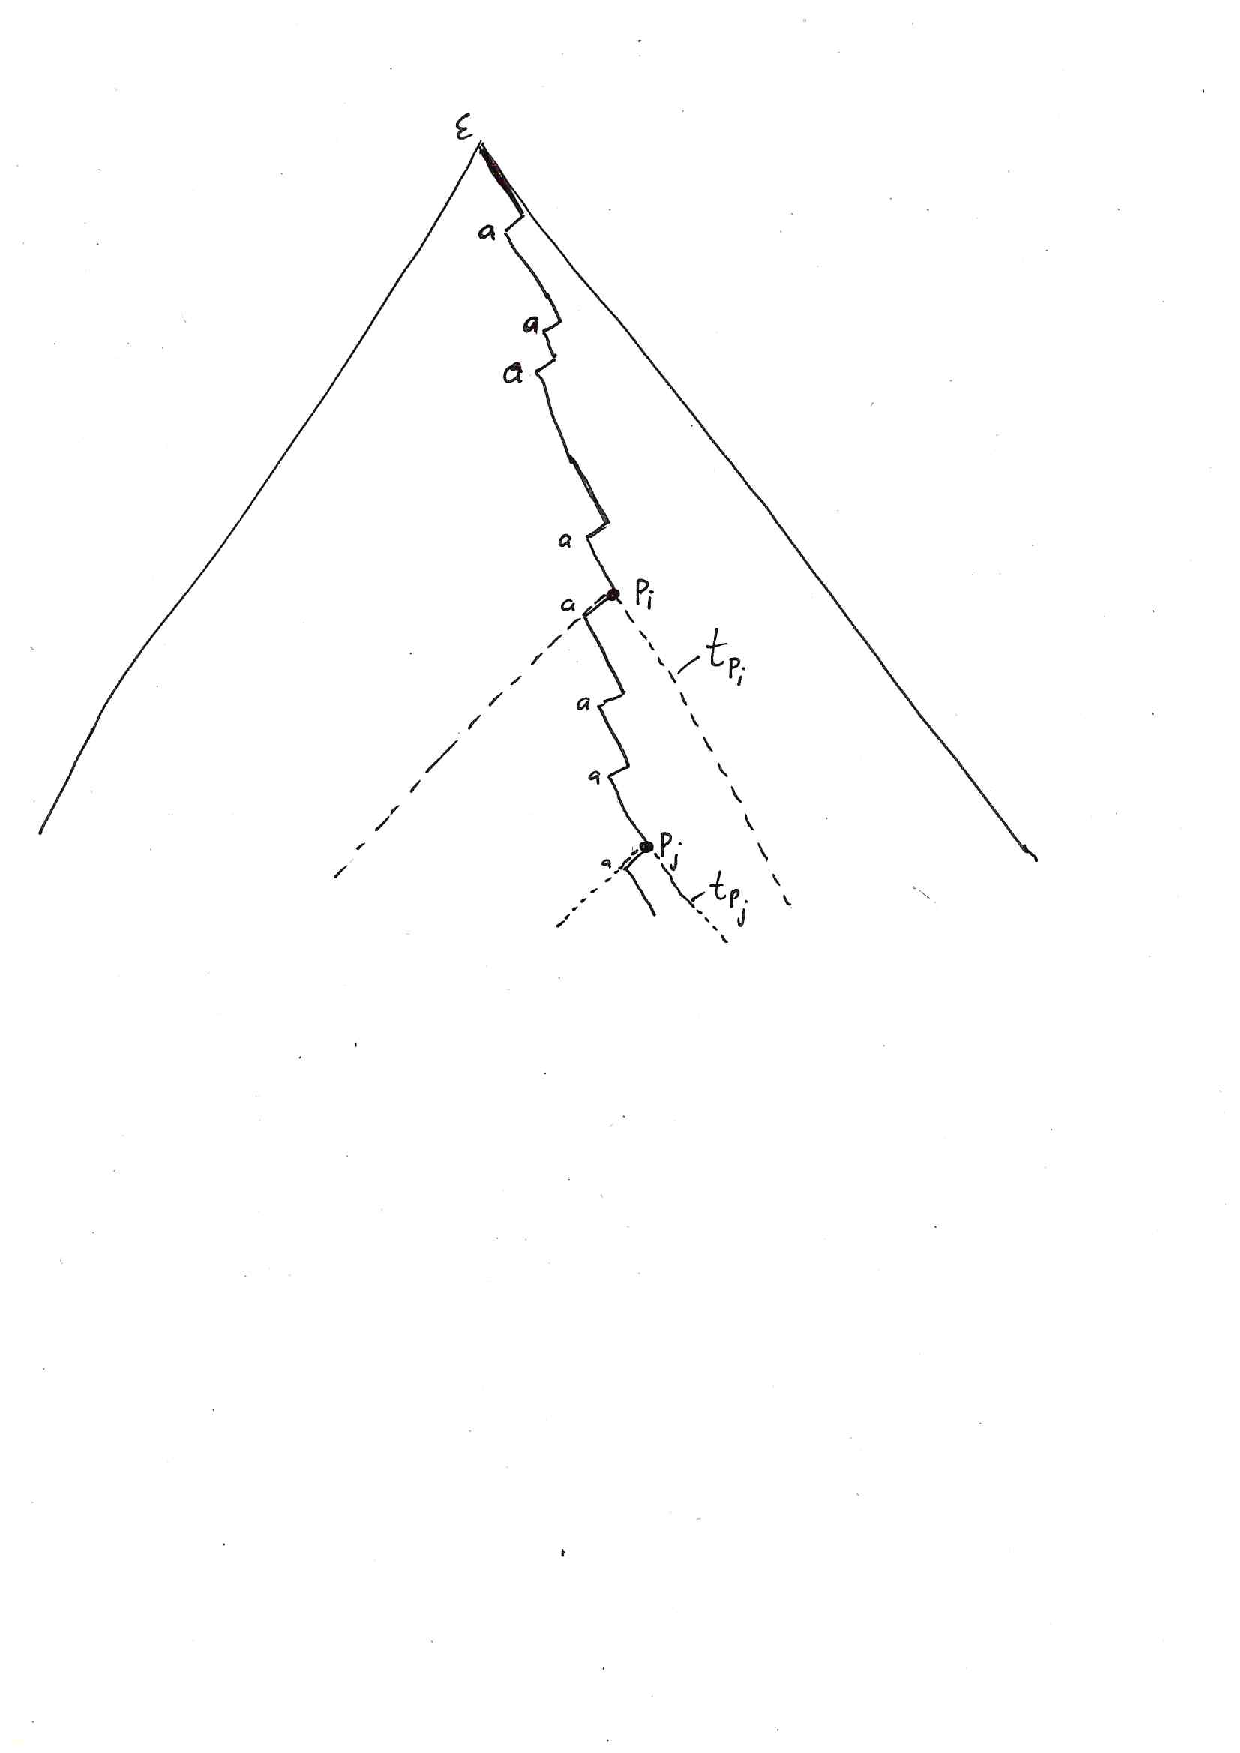
\includegraphics[width=.7\linewidth,trim=10 390 100 50,clip]{img/t4_6_skizze.pdf}
\end{center}
%
Nun gibt es in $t$ auf dem Pfad von der Wurzel zur Position $p_i$ genau $i < n$
"`Linksschritte"', also nach Definition von $t$ genau $i$ Positionen $p$ mit $t(p) = a$.
Da $i < j$, gibt es auf dem Pfad von $p_i$ zu $p_j$ mindestens einen weiteren
"`Linksschritt"', also mindestens eine Position $p$ mit $t(p)=a$.
Da $r(p_i)=r(p_j) \in F$,
können wir in $t$ (und $r$) den Teilbaum $t_{p_j}$ ($r_{p_j}$)
durch $t_{p_i}$ ($r_{p_i}$) ersetzen%
\footnote{%
  Wie in Kapitel 2 bezeichnet $t_p$ den Teilbaum des Baums $t$,
  dessen Wurzel $p$ ist.
}
und erhalten wieder einen erfolgreichen Run:
%
\begin{center}
  $r[p_j \to r_{p_i}]$ ist ein erfolgreicher Run auf $t[p_j \to t_{p_i}]$.\qquad $(*)$
\end{center}
%
Aussage $(*)$ gilt, weil
(a)~wegen $r(p_i)=r(p_j)$ weiterhin die Übergangsrelation $\Delta$ respektiert wird und
(b)~weiterhin auf allen Pfaden ein akzepzierender Zustand unendlich oft besucht werden muss.

Dieses Ersetzen kann nun unendlich oft iteriert werden.
Der auf diese Weise aus $r$ resultierende Baum ist ein erfolgreicher Run von \Amc
auf dem aus $t$ resultierenden Baum.
Letzterer hat jedoch einen Pfad mit unendlich vielen $a$'s,
ist also gar nicht in $L$ enthalten; ein Widerspruch.
\qedhere

% ===================================================================
\section*{{\boldmath T5.6~ Beispiel für die Konstruktion "`NMBA $\Rightarrow$ NPBA"'}}

Seien $Q=\{1,2,3\}$ und $F=\{1,2\}$.
Wir betrachten den Run $r=12131211\dots$ von \Amc auf einem Pfad $\pi$,
bei dem ab der 5.\ Position nur noch Zustände aus $F$ vorkommen.
Ein zugehöriger Run $r'$ von $\Amc'$ auf demselben Pfad ist:
%
\begin{center}
  $\auf 231,1\zu$\,
  $\auf 312,1\zu$\,
  $\auf 321,2\zu$\,
  $\auf 213,1\zu$\,
  $\auf 231,2\zu$\,
  $\auf 312,1\zu$\,
  $\auf 321,2\zu$\,
  $\auf 312,3\zu$
\end{center}
An der ersten Position sind alle Paare $\auf q_1q_2q_3,\ell\zu$ möglich,
in denen $q_3 = q_0$ ist, denn es gibt noch keine "`Vergangenheit"',
in der Zustände aufgetreten sein können.
Das Paar $\auf 312,1\zu$ an der zweiten Position gibt durch seine zweite
Komponente $\ell=1$ an, dass Zustand 2 (Ende der ersten Komponente 312)
in der vorangehenden Permutation (231) an 1.\ Stelle aufgetreten ist.
Ab Position 6 haben die Paare $\auf q_1q_2q_3,\ell\zu$
an den Positionen $q_2,q_3$ immer die akzeptierenden Zustände $1,2$,
und ab Position 7 ist $\ell > |Q|-|F| = 1$.

\goodbreak
% ===================================================================
\section*{{\boldmath T5.7~ Beweis der Hilfsaussage für "`NMBA $\Rightarrow$ NPBA"'}}

\begin{description}
  \item[{\boldmath"`$\Rightarrow$"'}]
    Wegen $\textsf{Inf}(q_0q_1q_2\cdots)=S$ gibt es Zeitpunkte
    %
    \begin{enumerate}
      \item[(i)]
        $m_1$, ab dem nur noch Zustände aus $S$ vorkommen,
        d.\,h.\ $q_i \in S$ für alle $i \geq m_1$;
      \item[(ii)]
        $m_2 > m_1$ so, dass während der Zeitpunkte $m_1,m_1+1,\dots,m_2$
        \emph{jeder} Zustand aus $S$ mindestens einmal vorkommt.
    \end{enumerate}
    %
    Daraus folgt
    %
    \begin{enumerate}
      \item[(i$'$)]
        Für alle $i \geq m_1$ werden nur noch Zustände aus $S$ in die Endposition von
        $\textsf{perm}_i$ gerückt
      \item[(ii$'$)]
        Bis $m_2$ wurde \emph{jeder} Zustand aus $S$ mindestens einmal in die 
        Endposition von
        $\textsf{perm}_i$ gerückt.
    \end{enumerate}
    %
    Wegen (ii$'$) müssen die letzten $k$ Positionen von $\textsf{perm}_{m_2}$
    genau die $k$ Zustände aus $S$ enthalten
    (und die ersten $n-k$ Positionen die Zustände aus $Q\setminus S$).
    In zukünftigen Zuständen $s_i$ mit $i > m_2$ wird
    nie ein Zustand aus $Q\setminus S$ in die Endposition von $\textsf{perm}_i$ gerückt;
    also ist $\ell_i  > n-k$ (was Teil~(1) der Hilfsaussage beweist),
    und die letzten $k$ Positionen in $\textsf{perm}_i$ sind aus $S$
    (was Teil~(2)\,(b) beweist).
    
    Um Teil~(2)\,(a) zu zeigen, nehmen wir an, es sei $\ell_i = n-k+1$
    für nur endlich viele $i$.
    Dann müsste es aber einen Zustand aus $S$ geben, der nur endlich oft besucht wird
    und deshalb dauerhaft in Position $n-k+1$ von $\textsf{perm}_i$ landet.
    Dies ist aber ein Widerspruch zu $\textsf{Inf}(q_0q_1q_2\cdots)=S$.
  \item[{\boldmath"`$\Leftarrow$"'}]
    Kann mit einer ähnlichen Argumentation,
    die die Konstruktion analysiert,
    bewiesen werden.
    \qedhere
\end{description}

\pagebreak
% ===================================================================
\section*{{\boldmath T5.8~ Beweis der Korrektheit, "`NMBA $\Rightarrow$ NPBA"'}}

Es bleibt zu zeigen: $L_\omega(\Amc) = L_\omega(\Amc')$.
%
\begin{description}
  \item[{\boldmath"`$\subseteq$"'}]
    Sei $t \in L_\omega(\Amc)$.
    Dann gibt es einen erfolgreichen Run $r$ von $\Amc$ auf $t$,
    d.\,h.\ $\textsf{Inf}(r,\pi) = F$ für alle Pfade $\pi$ von $t$.
    
    Sei $s_0 = \auf t_1\cdots t_{n-1}q_0,1\zu \in I'$,
    und sei $s$ der gemäß $\Delta'$ eindeutig bestimmte Run von $\Amc'$ auf $t$,
    der folgende Eigenschaften erfüllt.
    %
    \begin{enumerate}
      \item[(i)]
        $s(\varepsilon) = s_0$
      \item[(ii)]
        Für alle $p \in \{0,1\}^*$ hat $s(p)$ die Form $\auf \textsf{perm}_p,\ell_p\zu$,
        wobei $\textsf{perm}_p$ auf $r(p)$ endet.
    \end{enumerate}
    %
    Wir müssen noch zeigen, dass $s$ erfolgreich ist.
    Dazu betrachten wir einen beliebigen Pfad $\pi$
    und die zugehörige Zustandsfolge $s_0s_1s_2\cdots$ von $s$
    mit $s_i = \auf \textsf{perm}_i,\ell_i\zu$.
    Da $r$ erfolgreich ist, gilt $\textsf{Inf}(r,\pi) = F$.
    Wegen der Hilfsaussage folgt daraus:
    %
    \begin{enumerate}
      \item[(1)]
        Für endlich viele $i$ ist $\ell_i \leq n - |F|$.
      \item[(2)]
        Für unendlich viele $i$ gilt:
        %
        \begin{enumerate}
          \item[(a)]
            $\ell_i = n - |F| + 1$
          \item[(b)]
            Die Menge der Zustände an den Positionen $n - |F| + 1,\dots,n$ in $\textsf{perm}_i$ ist $F$.
        \end{enumerate}
    \end{enumerate}
    %
    Wegen (2) muss $\textsf{Inf}(s,\pi)$ einen Zustand der Form 
    $\auf q_1\cdots q_n, n-|F|+1\zu$ mit $\{q_{n-|F|+1},\dots,q_n\} = F$ enthalten,
    aber wegen (1) \emph{keinen} Zustand der Form
    $\auf q_1\cdots q_n,\ell\zu$ für $\ell \leq n-|F|$.
    Damit erfüllt der Pfad $\pi$ in $s$ die Akzeptanzbedingung von $\Amc'$;
    also ist $t \in L_\omega(\Amc')$.
    \par\medskip
  \item[{\boldmath"`$\supseteq$"'}]
    Sei $t \in L_\omega(\Amc')$.
    Dann gibt es einen erfolgreichen Run $s$ von $\Amc'$ auf $t$.
    Sei $s(p) = \auf \textsf{perm}_p,\ell_p\zu$.
    Wir konstruieren einen Run $r$ von $\Amc$ auf $t$, indem
    wir $r(p)$ auf das letzte Element von $\textsf{perm}_p$ setzen,
    für alle $p \in \{0,1\}^*$.
    Nach Definition von $I'$ und $\Delta'$ ist dann nämlich
    %
    \begin{itemize}
      \item
        $r(\varepsilon) \in I'$\quad und
      \item
        $\Big(r(p),t(p),r(p0),r(p1)\Big) \in \Delta$ für alle $p \in \{0,1\}^*$,
    \end{itemize}
    %
    also ist $r$ tatsächlich ein Run von $\Amc$ auf $t$.
%    
    Es bleibt zu zeigen,
    dass $r$ erfolgreich ist.
    Dazu betrachten wir einen beliebigen Pfad $\pi$.
    Da $s$ erfolgreich ist und wegen der Akzeptanzbedingung von $\Amc'$
    gibt es einen Zustand $\auf q_1\cdots q_n,\ell\zu$ mit $\{q_\ell,\dots,q_n\} = F$,
    so dass
    %
    \begin{enumerate}
      \item[(i)]
        $\auf q_1\cdots q_n,\ell\zu$ unendlich oft in $s$ auftritt,\quad aber
      \item[(ii)]
        \emph{kein} $\auf q_1'\cdots q_n',\ell'\zu$ mit $\{q_1',\dots,q_n'\} \neq F$ und $\ell' < \ell$ unendlich oft auftritt.
    \end{enumerate}
    %
    Die Eigenschaften (i) und (ii) entsprechen aber genau den Teilen
    (2) bzw.\ (1) aus der Hilfsaussage,
    also gilt $\textsf{Inf}(r,\pi) = \{q_\ell,\dots,q_n\}=F$.
    Damit ist $t \in L_\omega(\Amc)$.
    \qedhere
\end{description}

% ===================================================================
\section*{{\boldmath T5.9~ Beispiel eines Spielverlaufs für \Game{A}{t}}}

Wir betrachten den NPBA von Folie~5.41,
d.\,h.\
%
\begin{align*}
  \Amc   & = (\{A,B\},~\{a,b\},~\Delta,~\{A\},~c) \qquad \text{mit} \\
  \Delta & = \{(A,a,A,A),~(B,a,A,A),~(A,b,B,B),~(B,b,B,B)\} \qquad\text{und} \\
  c      & ~:~~ A \mapsto 1,~ B \mapsto 2.
\end{align*}
%
Zur Erinnerung: $L_\omega(\Amc) = \{t \mid \text{jeder Pfad in $t$ hat endlich viele $a$'s}\}$.

Wir betrachten folgenden Eingabebaum $t$.
%
\newcommand{\Baum}{%
  \begin{scope}[
    every node/.style={circle,draw=black,thin,fill=black!5,inner sep=1mm,minimum size=6mm},
    level 1/.style = {sibling distance = 64mm, level distance =  6mm},
    level 2/.style = {sibling distance = 30mm, level distance =  9mm},
    level 3/.style = {sibling distance = 13mm, level distance =  11mm},
    level 4/.style = {sibling distance = 8mm, level distance = 11mm},
    edge from parent/.style = {draw=black, thin, -}%
  ]
    \node (eps) {$a$}
    child {
      node (0) {$b$}
      child {
        node (00) {$b$}
        child {
          node (000) {$b$}
        }
        child {
          node (001) {$b$}
        }
      }
      child {
        node (01) {$a$}
        child {
          node (010) {$b$}
          child {
            node (0100) {$b$}
          }
          child {
            node (0101) {$a$}
          }
        }
        child {
          node (011) {$b$}
        }
      }
    }
    child {
      node (1) {$b$}
      child {
        node (10) {$b$}
      }
      child {
        node (11) {$b$}
      }
    }
    ;
  \end{scope}
    
  \foreach \x in {000,001,0100,0101,011,10,11}
    \node [draw=none,fill=none,below=-1mm of \x] {$\vdots$};
}
\newcommand{\labeleps}{%
  \node [draw=none,fill=none,above right=-2mm and 0mm of eps] {$(\varepsilon,A)$};
}
\newcommand{\labelone}{%
  \node [draw=none,fill=none,above right=-5mm and .8mm of 1] {$(1,A)$};
  \path[-] (eps) edge[draw=black,line width=2mm,draw opacity=.4] (1);
}
\newcommand{\labelonezero}{%
  \node [draw=none,fill=none,left=0mm of 10] {$(10,B)$};
  \path[-] (1) edge[draw=black,line width=2mm,draw opacity=.4] (10);
}
%
\begin{center}
  \begin{tikzpicture}[node distance=20mm,>=Latex]
    \Baum
    \path[-,draw=black,line width=2mm,draw opacity=.4] 
      (eps) edge (0)
      (0)   edge (01)
      (01)  edge (010)
      (010) edge (0101)
      ;
  \end{tikzpicture}
\end{center}
%
In $t$ ist der hervorgehobene Pfad $(01)^\omega$ abwechselnd mit $a$'s und $b$'s beschriftet;
an allen anderen Positionen stehen $b$'s. Folglich ist $t \notin L_\omega(\Amc)$.

Wir betrachten nun die ersten zwei Runden eines Spielverlaufs
im Spiel $\Game{A}{t}$\,.
In der anfänglichen Spielposition ist nur die Wurzel mit dem Anfangszustand $A$ markiert;
also ist der bisherige Spielverlauf die Folge, die nur aus dem Paar
$(\varepsilon,A)$ besteht. Zur Veranschaulichung wird der Spielverlauf
im Folgenden an den von \PF gewählten Pfad im Baum geschrieben, also
zu Beginn so:
%
%\par\vspace*{-2\baselineskip}
\begin{center}
  \begin{tikzpicture}[node distance=20mm,>=Latex]
    \Baum    
    \labeleps
  \end{tikzpicture}
\end{center}
%
In der ersten Runde wählt \AUT die einzige zum Zustand $A$ und Zeichen $a$
passende Transition $(A,a,A,A)$,
und \PF antwortet darauf mit der Wahl des rechten Kindknotens.
Dadurch ist nun das rechte Kind der Wurzel mit $A$ markiert:
%
%\par\vspace*{-\baselineskip}
\begin{center}
  \begin{tikzpicture}[node distance=20mm,>=Latex]
    \Baum    
    \labeleps
    \labelone
  \end{tikzpicture}
\end{center}
%
In der zweiten Runde wählt \AUT die einzige zum Zustand $A$ und Zeichen $b$
passende Transition $(A,b,B,B)$,
und \PF antwortet darauf mit der Wahl des linken Kindknotens.
Dadurch ist nun das linke Kind der zuletzt betrachteten Position mit $B$ markiert:
%
%\par\vspace*{-\baselineskip}
\begin{center}
  \begin{tikzpicture}[node distance=20mm,>=Latex]
    \Baum    
    \labeleps
    \labelone
    \labelonezero
  \end{tikzpicture}
\end{center}
%
%\par\vspace*{-\baselineskip}
Es ist klar, dass in diesem Spiel \AUT gewinnt, weil in den folgenden Runden nur noch
$b$'s gelesen und damit nur noch der Zustand $B$ eingenommen wird.
Damit kommt $A$ endlich oft und $B$ unendlich oft auf dem gespielten Pfad vor,
und die durch $c$ gegebene Akzeptanzbedingung ist erfüllt. Folglich gewinnt \AUT
diesen Spielverlauf.

Würde \PF in Runde 1 den linken und danach immer im Wechsel den linken und rechten
Nachfolger der aktuellen Position wählen, dann wird der "`defekte"' Pfad $(10)^\omega$
sichtbar gemacht, auf welchem die Akzeptanzbedingung \emph{nicht} erfüllt ist.
In diesem Spielverlauf gewinnt \PF.

Man beachte bei beiden Spielverläufen: da der gegebene NPBA deterministisch ist,
hat \AUT in jeder Runde nur eine mögliche Transition zur Auswahl.
Im Allgemeinen hat \AUT natürlich mehrere Wahlmöglichkeiten.

\goodbreak
% ===================================================================
\section*{T5.10~ Beispiel für Gewinnstrategie}

Wir betrachten den NPBA \Amc und die Eingabe $t$ aus dem letzten Beispiel.
Eine Gewinnstrategie für \PF ab Spielposition $v$ ist folgende:
%
\begin{center}
  \parbox{.8\linewidth}{%
    In Spielposition $v'$, die durch die Zugfolge $v\cdots v'$ bestimmt ist, \\
    wobei $v'=\big(q,t(p),q',q''\big)$ mit $q,q',q'' \in \{A,B\}$,
    \par\smallskip
    wähle das linke Kind, wenn $t(p)=a$ und das rechte Kind, wenn $t(p)=b$. %\\
%    (wegen $\Sigma=\{a,b\}$ muss immer einer dieser beiden Fälle eintreten).%
  }
\end{center}
%
Diese Strategie stellt eine Funktion $f$ dar, die jeder Zugfolge $v\cdots v'$
einen eindeutig bestimmten Zug von \PF (linkes/rechtes Kind) zuweist.
Sie ist eine Gewinnstrategie, denn sie stellt sicher, dass unabhängig davon, wie \AUT spielt (hier hat \AUT sowieso keine Wahl),
auf dem gesamten gespielten Pfad Zustand $A$ unendlich oft auftritt;
also ist die Akzeptanzbedingung von \Amc verletzt.

\goodbreak
In dieser Gewinnstrategie für den sehr einfachen Automaten $\Amc$ hängt
$f(v\cdots v')$ nur von $v'$ ab und nicht von den vorhergehenden Spielpositionen
in $v\cdots v'$. Die Strategie ist also \emph{gedächtnislos},
was intuitiv so viel bedeutet wie: "`der bisherige Spielverlauf kann
ignoriert/vergessen werden"'.
Satz 5.18 und Folgerung 5.19 zeigen, dass dies nicht an der
Einfachheit von $\Amc$ liegt.

\goodbreak
%% ===================================================================
%\section*{T5.11~ Beweis der Rückrichtung von Lemma~5.17}
%
%\textsfbf{Behauptung.}~
%\AUT hat Gewinnstrategie in $\Game{A}{t}$ ab Position $(\varepsilon,q_I)$ ~$\Rightarrow$~ $t \in L_\omega(\Amc)$
%
%\par\medskip
%\textsfbf{Beweis.}~
%Habe \AUT eine Gewinnstrategie in $\Game{A}{t}$ ab Position $(\varepsilon,q_I)$.
%Wir konstruieren einen erfolgreichen Run $r$ von \Amc auf $t$
%induktiv über die Ebenen von $t$:
%%
%\begin{itemize}
%  \item
%    $r(\varepsilon) = q_I$
%  \item
%    Wenn $r(p)$ definiert ist,
%    dann betrachte die Transition $\big(r(p),t(p),q_0,q_1\big)$,
%    die durch die Gewinnstrategie der Position $\big(p,r(p)\big)$
%    zugewiesen wird.
%    Setze $r(p0) = q_0$ und $r(p1) = q_1$.
%\end{itemize}
%%
%Nach Definition der Spielzüge von \AUT ist $r$ ein Run von $\Amc$ auf $t$.
%Außerdem ist $r$ erfolgreich,
%denn sonst gäbe es einen Pfad in $t$, auf dem die Akzeptanzbedingung von $\Amc$
%nicht erfüllt wäre. Dann könnte aber \AUT verlieren, indem \PF diesen Pfad wählt,
%was ein Widerspruch zur Annahme wäre, dass \AUT eine Gewinnstrategie hat.
%\qedhere

%\pagebreak
% ===================================================================
\section*{T5.11~ Beweis von Lemma~5.17}

\textsfbf{Lemma 5.17.}~
Seien $\Amc = (Q,\Sigma,\Delta,\{q_I\},c)$ ein NPBA und $t$ ein $\Sigma$-Baum.
Dann gilt:
$t \in L_\omega(\Amc)$ ~\textsfbf{gdw.}~ \AUT hat Gewinnstrategie in $\Game{A}{t}$ ab Position $(\varepsilon,q_I)$

\par\medskip
\textsfbf{Beweis.}~
Wir wandeln erfolgreiche Runs direkt in Gewinnstrategien
und umgekehrt.
%
\begin{description}
  \item[{\boldmath "`$\Rightarrow$"'}] 
    Gelte $t \in L_\omega(\Amc)$ und sei $r$ erfolgreicher Run von $\Amc$ auf $t$.
    Die Gewinnstrategie für \AUT lässt sich leicht wie folgt aus $r$ konstruieren.
    %
    \begin{itemize}
      \item
        In Startposition $(\varepsilon,q_I)$ wähle
        $(r(\varepsilon),t(\varepsilon),r(0),r(1))$.
      \item
        In allen anderen Spielpositionen $(p,q)$ wähle
        $(q,t(p),r(p0),r(p1))$.
    \end{itemize}
    %
    Wenn \AUT diese Strategie befolgt,
    dann entspricht die im Spiel erzeugte Zustandsmenge
    einem Pfad in $r$.
    Da $r$ erfolgreich ist, gewinnt \AUT nach Def.\ von $G_{\Amc,t}$\,.
    \parI
  \item[{\boldmath "`$\Leftarrow$"'}] 
    Habe \AUT eine Gewinnstrategie in $\Game{A}{t}$ ab Position $(\varepsilon,q_I)$.
    Wir konstruieren einen erfolgreichen Run $r$ von \Amc auf $t$
    induktiv über die Ebenen von $t$:
    %
    \begin{itemize}
      \item
        $r(\varepsilon) = q_I$
      \item
        Wenn $r(p)$ definiert ist,
        dann betrachte die Transition $\big(r(p),t(p),q_0,q_1\big)$,
        die durch die Gewinnstrategie der Spielposition $\big(p,r(p)\big)$
        zugewiesen wird.
        Setze $r(p0) = q_0$ und $r(p1) = q_1$.
    \end{itemize}
    %
    Nach Definition der Spielzüge von \AUT ist $r$ ein Run von $\Amc$ auf $t$.
    Außerdem ist $r$ erfolgreich,
    denn sonst gäbe es einen Pfad in $t$, auf dem die Akzeptanzbedingung von $\Amc$
    nicht erfüllt wäre. Dann könnte aber \AUT verlieren, indem \PF diesen Pfad wählt
    -- Widerspruch zur Annahme, dass \AUT eine Gewinnstrategie hat.
    \qedhere
\end{description}

% ===================================================================
\section*{T5.12~ {\boldmath Beispiel für einen Gewinnbaum}}

Wir betrachten wieder den NPBA \Amc und die Eingabe $t$ aus T5.9 und T5.10
und formulieren die genannte gedächtnislose Gewinnstrategie von \PF
als Baum von Funktionen.
So ist beispielsweise $f_\varepsilon$ gegeben durch:
%
\begin{align*}
f_\varepsilon : {} & (A,a,A,A) \mapsto 0 \\
                   & (B,a,A,A) \mapsto 0 \\
                   & (A,b,B,B) \mapsto 0 \\
                   & (B,b,B,B) \mapsto 0
\end{align*}
%
Dabei ist der Funktionswert nur in der ersten Zeile relevant,
denn in Spielposition $(\varepsilon,A)$ kann \AUT nur die erste Transition spielen.
In den übrigen drei Zeilen kann also durchaus ein anderer Wert stehen,
d.\,h.\ es gibt mehrere \PF-Gewinnbäume für $\Amc,t$.

Analog dazu ist $f_0$ gegeben durch:
%
\begin{align*}
f_0 : {} & (A,a,A,A) \mapsto 0 \\
         & (B,a,A,A) \mapsto 0 \\
         & (A,b,B,B) \mapsto 1 \\
         & (B,b,B,B) \mapsto 0
\end{align*}
%
Auch hier ist wieder nur eine Zeile relevant, nämlich die dritte,
denn in Spielposition $(0,A)$ kann \AUT nur die dritte Transition spielen.

Da $\Delta$ aus 4 Transitionen besteht, können alle Funktionen
als 4-Tupel geschrieben werden, also z.\,B.\ $f_\varepsilon = 0000$
und $f_0 = 0010$.
Insgesamt gibt es in $F$ (Menge aller Funktionen $f : \Delta \to \{0,1\}$)
somit $2^4 = 16$ Funktionen, die wir der Einfachheit halber durchnummerieren
als $F = \{f^0,\dots,f^{15}\} = \{0000,0001,\dots,1111\}$.
Damit ist $f_\varepsilon = f^0$ und $f_0 = f^2$.

Ein möglicher \PF-Gewinnbaum für $\Amc,t$ beinhaltet somit nur die Funktionen
$f^0$ und $f^2$:
%
\begin{center}
  \begin{tikzpicture}[
    node distance=20mm,>=Latex,
    every node/.style={circle,draw=black,thin,fill=black!5,inner sep=1mm,minimum size=6mm},
    level 1/.style = {sibling distance = 64mm, level distance =  6mm},
    level 2/.style = {sibling distance = 30mm, level distance =  9mm},
    level 3/.style = {sibling distance = 13mm, level distance =  11mm},
    level 4/.style = {sibling distance = 8mm, level distance = 11mm},
    edge from parent/.style = {draw=black, thin, -}%
  ]
    \node (eps) {$f^0$}
    child {
      node (0) {$f^2$}
      child {
        node (00) {$f^0$}
      }
      child {
        node (01) {$f^0$}
      }
    }
    child {
      node (1) {$f^0$}
      child {
        node (10) {$f^0$}
      }
      child {
        node (11) {$f^0$}
      }
    }
    ;

  \foreach \x in {00,01,10,11}
    \node [draw=none,fill=none,below=-1mm of \x] {$\vdots$};

    \path[-,draw=black,line width=2mm,draw opacity=.4] 
      (eps) edge (0)
      (0)   edge (01)
      ;
  \end{tikzpicture}
\end{center}
%
Wie oben bereits angedeutet, gibt es mehrere \PF-Gewinnbäume für $\Amc,t$:
es ist nur wichtig, dass auf dem hervorgehobenen Pfad abwechselnd
$f^0$ und $f^2$ auftreten; in allen übrigen Positionen ist die Wahl der Funktion
irrelevant für das Gewinnen von \PF, denn die Akzeptanzbedingung ist auf allen
übrigen Pfaden wegen der $b$'s sowieso erfüllt.



% ===================================================================
\section*{T5.13~ {\boldmath Beispiel für die Sprache \Lst}}

Ab jetzt bezeichnen wir Pfade im Baum als Wörter $\pi \in \{0,1\}^*$;
beispielsweise steht $\pi = 0110\cdots$
für den Pfad $\{\varepsilon,0,01,011,\dots\}$.

Sei $t$ ein beliebiger Baum, $s$ ein Strategiebaum (der nach Definition
für jede Position $p \in \{0,1\}^*$ eine Funktion $f_p : \Delta \to \{0,1\}$ enthält)
und $\pi = 0110\cdots$.
Dann wird durch $\pi$ folgendes $\omega$-Wort $\alpha \in \Lst$ bestimmt:
%
\begin{center}
  $\alpha ~=~ {}$
  \newcommand{\Tripel}[3]{
    ~\begin{tabular}{@{}c@{}}#1\\[3pt]#2\\[3pt]#3\end{tabular}\,%
  }%
  \begin{tikzpicture}[
    baseline=-2pt,
    every node/.style={rectangle,rounded corners,draw=black,thin,inner sep=1mm}
  ]
    \node                 (0) {\Tripel{$f_\varepsilon$}{$t(\varepsilon)$}{0}};
    \node[right=3mm of 0] (1) {\Tripel{$f_0$}{$t(0)$}{1}};
    \node[right=3mm of 1] (2) {\Tripel{$f_{01}$}{$t(01)$}{1}};
    \node[right=3mm of 2] (3) {\Tripel{$f_{011}$}{$t(011)$}{0}};
    \node[right=3mm of 3] (4) {\Tripel{$f_{0110}$}{$t(0110)$}{0}};
    \node[right=3mm of 4,draw=none] (5) {$\cdots$};
  \end{tikzpicture}
\end{center}
%
Dabei bezeichnet jede Box ein Symbol von $\alpha$, also gemäß Folie~5.55 ein Tripel,
und jede erste Komponente $f_p$ eines Tripels
steht wiederum für dasjenige $|\Delta|$-Tupel von Nullen und Einsen,
welches $f_p$ repräsentiert.
Das erste Zeichen von $\alpha$ ist also $\big\auf f_\varepsilon,t(\varepsilon),0\big\zu$.

Mit anderen Worten: die Folge $f_\varepsilon,f_0,f_{01},\dots$
aller ersten Komponenten der Zeichen von $\alpha$ gibt den Inhalt von $s$
auf dem Pfad $\pi$ wieder und die Folge aller zweiten Komponenten 
den Inhalt von $t$ auf $\pi$. Die Folge der dritten Komponenten
ist $\pi$ selbst.

\goodbreak
% ===================================================================
\section*{T5.14~ Beweis von Lemma~5.22}

\textsfbf{Lemma~5.22.}~
$s$ ist ein \PF-Gewinnbaum für $\Amc,t$
~gdw.~
$\Lst \cap L_\omega(\Amc') = \emptyset$

\par\medskip
\textsfbf{Beweis.}~
\begin{description}
  \item[{\boldmath"`$\Rightarrow$"'}]
%    Sei $s$ ein \PF-Gewinnbaum für $\Amc,t$.
%    Wir nehmen an, $\Lst \cap L_\omega(\Amc') \neq \emptyset$.
    Wir beweisen die Kontraposition.
    Gelte $\Lst \cap L_\omega(\Amc') \neq \emptyset$.
    Dann gibt es einen Pfad $\pi$,
    so dass das $\Sigma'$-Wort
    \[
      \alpha = 
      \big\auf s(\varepsilon),t(\varepsilon),\pi_1\big\zu~
      \big\auf s(\pi_1),t(\pi_1),\pi_2\big\zu~
      \big\auf s(\pi_1\pi_2),t(\pi_1\pi_2),\pi_3\big\zu~
      \cdots
    \]
    von $\Amc'$ akzeptiert wird.
    Sei $r=q_0q_1q_2\cdots$ ein erfolgreicher Run von $\Amc'$ auf $\alpha$.
    Dann gibt es für jede Position $j \geq 0$ in $\alpha$ eine Transition
    \[
      \Big(q_j,~\big\auf s(\pi_1\cdots\pi_j),t(\pi_1\cdots\pi_j),\pi_{j+1}\big\zu,~q_{j+1}\Big) ~\in~ \Delta'.
    \]
    Nach Konstruktion von $\Delta'$ gibt es dann in $\Amc$ eine entsprechende Transition
    \[
      \delta_j = \Big(q_j,~t(\pi_1\cdots\pi_j),~q_0',~q_1'\Big) ~\in~ \Delta
    \]
    mit $s(\pi_1\cdots\pi_j)(\delta_j) = \pi_{i+1}$,
    wobei $s(\pi_1\cdots\pi_j)$ die Funktion $f_{\pi_1\cdots\pi_j} \in F$ ist.
    
    Wir betrachten nun denjenigen Spielverlauf von $\Game{A}{t}$,
    in dem \AUT in Spielposition $\pi_1\cdots\pi_j$ jeweils $\delta_j$ wählt
    und daraufhin \PF mit $s(\pi_1\cdots\pi_j) = \pi_{j+1}$ antwortet.
    Die während dieses Spiels erzeugte Zustandsfolge ist genau der Run $r$,
    also gewinnt \AUT (denn $\Amc'$ hat nach Konstruktion dieselbe Akzeptanzkomponente $c$
    wie $\Amc$).
    In diesem Spielverlauf verliert also \PF, obwohl sie nach Strategie $s$ gespielt hat.
    Folglich ist $s$ kein \PF-Gewinnbaum für $\Amc,t$.
    \par\medskip
  \item[{\boldmath"`$\Leftarrow$"'}]
    Gelte $\Lst \cap L_\omega(\Amc') = \emptyset$.
    Wir betrachten einen beliebigen Spielverlauf von $\Game{A}{t}$ ab
    $(\varepsilon,q_I)$, bei dem
    \PF nach Strategie $s$ spielt, d.\,h.\
    für alle $j \geq 0$
    %
    \begin{itemize}
      \item
        wählt \AUT in Spielposition $(\pi_1\cdots\pi_j,\,q_j)$
        eine beliebige Transition 
        \[
          \delta_j = \Big(q_j,~ t(\pi_1\cdots \pi_j),~ q_{j0}, q_{j1}\Big) ~\in~ \Delta
          \qquad\text{und}
        \]
      \item
        \PF antwortet mit $q_{j+1}$ gemäß $s$:
        \[
          q_{j+1} = 
          \begin{cases}
            q_{j0} & \text{falls~} s(\pi_1\cdots\pi_j)(\delta_j) = 0 \\
            q_{j1} & \text{sonst}
          \end{cases}
        \]
    \end{itemize}
    %
    Wir betrachten nun die Folge $r'=q_0q_1q_2\cdots$ der während des Spielverlaufs
    besuchten Zustände.
    Nach Konstruktion von $\Delta'$ ist $r'$ ein Run von $\Amc'$ auf dem
    zugehörigen $\omega$-Wort
    \[
      \alpha = 
      \big\auf s(\varepsilon),t(\varepsilon),\pi_1\big\zu~
      \big\auf s(\pi_1),t(\pi_1),\pi_2\big\zu~
      \big\auf s(\pi_1\pi_2),t(\pi_1\pi_2),\pi_3\big\zu~
      \cdots
      \in \Lst.
    \]
    Da $\Lst \cap L_\omega(\Amc') = \emptyset$, ist $r'$ nicht erfolgreich.
    Der Run $r'$ entspricht außerdem einem Pfad eines Runs des ursprünglichen $\Amc$ auf $t$,
    nämlich desjenigen Runs $r$, der durch die Entscheidungen von \AUT bestimmt wird.
    Deshalb kann $r$ nicht erfolgreich sein.
    Wir haben also für eine \emph{beliebige} Zugfolge von \AUT gezeigt, 
    dass der zugehörige Run von \Amc auf $t$ nicht erfolgreich sein kann.
    Somit muss $s$ eine Gewinnstrategie für \PF kodieren,
    ist also ein \PF-Gewinnbaum für $\Amc,t$.
    \qedhere
\end{description}

\goodbreak
% ===================================================================
\section*{T5.15~ Beweis von Lemma~5.23}

\textsfbf{Lemma~5.23.}~
$t \in L_\omega(\Bmc)$
~gdw.~
es gibt $F$-Baum $s$ mit $\Lst \subseteq L_\omega(\Amc'')$

\par\medskip
\textsfbf{Beweis.}~
\begin{description}
  \item[{\boldmath"`$\Rightarrow$"'}]
    Sei $t \in L_\omega(\Bmc)$ und $r$ ein erfolgreicher Run von \Bmc auf $t$,
    d.\,h.
    %
    \begin{itemize}
      \item[(i)] 
        für jede Baumposition $p \in \{0,1\}^*$ gibt es in $\Delta^{\textsf{neu}}$
        einen entsprechenden Übergang $\big(r(p),t(p),r(p0),r(p1)\big)$ \qquad und
      \item[(ii)]
        $r$ erfüllt auf jedem Pfad die Akzeptanzbedingung
        $c''$ von $\Amc''$ (diese hat ja $\Bmc$ von $\Amc''$ übernommen).
    \end{itemize}
    %
    Aus (i) und der Konstruktion von $\Delta^{\textsf{neu}}$ folgt,
    dass es für jedes $p$ eine Funktion $f_p \in F$ gibt mit
    %
    \begin{align*}
      \Big(r(p),~ \big\auf f_p,t(p),0\zu,~ r(p0)\Big) & \in \Delta''\qquad\text{und} \tag{iii}\\
      \Big(r(p),~ \big\auf f_p,t(p),1\zu,~ r(p1)\Big) & \in \Delta'' \tag{iv}.
    \end{align*}
    %
    Sei nun $s$ der durch diese $f_p$ bestimmte $F$-Baum,
    d.\,h.\ $s(p) = f_p$.
    
    Wir betrachten einen beliebigen Pfad $\pi = \pi_1\pi_2\pi_3\cdots$
    und das zugehörige $\omega$-Wort
    \[
      \alpha_\pi = 
      \big\auf s(\varepsilon),t(\varepsilon),\pi_1\big\zu~
      \big\auf s(\pi_1),t(\pi_1),\pi_2\big\zu~
      \big\auf s(\pi_1\pi_2),t(\pi_1\pi_2),\pi_3\big\zu~
      \cdots
      \tag{$*$}
    \]
    aus \Lst.
    Es bleibt zu zeigen, dass $\alpha_\pi \in L_\omega(\Amc'')$ ist.
    Dies folgt, weil (i), (iii) und (iv) "`bezeugen"', dass $r$
    ein erfolgreicher Run von $\Amc''$ auf $\alpha_\pi$ ist.
    \par\medskip
  \item[{\boldmath"`$\Leftarrow$"'}]
    Seien $t,s$ so, dass $\Lst \subseteq L_\omega(\Amc'')$.
    Um zu zeigen, dass $t \in L_\omega(\Bmc)$, konstruieren wir einen
    erfolgreichen Run aus allen Pfaden, die $\Amc''$ akzeptiert.
    Dabei benutzen wir, dass $\Amc''$ deterministisch ist.
    
    Wegen $\Lst \subseteq L_\omega(\Amc'')$ gibt es für jeden Pfad $\pi$
    einen erfolgreichen Run von $\Amc''$ auf dem Wort $\alpha_\pi$,
    das gemäß $(*)$ definiert ist.
    Da $\Amc''$ deterministisch ist, sind seine Runs auf Wörten aus \Lst
    eindeutig bestimmt.
    Insbesondere gilt: wenn zwei Pfade $\pi,\pi'$ dasselbe Präfix
    $\pi_1\cdots\pi_k=\pi_1'\cdots\pi_k'$ haben,
    dann weisen die beiden eindeutig bestimmten Runs von $\Amc''$
    den ersten $k$ Positionen der zugehörigen Wörter aus \Lst
    dieselben Zustände zu.
    Das heißt, dass es für jede Position $p$ einen \emph{eindeutig bestimmten}
    Zustand $q$ gibt, so dass für alle Pfade $\pi$ mit $p=\pi_1\cdots\pi_k$
    der Run von $\Amc''$ "`auf $\pi$"' der Position $k$ den Zustand $q$ zuweist.
    Mit dieser Erkenntnis können wir einen Run $r$ von $\Bmc$ auf $t$ wie folgt definieren:
    %
    \begin{center}
      \parbox{.8\linewidth}{%
        Für jede Position $p$ setze $r(p) := \text{der beschriebene Zustand}~ q$.
      }
    \end{center}
    %
    Dadurch entspricht jeder Pfad $\pi$ in $r$ dem Run $r''$ von $\Amc''$
    auf dem zugehörigen Wort $\alpha_\pi \in \Lst$.
    Da $r''$ erfolgreich ist (siehe oben) und $\Bmc$ die Akzeptanzkomponente $c''$
    von $\Amc''$ übernimmt, ist auch $r$ erfolgreich;
    somit ist $t \in L_\omega(\Bmc)$.
    \qedhere
\end{description}


%% ===================================================================
%% ===================================================================
%% ===================================================================
%\part*{Anhang}
%\addcontentsline{toc}{part}{Anhang}
%
%% ===================================================================
%\section*{Griechische Buchstaben}
%
%\paragraph*{Kleinbuchstaben}
%~\par%\vspace*{-.2\baselineskip}
%$\alpha$ \dotfill alpha \\
%$\beta$ \dotfill beta \\
%$\gamma$ \dotfill gamma \\
%$\delta$ \dotfill delta \\
%$\epsilon$ \dotfill epsilon \\
%$\zeta$ \dotfill zeta \\
%$\eta$ \dotfill eta \\
%$\vartheta,\theta$ \dotfill theta \\
%$\iota$ \dotfill iota \\
%$\kappa$ \dotfill kappa \\
%$\lambda$ \dotfill lambda\\
%$\mu$ \dotfill my\\
%$\nu$ \dotfill ny \\
%$\xi$ \dotfill xi\\
%$o$ \dotfill omikron\\
%$\pi$ \dotfill pi\\
%$\rho$ \dotfill rho\\
%$\sigma,\varsigma$ \dotfill sigma\\
%$\tau$ \dotfill tau\\
%$\upsilon$ \dotfill ypsilon\\
%$\varphi,\phi$ \dotfill phi\\
%$\chi$ \dotfill chi\\
%$\psi$ \dotfill psi\\
%$\omega$ \dotfill omega
%
%% \newpage
%
%\paragraph*{Großbuchstaben}
%~\par%\vspace*{-.2\baselineskip}
%$\Gamma$ \dotfill Gamma \\
%$\Delta$ \dotfill Delta \\
%$\Theta$ \dotfill Theta \\
%$\Lambda$ \dotfill Lambda \\
%$\Pi$ \dotfill Pi \\
%$\Xi$ \dotfill Xi \\
%$\Sigma$ \dotfill Sigma \\
%$\Upsilon$ \dotfill Ypsilon \\
%$\Phi$ \dotfill Phi \\
%$\Psi$ \dotfill Psi \\
%$\Omega$ \dotfill Omega
%
%Die übrigen griechischen Großbuchstaben werden genauso geschrieben wie die entsprechenden lateinischen.

%\pagebreak
%\addcontentsline{toc}{part}{Literaturverzeichnis}
%\bibliographystyle{babalpha}
%\bibliography{biblio.bib}
\end{document}
